\documentclass{article}
\usepackage{amsmath}
\usepackage[margin=0.5in]{geometry}
\usepackage{amssymb,amscd,graphicx}
\usepackage{epsfig}
\usepackage{epstopdf}
\usepackage{hyperref}
\usepackage{color}
\usepackage[]{amsmath}
\usepackage{amsfonts}
\usepackage{amsthm}
\bibliographystyle{unsrt}
\usepackage{amssymb}
\usepackage{graphicx}
\usepackage{epsfig}  		
\usepackage{verbatim}
\usepackage{soul}

\renewcommand{\thesection}{}  % toc dispaly

\newcommand{\ds}{\displaystyle}
\newtheorem{thm}{Theorem}[section]
\newtheorem{prop}[thm]{Proposition}
\newtheorem{lem}[thm]{Lemma}
\newtheorem{cor}[thm]{Corollary}
\theoremstyle{remark}
\newtheorem{remark}[thm]{Remark}

\title{Numerical Methods Notes Spring 2021}
\date
\Large
\begin{document}
\maketitle
\large

\tableofcontents

%%%%%%%%%%%%%%%%%%%%%%%%%
%%%%%%%%%%%%%%%%%%%%%%%%%
\section{Fun Stuff}
%%%%%%%%%%%%%%%%%%%%%%%%%
%%%%%%%%%%%%%%%%%%%%%%%%%

\begin{enumerate}
\item Feynman Method: \url{https://www.youtube.com/watch?v=FrNqSLPaZLc}
\item Bad math writing: \url{https://lionacademytutors.com/wp-content/uploads/2016/10/sat-math-section.jpg}
\item Google AI experiments: \url{https://experiments.withgoogle.com/ai}
\item Babylonian tablet: \url{https://www.maa.org/press/periodicals/convergence/the-best-known-old-babylonian-tablet}
\item Parabola in real world: \url{https://en.wikipedia.org/wiki/Parabola#Parabolas_in_the_physical_world}
\item Parabolic death ray: \url{https://www.youtube.com/watch?v=TtzRAjW6KO0}
\item Parabolic solar power: \url{https://www.youtube.com/watch?v=LMWIgwvbrcM}
\item Robots: \url{https://www.youtube.com/watch?v=mT3vfSQePcs}, riding bike, kicked dog, cheetah, backflip, box hockey stick
\item Cat or dog: \url{https://www.datasciencecentral.com/profiles/blogs/dogs-vs-cats-image-classification-with-deep-learning-using}
\item History of logarithm: \url{https://en.wikipedia.org/wiki/History_of_logarithms}
\item Log transformation: \url{https://en.wikipedia.org/wiki/Data_transformation_(statistics)}
\item Log plot and population: \url{https://www.google.com/publicdata/explore?ds=kf7tgg1uo9ude_&met_y=population&hl=en&dl=en#!ctype=l&strail=false&bcs=d&nselm=h&met_y=population&scale_y=lin&ind_y=false&rdim=country&idim=state:12000:06000:48000&ifdim=country&hl=en_US&dl=en&ind=false} 
\item Yelp and NLP: \url{https://github.com/skipgram/modern-nlp-in-python/blob/master/executable/Modern_NLP_in_Python.ipynb} \url{https://www.yelp.com/dataset/challenge}
\item Polynomials and splines: \url{https://www.youtube.com/watch?v=O0kyDKu8K-k}, Yoda / matlab, \url{https://www.google.com/search?q=pixar+animation+math+spline&espv=2&source=lnms&tbm=isch&sa=X&ved=0ahUKEwj474fQja7TAhUB3YMKHY8nBGYQ_AUIBigB&biw=1527&bih=873#tbm=isch&q=pixar+animation+mesh+spline}, \url{http://graphics.pixar.com/library/}
\item Polynomials and pi/taylor series: Matlab/machin \url{https://en.wikipedia.org/wiki/Chronology_of_computation_of_%CF%80} 
\url{https://en.wikipedia.org/wiki/Approximations_of_%CF%80#Machin-like_formula}
\url{https://en.wikipedia.org/wiki/William_Shanks}
\item Deepfake: face \url{https://www.youtube.com/watch?v=ohmajJTcpNk} \\
dancing \url{https://www.youtube.com/watch?v=PCBTZh41Ris}
\item Pi digit calculations: \url{https://en.wikipedia.org/wiki/Chronology_of_computation_of_%CF%80}, poor shanks...\url{https://en.wikipedia.org/wiki/William_Shanks}
\end{enumerate}


%%%%%%%%%%%%%%%%%%%%%%%%%%%%%%%%%%%%%
%%%%%%%%%%%%%%%%%%%%%%%%%%%%%%%%%%%%%
\section{First day: Introduction to numerical methods}
%%%%%%%%%%%%%%%%%%%%%%%%%%%%%%%%%%%%%
%%%%%%%%%%%%%%%%%%%%%%%%%%%%%%%%%%%%%

\begin{enumerate}

%%%%%%%%%%%%%%%%%%%%%%%%%%%%%%%%%
\item What is numerical methods and numerical analysis?
\begin{itemize}
\item Definition: A numerical method is an algorithm to solve problems of continuous mathematics.
\item Definition: Numerical analysis is a theory (theorem / proof) for ensuring quality (convergence, accuracy, efficiency, stability, etc) of a numerical method.
\item The first is our focus. 
\end{itemize}

%%%%%%%%%%%%%%%%%%%%%%%%%%%%%%%%%%%%%
\item History: The invention of computer and the three math crisis. MAKE BETTER
\begin{itemize}
\item Hippasus: \\
\url{https://www.youtube.com/watch?v=P_Na2HUv9ms}
\item The ghost step: Weierstrass's function\\
\url{https://www.youtube.com/watch?v=pCEFZk9Vihs}\\
\url{https://www.youtube.com/watch?v=WnaUZrPnZ30}
\item Cantor: set theory (Russell, Barber of Seville)
\item Godel: \\
\url{https://www.youtube.com/watch?v=la6BK5X2LI8}
\item Alan turing: turing machine\\
\url{https://www.youtube.com/watch?v=E3keLeMwfHY}
\end{itemize}

%%%%%%%%%%%%%%%%%%%%%%%%%%%%%%%%%%%%%
\item Why do we need numerical methods? 2 main views.
\begin{itemize}
%%%%%%%%%%%%%%%
\item Fields of math 
\begin{itemize}
\item Algebra (solve equations)
\item Trig (study functions)
\item Calculus (area, change, infinity)
\item Linear algebra (systems of linear equations)
\item Differential equations (calculus equations of functions)
\end{itemize}
%%%%%%%%%%%%%%%
\item Reason 1: Practical (this class)
\begin{itemize}
\item Not solvable: Nonlinear equation, function value ($\sin(1^{\circ})$), integration.
\item Data driven problems, can only observe the real world without knowing the true model.
\item Large scale: Large systems of equations (high dimension), regression, AI.
\item The field of scientific computing lives here. Problems from sciences, engineering, economics, business, social science, computer science, AI, etc. are mathematically formulated into these categories. We don't focus on modeling / math formulation from real world. A scientific computing class would do that.
\end{itemize}
%%%%%%%%%%%%%%%
\item Reason 2: Theoretical
\begin{itemize}
\item Use an algorithm to explore a theoretical field (pi digit calculations and the study of randomness / essence of numbers)
\end{itemize}
\end{itemize}

%%%%%%%%%%%%%%%%%%%%%%%%%%%%%%%%%%%%%
\item Main topics of this course: 
\begin{enumerate}
\item Chapter 1, Prelims: Computer arithmetic and Taylor series (machine limitations and main theory tool)
\item Chapter 2, Linear algebra (life is linear, used for many calculus problems) 
\item Chapter 3, Root finding methods (used for optimization or tools for bigger problems)
\item Chapter 4, Polynomial interpolation (fitting functions to data)
\item Chapter 5, Numerical integration (calculus and continuous summation)
\item Chapter 6, Spline functions (fitting smooth curves to data, used in engineering)
\item Chapter 7, Differential equations (wide range of application)
\end{enumerate}

%%%%%%%%%%%%%%%%%%%%%%%%%%%%%%%%%%%%%
\item Challenges:
\begin{enumerate}
\item Want general techniques for all problems, need abstraction.
\item Taylor series are key idea of this course. 
\item Computer makes mistakes. We need to find out why and protect against problems.
\begin{enumerate}
\item Show the examples of sequence illustrating round-off error.
\[
x_0 = \frac{1}{3}, \quad x_{k+1} = 
\begin{cases}
2x_k , &x_k \in [0,\frac{1}{2}] \\
2x_k-1 , &x_k \in (\frac{1}{2}],1 
\end{cases}
\]
\item A computer is really a mathematical model (assumptions are made) and cannot completely capture the real world.
\end{enumerate}
\end{enumerate}

%%%%%%%%%%%%%%%%%%%%%%%%%%%%%%%%%%%%%
\item Matlab tutorial:
\begin{itemize}
\item \url{http://www.mathworks.com/support/learn-with-matlab-tutorials.html}
\item Coding suggestions: Section 1.1 of the text.
\end{itemize}

%%%%%%%%%%%%%%%%%%%%%%%%%%%%%%%%%%%%%
\item Warnings:
\begin{itemize}
\item This class is by design much more free than past classes. Feedback if you pursue it. Value and skills are yours to gain. You get out what you put in.
\item This course is a heavy workload. Lean on others.	
\item Groupwork is essential. Be a good group member.
\item Coding is essential. Be a competent coder. This is the most valuable practical skill gained in this course.
\item Grades are not an issue if you are dedicated: C (valid effort), B (good work), A (excellent work)
\end{itemize}
\end{enumerate}


%%%%%%%%%%%%%%%%%%%%%%%%%%%%%%%%%%%%%
%%%%%%%%%%%%%%%%%%%%%%%%%%%%%%%%%%%%%
\section{Chapter 1 Math preliminaries and floating-point representation} 
%%%%%%%%%%%%%%%%%%%%%%%%%%%%%%%%%%%%%
%%%%%%%%%%%%%%%%%%%%%%%%%%%%%%%%%%%%%

This chapter focuses on two foundation topics:
\begin{enumerate}
\item Computer calculations (structure and limitations)
\item Taylor series (same as calculus 2, framework for proving theory of methods)
\end{enumerate}

%%%%%%%%%%%%%%%%%%%%%%%%%%%%%%%%%%%%%
%%%%%%%%%%%%%%%%%%%%%%%%%%%%%%%%%%%%%
\subsection{1.1 Introduction}
%%%%%%%%%%%%%%%%%%%%%%%%%%%%%%%%%%%%%
%%%%%%%%%%%%%%%%%%%%%%%%%%%%%%%%%%%%%

\begin{enumerate}
%%%%%%%%%%%%%%%%%%%%%%
%%%%%%%%%%%%%%%%%%%%%%
\item Approach: 
\begin{enumerate}
%%%%%%%%%%%%%%%%%%%%%%
\item For all the problems listed above, our method will not be to solve as you would in past class (algebra, calculus, etc). Instead we will build iterative algorithms which approach the true solution.

%%%%%%%%%%%%%%%%%%%%%%
\item We already saw the example of machine generated (roundoff) error. Before we find the cause of such error, we need two fundamentals:
\begin{itemize}
\item How to measure accuracy?
\item How to minimize machine operations?
\end{itemize}
\end{enumerate}


%%%%%%%%%%%%%%%%%%%%%%
%%%%%%%%%%%%%%%%%%%%%%
\item Measuring accuracy:
\begin{enumerate}
%%%%%%%%%%%%%%%%%%%%%%%%
\item Precision and significant digits.
\begin{itemize}
\item $\pi \approx 3.141592653589$
\item Def: Significant digits are the digits starting with leftmost nonzero digit ending with the rightmost correct digit.
\item A lot of time approximations are given in scientific notation to equate significant digits to decimal places: $3.1415 = 0.31415 \times 10^1$. 
\end{itemize}

%%%%%%%%%%%%%%%%%%%%%%
\item Absolute and relative errors:
\begin{itemize}
\item Absolute error: $|exact - approximate|$
\item Relative error: $|exact - approximate|/|exact|$. 
\item What is the difference? Relative error takes scale into account. How good is the approximation in relation to the exact?
\item Example: Exact=1, approx=1.1
\item Example: Exact=0.1, approx=0.2
\end{itemize}
%%%%%%%%%%%%%%%%%%%%%%
\item Accuracy and precision:
\begin{itemize}
\item For a sequence of arithmetic operations, can only trust in the result as many significant digits as the least accurate number in the calculation.
\item Example: 
\[
(1.2)+(3.45)=4.65
\]
Result only has two sig digits of accuracy. Reason: Considering rounding, the smaller version of the LHS could be 
\[
(1.15)+(3.445)=4.606
\]
and the larger version as
\[
(1.249)+(3.454)=4.703
\]
The third digit in the original calculation cannot be trusted.
\item Example: Centennial hall is 70 feet rounded to the nearest tenth. Add a 6 foot tower rounded to the nearest foot. How high is the tower tip? 76ft to one significant digit.  Extremes:
\[
65+5.5 = 70.5, \quad 74+6.4 = 80.4
\]
Strange stuff.
\item Lesson: Only round as a final step in calculation.
\item Rounding and chopping final results to fit a certain numeric length.
\end{itemize}
\end{enumerate}


%%%%%%%%%%%%%%%%%%%%%%
\item Nested multiplication and Horner's algorithm
\begin{enumerate}
%%%%%%%%%%%%%%%%%%%%%%%%5
\item Polynomial evaluation $p(2)$ for $p(x)=2x^3+6x^2-6x-18$ requires 6 multiplications and 3 additions. 9 total operations.
%%%%%%%%%%%%%%%%%%%%%%%%5
\item Rewrite as nested multiplication
\[
p(x)=-18-6x+6x^2+2x^3 = -18+x(-6+x(6+2x))
\]
reduces to 3 multiplications and 3 additions. 
%%%%%%%%%%%%%%%%%%%%%%%%5
\item In general
\[
p(x) = a_n x^n + a_{n-1} x^{n-1} + \dots + a_1 x + a_0
= a_0 + x(a_1 + x (a_2 + \dots a_n x )))
\]
reduces a $n$ degree polynomial evaluation to $n$ multiplications and $n$ additions. See text for pseudocode.
%%%%%%%%%%%%%%%%%%%%%%%%
\item Can also use Horner's method to factor linear factors (synthetic division) called deflating a polynomial, as well as compute $p'(x)$ at values. See text.
\end{enumerate}

%%%%%%%%%%%%%%%%%%%%%%
\item Homework: Ex 1-3, 8, 16, 18; CEx 1-4, 7-10


\end{enumerate}

%%%%%%%%%%%%%%%%%%%%%%%%%%%%%%%%%%%%%
%%%%%%%%%%%%%%%%%%%%%%%%%%%%%%%%%%%%%
\subsection{1.2 Mathematical Preliminaries}
%%%%%%%%%%%%%%%%%%%%%%%%%%%%%%%%%%%%%
%%%%%%%%%%%%%%%%%%%%%%%%%%%%%%%%%%%%%


\begin{enumerate}
%%%%%%%%%%%%%%%%%%%%%%%%%%%%%%%%%%%%%
\item Idea of power series: Review from Calculus 2
\begin{enumerate}
%%%%%%%%%%%%%%%%%%%%%%
\item Represent a function as an infinite series (polynomial)
\[
f(x) = \sum_{n=0}^{\infty} c_n x^n = c_0 + c_1 x + c_2 x^2 + \dots
\]
%%%%%%%%%%%%%%%%%%%%%%
\item Example: Geometric series and Desmos demonstration
\[
\frac{1}{1-x} = \sum_{n=0}^{\infty} x^n = 1 + x + x^2 + \cdots, \quad |x|<1
\]
Important to note that the domain of $f$ may not match the interval of convergence of the series. Hit an asymptote in this case. Center is at zero.
%%%%%%%%%%%%%%%%%%%%%%
\item Example: List you should memorize. Show couple in Desmos.
\begin{align*}
e^x &= \sum_{n=0}^{\infty} \frac{x^n}{n!}, \quad |x|<\infty \\
\sin(x) &= \sum_{n=0}^{\infty} \frac{(-1)^n x^{2n+1}}{(2n+1)!}, \quad |x|<\infty \\
\cos(x) &= \sum_{n=0}^{\infty} \frac{(-1)^n x^{2n}}{(2n)!}, \quad |x|<\infty \\
\ln(1+x) &= \sum_{n=1}^{\infty} \frac{(-1)^{n-1} x^{n}}{n}, \quad -1<x \leq 1 \\
\arctan(x) &= \sum_{n=0}^{\infty} \frac{(-1)^{n} x^{2n+1}}{2n+1}, \quad -1 \leq x \leq 1 
\end{align*}
%%%%%%%%%%%%%%%%%%%%%%
\item Note all intervals are centered at 0. Reason is the power series definition is centered at zero. Can move the center to any $x=a$ as
\[
f(x) = \sum_{n=0}^{\infty} c_n (x-a)^n
\]
Power series is most accurate near the center as we saw in Desmos.
%%%%%%%%%%%%%%%%%%%%%%
\item How to find the interval of convergence? Series convergence tests. Use the ratio test for the interval of convergence and test endpoints with one of the others (integral, alt series, comparison, etc).  Recall:
\begin{itemize}
\item Example: Find the interval of convergence for $\ln(1+x)$.
\item Ratio test for $\sum a_n$: If $\lim a_{n+1}/a_n = L < 1$ the series converges. If $L>1$ diverges. If $L=1$ test inconclusive. Can see why endpoints need separate conversation.
\item Harmonic series on one side of interval. Alternating harmonic on other.
\item Alternating series test for $\sum (-1)^n b_n$: If $b_{n+1} \leq b_n$ and $\lim b_n=0$, then the series converges. Draw parallel parking intuition.  
\end{itemize}
%%%%%%%%%%%%%%%%%%%%%%
\item Given a function, how to get it's power series. 2 ways:
\begin{itemize}
\item Use another series. Differentiate sine series to get cosine. Can also integrate. Connect $\ln(1+x)$ and $\arctan(x)$ to geometric series. The radius of convergence is maintained by endpoints must be checked.
\item Maclauren / Taylor series gives a formula.
\[
f(x) = \sum_{n=0}^{\infty} \frac{f^{(n)}(0)}{n!} x^n, \quad
f(a) = \sum_{n=0}^{\infty} \frac{f^{(n)}(a)}{n!} (x-a)^n
\]
Illustrate for $e^x$ series above.
\end{itemize}
\end{enumerate}


%%%%%%%%%%%%%%%%%%%%%%%%%%%%%%%%%%%%%
\item Why do we need power/Taylor series? 2 reasons:
\begin{enumerate}
%%%%%%%%%%%%%%%%%%%%%%%%%%%%%%5
\item Approximation: Truncate a Taylor series to get an approximation of a function.
\begin{itemize}
\item Example: $\sin(x) \approx x - \frac{x^3}{3!}$. $\sin(0)=0$, $\sin(0.1)$, $\sin(\pi/6)$. Better approximation closer to center.
\item An important question: How many terms of the Taylor series are needed to ensure a certain accuracy? Taylor's theorem below gives an answer.
\item In general, 
\[
f(x) \approx f(a) + f'(a) (x-a)
\]
reformulates as
\[
f'(a) \approx \frac{f(x)-f(a)}{x-a}
\]
which is the tangent line approximation. Degree 2 Taylor polynomial would be a tangent quadratic?? approximation.
\item Often Taylor series are written in terms of $h$ (rather than $a$) to closer mimic calculus conversation.
\[
f(x+h) = \sum_{n=0}^{\infty} \frac{f'(x)}{n!} h^n
\]
giving 
\[
f(x+h) \approx f(x) + f'(x)h, \quad f'(x) \approx \frac{f(x+h)-f(x)}{h}.
\]
\end{itemize}

%%%%%%%%%%%%%%%%%%%%%%%%%%%%%%5
\item Theory: This is a general framework for ANY function. As long as the power series exists (converges), we can use this framework to prove theorems about numerical methods.
\begin{itemize}
\item Example: Euler's method and $y' = 2y, y(0)=10$ on $[0,1]$. Chop interval into 10, $t_0=0, t_1, t_2, \dots, t_{10}=1$. Know the true solution at $x=0$. Approximate $y(t_1)\approx y_1$ by following the tangent line. Result is Euler's method. Beauty is have no idea what $y$ is and can also trade the RHS $2y$ for anything $f(t,y)$.
\item Important questions: Does Euler's method converge to the true solution? If yes, how fast? Is EM stable (small changes in initial condition give small changes in solution)? How to improve EM if not satisfied? Taylor's theorem is the key to answering these questions.
\end{itemize}
\end{enumerate}

%%%%%%%%%%%%%%%%%%%%%%%%%%%%%%%%%%%%%
\item Taylor's Theorem: If you truncate a Taylor series, how well does that polynomial approximate $f(x)$?
\begin{enumerate}
%%%%%%%%%%%%%
\item Theorem:
\[
f(x) = \sum_{k=0}^n \frac{f^(k)(a)}{k!}(x-a)^k + E_{n+1}
\]
where error term $E_{n+1}$ has formula
\[
E_{n+1} = \frac{f^{(n+1}(\xi)}{(n+1)!} (x-a)^{n+1}
\]
where $\xi$ lies between $x$ and $a$.
%%%%%%%%%%%%%
\item What does the error formula say?
\begin{itemize}
\item $n=0$ case: 
\[
f(x) = f(a)(x-a) + E_{1} = f(a) + f'(\xi)(x-a)
\]
rearranges as
\[
f'(\xi) = \frac{f(x)-f(a)}{x-a}
\]
for $\xi$ between $x$ and $a$. This is just the MVT.
\item $n=1$ case: 
\[
f(x) = f(a)(x-a) + f'(x)(x-a) + \frac{f''(\xi)}{2!} (x-a)^2
\]
also incorporates a version of the MVT.
%%%%%%%%%%%%%
\item MVT in terms of $h$ and big $O$ notation.
\[
f(x+h) = \sum_{k=0}^n \frac{f^(k)(x)}{k!}h^k + E_{n+1}
\]
where error term $E_{n+1}$ has formula
\[
E_{n+1} = \frac{f^{(n+1}(\xi)}{(n+1)!} h^{n+1}
\]
where $\xi$ lies between $x$ and $x+h$. Here 
\[
| E_{n+1} | \leq C h^{n+1}
\]
for some constant $C$. Often this is written shorthand as
\[
E_{n+1} = \mathcal{O}(h^{n+1})
\]
\end{itemize}

%%%%%%%%%%%%%
\item How to use Taylor's theorem: 3 ways
\begin{itemize}
\item Prove theorems (later).
\item Prove power series convergence to $f(x)$. 
\item Find approximation error bounds resulting from truncation.
\end{itemize}

%%%%%%%%%%%%%
\item Example: Show $e^x$ equals it's Maclaurin series.
\[
e^x = \sum_{k=0}^n \frac{x^n}{n!} + \frac{e^{\xi}}{(n+1)!} x^{n+1}
\]
where $\xi$ is between $x$ and $0$. If $\lim E_{n+1} = 0$ then 
\[
e^x = \lim_{n \rightarrow \infty} \sum_{k=0}^n \frac{x^k}{k!}
\]
and $e^x$ equals it's power series (note infinite series as a limit of a partial sum). For $x$ finite, $\xi<x<B$. Then,
\[
\lim_{n \rightarrow \infty} |\frac{e^{\xi}}{(n+1)!} x^{n+1} | 
\leq \lim_{n \rightarrow \infty} \frac{e^{B}}{(n+1)!} B^{n+1}  = 0 
\]
by the squeeze theorem. Can bound above by $B^2/n \rightarrow 0$.

%%%%%%%%%%%%%
\item Example: How many terms of power series for $\sin(x)$ are needed to approximate $\sin(1^{\circ})$ within $10^{-8}$? $10^{-20}$? Graph in Desmos to see the task. Make sure to convert degrees to radians. Two ways here: Taylor's theorem and alt series test remainder.
\begin{itemize}
\item Since $f(x)=\sin(x)$, we can bound $f^{(n+1)}(\xi) \leq 1$. This is not always doable for any $f$.
\item Then, 
\[
|E_{n+1}| \leq \left|\frac{1}{(n+1)!} x^{n+1} \right| = \frac{(1^{\circ})^{n+1}}{(n+1)!}
= \frac{(\pi/180)^{n+1}}{(n+1)!} \leq 10^{-8}
\]
\item Taking $\log$ of both sides, need
\[
(n+1)\log(\pi/180) - \log((n+1)!) \leq -8
\]
Put into Desmos with slider for $n$ to find number of terms.
\end{itemize}


%%%%%%%%%%%%%
\item Example: How many terms of power series for $\sin(x)$ are needed to approximate $\sin(1^{\circ})$ within $10^{-8}$? $10^{-20}$? Alt series test remainder approach.
\begin{itemize}
\item If alternating series $\sum (-1)^n b_n$ converges with $b_n$ decreasing, then the error after truncating at term $n$ is
\[
|E_n| = |S-S_n| \leq b_{n+1}
\]
\item Check on own to see if this is a tighter approximation to the error.
\end{itemize}


\end{enumerate}

%%%%%%%%%%%%%%%%%%%%%%%%%%%%%%%%%%%%%
\item Homework: Exercises 1, 4, 6, 8, 9, 11-14, 16, 35, 38; 
Computer Exercises 1, 7, 10, 12, 16, 17, 24

\end{enumerate}

%%%%%%%%%%%%%%%%%%%%%%%%%%%%%%%%%%%%%
%%%%%%%%%%%%%%%%%%%%%%%%%%%%%%%%%%%%%
\subsection{1.3 Floating point representation}
%%%%%%%%%%%%%%%%%%%%%%%%%%%%%%%%%%%%%
%%%%%%%%%%%%%%%%%%%%%%%%%%%%%%%%%%%%%

\begin{enumerate}
%%%%%%%%%%%%%%%%%%%%%%%%%%%%%%%%%%%%%
\item Normalized floating point representation:
\begin{enumerate}
%%%%%%%%%%%%%%%%%%
\item Can write a decimal number in normalized floating point representation (scientific notation) as
\[
231.825 = 0.231825 \times 10^3
\]
%%%%%%%%%%%%%%%%%%%%%%%%%%%%%%%%%%%%%
\item In general, 
\[
x = \pm 0.d_1 d_2 d_3 \dots \times 10^n = \pm r \times 10^n
\]
where $d_1 \neq 0$, $d_k \in \{0,1,2,3,4,\dots,9\}$, and $n$ is an integer. Number $r \in [1/10,1)$ is called the mantissa and $n$ the exponent.
%%%%%%%%%%%%%%%%%%%%%%%%%%%%%%%%%%%%%
\item For a binary number $x$, 
\[
x = \pm 0.1b_1 b_2 \dots \times 2^m = \pm q \times 2^m
\]
for mantissa $q \in [1/2, 1)$. Note the 1 before $b_1$.
%%%%%%%%%%%%%%%%%%%%%%%%%%%%%%%%%%%%%
\item All real numbers in any base can be representative this way. Since computer are finite machines, there is a limit to the size of the mantissa and exponent. As a result only some real numbers can be represented as machine numbers (no irrationals, no inconvenient fractions, no for most real numbers). Also, set of representable machine numbers has strangely spaced gaps.

\end{enumerate}

%%%%%%%%%%%%%%%%%%%%%%%%%%%%%%%%%%%%%
\item Number systems review:
\begin{enumerate}
%%%%%%%%%%%%%%%
\item Decimal system (base 10): 
\[
753.1415 = 7\times 10^2 + 5\times 10^1 + 3\times 10^0 + 1\times 10^{-1} +4\times 10^{-2} +1\times 10^{-3} +5\times 10^{-4}
\]
%%%%%%%%%%%%%%%
\item Binary system (base 2): 
\[
(1011.11)_2 = \dots = 11.75
\]
%%%%%%%%%%%%%%%
\item Likewise for other bases: Octal, hexidecimal.

%%%%%%%%%%%%%%%%%%%%%%%%%%%%%%%%%%%%%
\item Conversion
\begin{itemize}
\item What is 29 in base 2?
\[
29 = 16+8+4+1 = 11101_2
\]
Can also continually divide by 2.
\[
\frac{29}{2} = 14 + \frac{1}{2}, \quad \frac{14}{2} = 7 + \frac{0}{2}, \quad \frac{7}{2} = 3 + \frac{1}{2}, \quad \frac{3}{2} = 1 + \frac{1}{2},\quad \frac{1}{2} = 0 + \frac{1}{2}
\]
Rephrase in nested (Horner's) form.
\[
29 = 2\times 14 +1 = 2\times(2\times7+0) + 1 = 2\times(2\times[2\times 3+1]+0)+1
= 2\times(2\times[2\times (2\times 1 +1)+1]+0)+1
\]
\item Other bases are the same. Try on own. Convert to base 5. $727 = (10402)_5$. Convert $(21401)_5$ to base 10. Check that it is right. 
\end{itemize}
\end{enumerate}


%%%%%%%%%%%%%%%%%%%%%%%%%%%%%%%%%%%%%
\item Floating-point representation: How does a computer store number $x$ as
\[
x = \pm q \times 2^m
\]
where $q=(0.1b_1b_2 \dots b_k)_2$?

\begin{enumerate}
%%%%%%%%%%%%%%%%%%%%%%%%%%%%%%%%%%%%%
\item Toy example: Consider the system which can only store words of the form
\[
\pm 0.1b_1b_2 \times 2^n, \quad n=-1,0,1
\]
Representable numbers considering 3 exponents: Both positive and negative versions.
\[
1.00_2 = 1, 2, \frac{1}{2}
\]
\[
1.01_2 = \frac{5}{4}, \frac{5}{2}, \frac{5}{8}
\]
\[
1.10_2 = \frac{3}{2}, 3, \frac{3}{4}
\]
\[
1.11_2 = \frac{7}{4}, \frac{7}{2}, \frac{7}{8}
\]
Draw on number line. Note the non-uniform spacing. Numbers closer to 1 and -1, gap around zero. 
\begin{itemize}
\item Gap next to zero is known at the \emph{hole at zero}. Any real number in this gap is rounded to 0 in machine representation. This is known as \emph{underflow}.
\item Largest representable number is $\frac{7}{2}$. Any real number larger than this is rounded to $\infty$ known as \emph{overflow}.
\item Machine $\epsilon$ gives an upper bound on the relative error due to rounding. This is then the smallest number such that $1 + \epsilon \neq 1$. Here this is what?
\item Computer needs 5 bits to store all such numbers: One for sign $\pm$, two for exponent $e_1, e_2$, two for mantissa $b_1,b_2$. 
\end{itemize}
%%%%%%%%%%%%%%%%%%%%%%%%%%%%%%%%%%%%%
\item Standard IEEE floating point representations:
\begin{itemize}
\item Single: 32 bits, 1 for sign, 8 for exponent, 23 for mantissa
\item Double:  64 bits, 1 for sign, 11 for exponent, 52 for mantissa
\item Long double:  80 bits, 1 for sign, 15 for exponent, 64 for mantissa
\end{itemize}
\end{enumerate}

%%%%%%%%%%%%%%%%%%%%%%%%%%%%%%%%%%%%%
\item Single precision (32 bit) floating point representation:
\begin{enumerate}
\item Numbers are represented of the form:
\[
(-1)^s \times 2^{c-127} \times (1.f)_2
\]
where $s$ is the sign bit, $f$ is the binary one-plus mantissa, and $c$ is the biased exponent.
\item Draw the bits in a 32 bit string in order $s, c, f$. 
\begin{itemize}
\item $0 < c < (11111111)_2 < 225$ where endpoints are reserved for special cases ($\infty$, NAN, etc). Then,
\[
-126 \leq c-127 \leq 127
\]
are the possible exponents.
\item For the mantissa,
\[
1 \leq (1.f)_2) \leq (2-2^{-23})
\]
The largest representable number is then 
\[
(2-2^{-23})2^{127} \approx 2^{128} \approx 3.4 \times 10^{38}
\]
and the smallest is 
\[
2^{-126} \approx 1.2 \times 10^{-38}
\]
\item Machine $\epsilon$ gives an upper bound on the relative error due to rounding. This is then the smallest number such that $1 + \epsilon \neq 1$.
\[
\epsilon = 2^{-24} \approx 5.96 \times 10^{-8}
\]  
Then, single precision gives approximately 7 digits of precision.
\end{itemize}

\end{enumerate}

%%%%%%%%%%%%%%%%%%%%%%%%%%%%%%%%%
\item Example: Write $85.125$ in single precision.
\begin{enumerate}
%%%%%%%%%%%%%%%%%%
\item Convert 85 to binary.
\begin{align*}
\frac{85}{2} &= 42 + \frac{1}{2} \\
\frac{42}{2} &= 21 + \frac{0}{2} \\
\frac{21}{2} &= 10 + \frac{1}{2} \\
\frac{10}{2} &= 5 + \frac{0}{2} \\
\frac{5}{2} &= 2 + \frac{1}{2} \\
\frac{2}{2} &= 1 + \frac{0}{2}  \\
\frac{0}{2} &= 0 + \frac{1}{2}  
\end{align*}
Combining the remainders we have $85 = (1010101)_2$. 
%%%%%%%%%%%%%%%%%%
\item Convert 0.125 to binary.
\begin{align*}
0.125 \times 2 &= 0.25 \\
0.25 \times 2 &= 0.5 \\
0.5 \times 2 &= 1.0 \text{(drop the leading 1)}\\
0.5 \times 0 &= 0
\end{align*}
Combining leading terms we have $0.125 = (0.001)_2$ as expected.
%%%%%%%%%%%%%%%%%%%%%%%%%%%%%%5
\item Then, 
\[
85.125 = (1010101.0001)_2 = (1.0101010001)_2 \times 2^{6}
\]
\end{enumerate}

%%%%%%%%%%%%%%%%%%%%%%%%%%%%%%%%%
\item Double precision (64 bits) similar to single precision. Highlights below. Read details on text on own.
\begin{itemize}
\item Largest representable number: $\ds x \leq 1.8 \times 10^{308} \approx 2^{1024}$
\item Smallest representable number: $\ds x \geq 2.2 \times 10^{-308} \approx 2^{-1022}$
\item Machine $\ds \epsilon = 2^{-53} \approx 2.2 \times 10^{-16}$. So we can trust 15 digits in double precision.
\end{itemize}


%%%%%%%%%%%%%%%%%%%%%%%%%%%%%%%%%%%%%
\item Caution:
\begin{enumerate}
\item In short, be mindful and safeguard against roundoff error issues.  
\item Programming demo in finding limitations of double precision.
\item Project 1 explores how to get around the limitations of double precision for $\pi$ digit calculation.
\item Read text on error analysis for floating point representation.
\end{enumerate}

%%%%%%%%%%%%%%%%%%%%%%%%%%%%%%%%%%%%%
\item Preventing roundoff error.
\begin{enumerate}
\item For loop coding demo.
\item Polynomial plotting coding demo. 
\end{enumerate}

%%%%%%%%%%%%%%%%%%%%%%%%%%%%%%%%%%%%%
\item Homework: Exercises 1,2,5,11,15,17; 
Computer Exercises 1,2,4,9

\end{enumerate}


%%%%%%%%%%%%%%%%%%%%%%%%%%%%%%%%%%%%%
%%%%%%%%%%%%%%%%%%%%%%%%%%%%%%%%%%%%%
\subsection{1.4 Loss of Significance}
%%%%%%%%%%%%%%%%%%%%%%%%%%%%%%%%%%%%%
%%%%%%%%%%%%%%%%%%%%%%%%%%%%%%%%%%%%%
Read on own. Simple tricks to avoid machine error.
\begin{enumerate}
\item $fl(x)$ is the floating point representation of $x$.
\item Subtraction:
\begin{itemize}
\item $\ds \sqrt{x^2+1} - 1$ for $x$ near zero. Rationalize numerator instead.
\[
(\sqrt{x^2+1} -1) \frac{\sqrt{x^2+1} + 1}{\sqrt{x^2+1} + 1} = \frac{x^2}{\sqrt{x^2+1} + 1}
\]
\item Taylor series: $\ds x - \sin(x) = \frac{x^3}{3!} - \frac{x^5}{5!} + \dots$ via sine's Taylor series expansion.
\item Formula: $\ds \cos^2(x)-\sin^2(x) = \cos(2x)$ for $x$ near $\frac{\pi}{4}$.
\end{itemize}
\item Periodicity: $\sin(x) = \sin(x+2\pi n)$ for huge / tiny $x$. 

\item Homework: Computer exercises 1, 3, 4, 9
\end{enumerate}


%%%%%%%%%%%%%%%%%%%%%%%%%%%%%%%%%%%%%
%%%%%%%%%%%%%%%%%%%%%%%%%%%%%%%%%%%%%
\section{Chapter 2 Linear Systems} 
%%%%%%%%%%%%%%%%%%%%%%%%%%%%%%%%%%%%%
%%%%%%%%%%%%%%%%%%%%%%%%%%%%%%%%%%%%%

Linear algebra is central to many applications, especially data driven problems. Here we focus on how to carefully solve large systems of the form
\[
A \vec{x} = \vec{b}.
\]

%%%%%%%%%%%%%%%%%%%%%%%%%%%%%%%%%%%%%
%%%%%%%%%%%%%%%%%%%%%%%%%%%%%%%%%%%%%
\subsection{2.1 Naive Gaussian Elimination}
%%%%%%%%%%%%%%%%%%%%%%%%%%%%%%%%%%%%%
%%%%%%%%%%%%%%%%%%%%%%%%%%%%%%%%%%%%%

\begin{enumerate}
%%%%%%%%%%%%%%%%%%%%%%%%%%%%%%%%%%%%%
\item Linear algebra review:
\begin{enumerate}
%%%%%%%%%%%%%%%%%%%%%%%%%%%%%%%%%%%%%
\item Example: Solve the linear system $A \vec{x} = \vec{b}$ where
\[
\left[
\begin{array}{ccc}
1 & 2 & 3 \\
4 & 5 & 6 \\
7 & 8 & 10
\end{array}
\right]
\left[
\begin{array}{c}
x_1 \\
x_2 \\
x_3
\end{array}
\right]
= 
\left[
\begin{array}{c}
6 \\
15 \\
25
\end{array}
\right]
\]
%%%%%%%%%%%%%%%%%%%%%%%%%%%%%%%%%%%%%
\item Linear algebra ideas:
\begin{itemize}
\item Augmented matrix
\item Elementary row operations (performing these on an augmented matrix does not change solution space)
\begin{itemize}
\item Add a row to another to replace tha trow
\item Multiply row by a constant
\item Swap two rows
\item Row equivalent: Matrices $A$ and $B$ are row equivalent to each other if $A$ can be transformed into $B$ via only elementary row operations.
\end{itemize}
\item Pivot entries.
\item Echelon form and reduced row echelon form.
\item Forward elimination and backwards substitution.
\item Determinant and test for invertibility.
\item Solution set (delete a column or row of augmented matrix and discuss multiple / no solutions).
\end{itemize}
%%%%%%%%%%%%%%%%%%%%%%%%%%%%%%%%%%%%%
\item Existence and Uniqueness Theorem: For system $A\vec{x} = \vec{b}$,
\begin{itemize}
\item Existence: If echelon form of the system is consistent, that is there is no row of the form
\[
\left[
\begin{array}{cccc|c}
0 & 0 & \dots & 0 & b
\end{array}
\right], b \neq 0,
\]
then at least one solution $\vec{x}$ exists.
\item Uniqueness: In general for $A_{m \times n}$, there is a unique solution $\vec{x}$ if the coefficient matrix (in the augmented matrix) has $n$ total pivots. For the $n \times n$ case there are many equivalent statements to ensure uniqueness.
\begin{itemize}
\item $\det(A) \neq 0$
\item $A^{-1}$ exists
\item Columns are linearly independent
\item Rows are linearly independent
\item Range of $T(\vec{x}) = A\vec{x}$ is $\mathbb{R}^n$.
\item $A\vec{x} = \vec{0}$ has only the trivial solution.
\item $\text{null}(A) = \left\{ \vec{0} \right\}$
\item $\text{col}(A) = \text{row}(A) = \mathbb{R}^n$
\item RREF of $A$ is $I$
\item $A$ can be written as a product of elementary matrices (used above, will use later).
\item \url{https://en.wikipedia.org/wiki/Invertible_matrix}
\item \url{https://en.wikipedia.org/wiki/Fundamental_theorem_of_algebra}
\end{itemize}
\end{itemize}
\end{enumerate}

%%%%%%%%%%%%%%%%%%%%%%%%%%%%%%%%%%%%%
\item Numerical method: Gaussian elimination and backwards substitution. Show class and ask which is which. Here $A$ is already an augmented matrix.
\begin{enumerate}
%%%%%%%%%%%%%%%%%%%%%%%%%%%%%%%%%%%%%
\item 
\begin{verbatim}
for i = 1 : m
    if (all the row below are zero)
        break;
    else
        for j = i+1 : m
            row j = row j - row i * A(j,i) / A(i,i);
        end
    end
end
\end{verbatim}
%%%%%%%%%%%%%%%%%%%%%%%%%%%%%%%%%%%%%
\item 
\begin{verbatim}
for i = n : -1 : 1
    x(i) = A(i,n+1)/A(i,i);
    for j = i -1: -1 : 1
        A(j,n+1) = A(j,n+1) - A(j,i) * x(i);
    end
end
\end{verbatim}
\item Notes: 
\begin{itemize}
\item It directly mimics hand computation
\item Efficiency: very slow, many operations needed
\item Accuracy: Can be major problems
\begin{itemize}
\item Dividing by zero (easy to avoid)
\item Accumulation of roundoff error from all the divisions.
\end{itemize}
\end{itemize}
\end{enumerate}

%%%%%%%%%%%%%%%%%%%%%%%%%%%%%%%%%%%
\item Notation for measuring accuracy:
\begin{itemize}
\item $\vec{e} = \vec{\tilde{x}-x}$ is the error vector
\item $\vec{r} = A\vec{\tilde{x}}-\vec{b}$ is the residual vector
\item $\ell^2$ norm is standard:
\[
\| x \| = \left( \sum x_i^2 \right)^{1/2}
\]
\end{itemize}

%%%%%%%%%%%%%%%%%%%%%%%%%%%%%%%%%%%
\item Homework: Exercises: 1, 3, 5, Computer Exercises: 1, 3, 8, 10
\end{enumerate}

%%%%%%%%%%%%%%%%%%%%%%%%%%%%%%%%%%%%%
%%%%%%%%%%%%%%%%%%%%%%%%%%%%%%%%%%%%%
\subsection{2.2 Gaussian Elimination with Scaled Partial Pivoting}
%%%%%%%%%%%%%%%%%%%%%%%%%%%%%%%%%%%%%
%%%%%%%%%%%%%%%%%%%%%%%%%%%%%%%%%%%%%

\begin{enumerate}


%%%%%%%%%%%%%%%%%%%%%%%%%%%%%%%%%%%%%
\item Accuracy issues with naive Gaussian elimination:
\begin{enumerate}
\item Roundoff error: If matrix coefficients differ largely in magnitude, information can be lost.
\item Instability: Matrices can be "almost" singular (barely invertible). In this case small roundouff can be amplified.
\end{enumerate}

%%%%%%%%%%%%%%%%%%%%%%%%%%%%%%%%%%%%%
\item Roundoff error: Solving equivalent systems gives different rounding solutions.
\begin{enumerate}
\item Equivalent systems: 
$$
\begin{bmatrix}
\varepsilon & 1\\
1 & 1
\end{bmatrix}
\begin{bmatrix}
x_1\\x_2
\end{bmatrix} = \begin{bmatrix}
1\\2
\end{bmatrix},\quad 
\begin{bmatrix}
1 & 1\\
\varepsilon & 1
\end{bmatrix}
\begin{bmatrix}
x_1\\x_2
\end{bmatrix} = \begin{bmatrix}
2\\1
\end{bmatrix}
$$
\item Which version is better?
%%%%%%%%%%%%%%%%%%%%%%%%%%%%%%%%%%%%%
\item First version has echelon form
$$
\begin{bmatrix}
\varepsilon & 1\\
0 & 1-\displaystyle \frac{1}{\varepsilon}
\end{bmatrix}
\begin{bmatrix}
x_1\\x_2
\end{bmatrix} = \begin{bmatrix}
1\\2 - \displaystyle \frac{1}{\varepsilon}
\end{bmatrix}
$$
gives rounding for small $\epsilon$ as
\[
1- \frac{1}{\epsilon} \approx -\frac{1}{\epsilon}, \quad 
2- \frac{1}{\epsilon} \approx -\frac{1}{\epsilon}, 
\]
and 
\[
x_2 = \frac{-1/\epsilon}{-1/\epsilon} = 1.
\]
Then, 
\[
\epsilon x_1 = 1-x_2 = 1-1 = 0
\]
and 
\[
x_1 = 0
\]
The second equation of the original system is obviously wrong.

%%%%%%%%%%%%%%%%%%%%%%%%
%%%%%%%%%%%%%%%%%%%%%%%%%%%%%%%%%%%%%
\item Second version has echelon form
$$
\begin{bmatrix}
1 & 1\\
0 & 1-\varepsilon
\end{bmatrix}
\begin{bmatrix}
x_1\\x_2
\end{bmatrix} = \begin{bmatrix}
2\\1 - \displaystyle 2\epsilon
\end{bmatrix}
$$
gives rounding for small $\epsilon$ as
\[
1-\epsilon \approx 1, \quad 
1- 2\epsilon \approx 1
\]
and 
\[
x_2 = \frac{1}{1} = 1
\]
Then, 
\[
x_1 = 2-x_2 = 1
\]
which is a better solution.
%%%%%%%%%%%%%%%%%%%%%%%%%%%%%%%%
\item Why is the second strategy better? Choosing the largest pivot possible in each column makes division avoids loss of significance with subtraction.

%%%%%%%%%%%%%%%%%%%%%%%%%%%%%%%%
\item Choosing the pivot entry as the largest in that column is known as GE with partial pivoting. 

%%%%%%%%%%%%%%%%%%%%%%%%%%%%%%%%
\item Going one step further, choosing the pivot as the largest in column OR row is GE with full (or complete) pivoting. 

%%%%%%%%%%%%%%%%%%%%%%%%%%%%%%%%
\item Partial pivoting is mostly good enough to prevent issue, though it is susceptible to scaling.
$$
\begin{bmatrix}
2 & \frac{2}{\epsilon}\\
1 & 1
\end{bmatrix}
\begin{bmatrix}
x_1\\x_2
\end{bmatrix} = \begin{bmatrix}
\frac{2}{\epsilon} \\ 2
\end{bmatrix}
$$
would not be partial pivoted, and issue above endures. Instead the pivot is selected by choosing the largest scaled pivot. Rescaling by the largest coefficient in each row:
\[
\frac{2}{2/\epsilon} = \epsilon, \quad 1
\]
then would ask for pivoting. Scaled partial pivoting is the common practice in software.

%%%%%%%%%%%%%%%%%%%%%%%%
\item Partial / full / scaled pivoting saves from roundoff issues, though the sacrifice is efficiency. 

%%%%%%%%%%%%%%%%%%%%%%%%%%%%
\item Example of scaled partial pivoting: Random $3 \times 3$ matrix with various positive and negative coefficients. Note, actual pivoting of rows is usually skipped.
\end{enumerate}

%%%%%%%%%%%%%%%%%%%%%%%%%%%%%%%%%%%%%
\item Instability and matrix condition numbers: Here loss of significance from subtraction is not the issue. Instead small roundoff error is amplified by the matrix in use.
\begin{enumerate}
%%%%%%%%%%%%%%%%%%%%%%%%%%%%%%%%%%%%%
\item Famous example: Hilbert matrix. Despite GE with scaled partial pivoting, issues still occur, mostly due to the matrix properties, not roundoff error. Coding demo.
\[
H_{ij} = \frac{1}{i+j}
\]
%%%%%%%%%%%%%%%%%%%%%%
\item Why does this happen? The condition number of $H$ is huge. 
\[
1 \leq \text{cond}(A) < \infty
\]
Closer to 1 implies stable. Very large implies instable (nearly nonsingular). 
%%%%%%%%%%%%%%%%%%%%%%
\item Idea of condition number: Given $A$, let 
\[
A\vec{x}=\vec{b} \quad \text{and} \quad A\vec{x_*}=\vec{b_*}
\]
for $\|\vec{b}-\vec{b}_*\|$ (residual) small. For well-posedness, we hope the inputs $\vec{x}$ and $\vec{x}_*$ are close. Check.
\begin{align*}
A(\vec{x}-\vec{x}_*) &= \vec{b}-\vec{b}_* \\
\vec{x}-\vec{x}_* &= A^{-1}(\vec{b}-\vec{b}_*) \\
\|\vec{x} - \vec{x}_*\| &\leq \|A^{-1}\| \cdot \|\vec{b}-\vec{b}_*\| \\
\frac{\|\vec{x} - \vec{x}_*\|}{\|\vec{x}\|} &\leq \|A^{-1}\| \cdot \frac{\|\vec{b}-\vec{b}_*\|}{\|\vec{b}\|} \cdot \frac{\| \vec{b} \|}{\| \vec{x} \|}
\end{align*}
Note, 
\[
 \frac{\| \vec{b} \|}{\| \vec{x} \|} =  \frac{\| A\vec{x} \|}{\| \vec{x} \|} \leq  \|A \| \frac{\| \vec{x} \|}{\| \vec{x} \|} = \|A\|
\]
Finally, 
\[
\frac{\|\vec{x} - \vec{x}_*\|}{\|\vec{x}\|} \leq \|A\| \|A^{-1}\| \cdot \frac{\|\vec{b}-\vec{b}_*\|}{\|\vec{b}\|} 
\]
and $\text{cond}(A) =  \|A\| \|A^{-1}\|$. Note we are looking at relative error here. Also, note $\|A\| = \max \|A\vec{x}\| $ for unit vector $\vec{x}$.
%%%%%%%%%%%%%%%%%%%%%%%%%%%%%%%%%%%%%
\item Gaussian elimination with pivoting summary
\begin{itemize}
\item Pivoting solve the roundoff error issue
\item Pivoting makes Gaussian elimination even slower
\item Pivoting for every step is too much	
\item Pivoting only when $A(i,i)$ is sufficiently small (or zero)
\item Matrix condition number is usually checked automatically prior to solving. Warning messages occur.
\item In practice, high performance software attempt these in order:
\begin{itemize}
\item Check if matrix $A$ is special form (tridiagonal, triangular)
\item Attempt Cholesky decomposition (efficient)
\item Do $LU$ decomposition (GE reformulated as solving two triangular systems). 
\end{itemize}
\end{itemize}
\end{enumerate}

%%%%%%%%%%%%%%%%%%%%%%%%%%%%%%%%%%%%
\item Homework: Exercises 3, 8, 23, Computer exercises 1-4, 14, 15
\end{enumerate}


%%%%%%%%%%%%%%%%%%%%%%%%%%%%%%%%%%%%%
%%%%%%%%%%%%%%%%%%%%%%%%%%%%%%%%%%%%%
\subsection{2.3 Tridiagonal and Banded Systems}
%%%%%%%%%%%%%%%%%%%%%%%%%%%%%%%%%%%%%
%%%%%%%%%%%%%%%%%%%%%%%%%%%%%%%%%%%%%

For special structure matrices, GE can be made much more efficient / stable. See text.

%%%%%%%%%%%%%%%%%%%%%%%%%%%%%%%%%%%%%
%%%%%%%%%%%%%%%%%%%%%%%%%%%%%%%%%%%%%
\section{Chapter 3: Solving nonlinear equations}
%%%%%%%%%%%%%%%%%%%%%%%%%%%%%%%%%%%%%
%%%%%%%%%%%%%%%%%%%%%%%%%%%%%%%%%%%%%

With many numerical method, we will see the following structure.
\begin{enumerate}
\item Math problem (algebra, calculus, linear algebra, DEs)
\item Method design (based on math idea)
\item Implementation (efficiency, roundoff error)
\item Numerical analysis (theorems on efficiency, error analysis, stability)
\item Experiments (verify analysis, refine design to improve)
\end{enumerate}

%%%%%%%%%%%%%%%%%%%%%%%%%%%%%%%%%%%%%
%%%%%%%%%%%%%%%%%%%%%%%%%%%%%%%%%%%%%
\subsection{3.1 Bisection method}
%%%%%%%%%%%%%%%%%%%%%%%%%%%%%%%%%%%%%
%%%%%%%%%%%%%%%%%%%%%%%%%%%%%%%%%%%%%

\begin{enumerate}
%%%%%%%%%%%%%%%%%%%%%%%%%%%%%%%%%%%%%
\item Solving even basic looking equations isn't easy.
\begin{itemize}
\item $\ds 3x-2=0$
\item $\ds x^2+3x-2=0$
\item $\ds x^3+3x-2=0$
\item $\ds e^x\sin(x^3)=\arctan(\sqrt{x})$
\end{itemize}

%%%%%%%%%%%%%%%%%%%%%%%%%%%%%%%%%%%%%
\item Bisection method idea:
\begin{enumerate}

%%%%%%%%%%%%%%%%%%%%%%%%%%%%%%%%%%%%%
\item Math problem: Solve any equation $f(x)=0$ known as a root finding problem. Note any equation to be solved can be reorganized in this way.

%%%%%%%%%%%%%%%%%%%%%%%%%%%%%%%%%%%%%
\item Method design: Intermediate Value Theorem of calculus: If 
\begin{itemize}
\item $f(x)$ is continuous on $[a,b]$ and
\item $f(a) \cdot f(b) < 0$
\end{itemize}
then $f(c)=0$ for some $c$ in $(a,b)$. Draw picture to illustrate.
%%%%%%%%%%%%%%%%%%%%%%%%%%%%%%%%%%%%%
\item Algorithm: 
\begin{enumerate}
\item Pick a starting interval $[a,b]$ with $f(a)\cdot f(b)<0$
\item Middle point $c = \frac{a+b}{2}$
\item Depending on the value of $f(c)$ pick one of the two subintervals.
\item Repeat this procedure until it converges.
\end{enumerate}
%%%%%%%%%%%%%%%%%%%%%%%%%%%%5
\item How to know when to stop? We don't know the true root. One way
\[
|x_n - x_{n-1}| < TOL
\]
for some error tolerance $TOL$.
\end{enumerate}
 
%%%%%%%%%%%%%%%%%%%%%%%%%%%%%%%%%%%%%
\item Pseudocode: 
\begin{verbatim}
function bisection(f,a,b,tol)

while (|a-b| > tol)
    c = (a+b)/2;
    if f(c) * f(a) < 0
        b = c;
    else
        a = c;
    end
x = c;
return x;
\end{verbatim}

%%%%%%%%%%%%%%%%%%%%%%%%%%%%%%%%%%%%%
\item Numerical analysis:
\begin{enumerate}
\item Well-posedness: $f$ need be continuous on $[a,b]$ and have a root there. Is there only one?
\item The starting points $a$, $b$ matter. Could miss some zeros. \\
\item Accuracy: Does it converge to the real root?
\item Efficiency: How fast does it converge?
\end{enumerate}

%%%%%%%%%%%%%%%%%%%%%%%%%%%%%%%%%%%%%
\item Convergence analysis:
\begin{itemize}
\item Function $f(x)$ with root $r$ on interval $[a,b]$
\item $n$: number of iterations
\item $x_n$: numerical solution obtained at the $n_{th}$ iteration
\item $e_n$: error after $n$th iteration 
\[
e_n = x_n - r
\]
\item Error analysis: Bound the error. That is, find function $g(n)$ such that  
\[
|e_n| < g(n)
\]
\end{itemize}

%%%%%%%%%%%%%%%%%%%%%%%%%%%%%%%%%%%%%
\item How to bound $|e_n|$? Can handle directly since halving the interval at each step. Draw a number line with $[a,b]$ and root $r$ between. Add $x_1,x_2,\dots $ then note:
\[
|r-x_1| < |a-x_1| = \frac{b-a}{2}, \quad |r-x_2| < \frac{b-a}{4},\quad \dots \quad, |r-x_n| < \frac{b-a}{2^n} 
\]
\begin{thm}[Convergence analysis of bisection method]
$$
|e_n| = |r-x_n| < \frac{|a-b|}{2^n}
$$
\end{thm}
Note,
\begin{itemize}
\item It is always convergent assuming the function is continuous with a zero on $[a,b]$
\item Result is called an error estimate. Gives the rate of convergence. 
\item This is just an upper bound. May converge faster. It is curriuous that the upper bound is independent of the function all together.
\item How to use this? What if we want $|e_n| < TOL$?
\[
\frac{b-a}{2^n} < TOL \quad \Rightarrow \quad n> \log_2\left(\frac{b-a}{TOL}\right)
\]
\end{itemize}
%%%%%%%%%%%%%%%%%%%%%%%%%%%%%%%%%%%%%
\item Examples: 
\begin{enumerate}
\item How many operations are needed \emph{at most} for finding the root $r$ of $f(x)=x^3+4x^2-10$ on $[1,2]$ within $TOL=10^{-4}$? How do we know there even is a root? IVT!
\[
n > \log_2\left(\frac{2-1}{10^{-4}}\right) \approx 13.28
\]
So $n=14$ should do it.
\begin{verbatim}
bisection(@(x)x^3+4*x^2-10, 1, 2, 1e-4)
\end{verbatim}
\item How many operations are needed so that we are within machine precision?
\begin{verbatim}
bisection(@(x)x^3+4*x^2-10, 1, 2, eps)
\end{verbatim}
\end{enumerate}
%%%%%%%%%%%%%%%%%%%%%%%%%%%%%%%%%%%%%
\item Rate of convergence:
\begin{enumerate}
%%%%%%%%%%%%%%%%%%%%%%%%%%%%%%%%%%%%%
\item Bisection: Note that since $\ds |e_n| < \frac{b-a}{2^n}$, we don't quite have that
\[
|e_n| \leq \frac{1}{2} |e_{n-1}|^1
\]
We say a method converges linearly if for some constant $c$, 
\[
|e_n| \leq c |e_{n-1}|^1
\]
For bisection we get convergence and a useful error bound, but we cannot say linear convergence.
%%%%%%%%%%%%%%%%%%%%%%%%%%%%%%%%%%%%%
\item In general, we have a convergence rate $p$ if $\ds \lim_{n\rightarrow \infty} x_n = r$ and
\[
|e_n| \leq c |e_{n-1}|^p
\]
We hope to be able to prove this in theory, but we can also measure in practice. Rewriting, we have
\[
\lim_{n\rightarrow\infty} \frac{|e_{n+1}|}{|e_n|^p} = C
\]
Then, for $n$ large enough,
\[
|e_{n+1}| \approx C|e_n|^r \quad \Rightarrow \quad
\frac{|e_{n+1}|}{|e_n|} \approx \left(\frac{|e_n|}{|e_{n-1}|}\right)^p \quad \Rightarrow \quad
\log\left(\frac{|e_{n+1}|}{|e_n|}\right) \approx p\log\left(\frac{|e_n|}{|e_{n-1}|}\right)
\]
\[
\Rightarrow \quad p \approx \frac{\log\left(\frac{|e_{n+1}|}{|e_n|}\right)}{\log\left(\frac{|e_n|}{|e_{n-1}|}\right)}
\]
Define
\[
p_n = \frac{\log\left(\frac{|e_{n+1}|}{|e_n|}\right)}{\log\left(\frac{|e_n|}{|e_{n-1}|}\right)}
\]
to use in the homework. Another approach is to plot the following log transform and pay attention to the slope of the line which gives the rate of convergence.
\[
|e_{n+1}| \approx C|e_n|^r \quad \Rightarrow \quad \log|e_{n+1}| = r\log|e_n| + \log(C) \quad \Rightarrow \quad y=rx+b
\] 
\end{enumerate}

%%%%%%%%%%%%%%%%%%%%%%%%%%%%%
\item Note: Two extensions of bisection given in the text. See HW.
\begin{enumerate}
\item False position: Using the zero of the secant line thru $a$ and $b$ rather than the midpoint. ROC improves.
\item Modified false position: Prevents repeat endpoints in false position by modifying the secant line.
\end{enumerate}

%%%%%%%%%%%%%%%%%%%%%%%%%%%%%
\item Homework: Exercises 1, 8, 9, 10, Computer exercises 1-3, 6, 8, 21
\end{enumerate}


%%%%%%%%%%%%%%%%%%%%%%%%%%%%%%%%%%%%%
%%%%%%%%%%%%%%%%%%%%%%%%%%%%%%%%%%%%%
\subsection{3.2 Newton's method}
%%%%%%%%%%%%%%%%%%%%%%%%%%%%%%%%%%%%%
%%%%%%%%%%%%%%%%%%%%%%%%%%%%%%%%%%%%%

\begin{enumerate}
%%%%%%%%%%%%%%%%%%%%%%%%%%%%%%%%%%%%%
\item Idea: Follow the tangent line to find the zero.
\begin{enumerate}

%%%%%%%%%%%%%%%%%%%%%%%%%%%%%%%%%%%%%
\item Show Wikipedia animation and ask them to find the iteration formula: \url{en.wikipedia.org/wiki/Newton%27s_method}

%%%%%%%%%%%%%%%%%%%%%%%%%%%%%%%%%%%%%
\item The linear approximation of $f(x)$ at $x_0$ is
\[
f(x) \approx l(x) = f(x_0)+f'(x_0)(x-x_0)
\]
This is just the first order Taylor polynomial. Later Taylor's theorem will give a way to analyze performance of Newton's method via this approximation.
%%%%%%%%%%%%%%%%%%%%%%%%%%%%%%%%%%%%%
\item Example: The linear approximation of $x^2$ at $x_0=1$
$$
l(x) = 2(x-1)+1 = 2x-1
$$
Draw the picture to illustrate.
\end{enumerate}


%%%%%%%%%%%%%%%%%%%%%%%%%%%%%%%%%%%%%
\item Newton's method:
\begin{enumerate}
%%%%%%%%%%%%%%%%%%%%%%%%%%%%%%%%%%%%%
\item Approximate solving $f(x) = 0$ with solving $l(x) = f(x_0)+f'(x_0)(x-x_0) = 0$ giving the first approximation as
\[
x_1 = x_0 - \frac{f(x_0)}{f'(x_0)}
\]
%%%%%%%%%%%%%%%%%%%%%%%%%%%%%%%%%%%%%
\item Algorithm
\begin{enumerate}
\item Pick an $x_0$
\item Repeat until convergence
$$
x_{n+1} = x_n-\frac{f(x_n)}{f'(x_n)}
$$
\end{enumerate}
%%%%%%%%%%%%%%%%%%%%%%%%%%%%%%%%%%%%%
\item Pseudocode:
\begin{verbatim}
function newton(f, f', x0, tol)

x = x0;
x0 = x + 2*tol;
while(|x-x0| > tol)
    x0 = x;
    x = x0 - f(x0)/f'(x0);
end

return x;
\end{verbatim}

\end{enumerate}


%%%%%%%%%%%%%%%%%%%%%%%%%%%%%%%%%%%%%
\item Convergence analysis
\begin{enumerate}
%%%%%%%%%%%%%%%%%%%%%%%%%%%%%%%%%%%%%
\item Why does it work? Tangent line idea makes sense, but let's check the cases. Draw a parabola with two zeros for example.
$$
x_{n+1} = x_n{\color{red} - \frac{f(x_n)}{f'(x_n)}}
$$
\begin{center}
\begin{tabular}{|c|c|c|}\hline
& $f(x) > 0$ & $f(x) <0$\\\hline
 $f'(x) > 0$ &$-$ (dec $x_n$) & $+$ (inc $x_n$) \\\hline
 $f'(x) < 0$ &$+$ (inc $x_n$) & $-$ (dec $x_n$)\\\hline
\end{tabular}
\end{center}
As long as we are close to the zero, we will move in the direction we need. Note if not close enough will diverge or find a different zero.

%%%%%%%%%%%%%%%%%%%%%%%%%%%%%%%%%%%%%
\item How well does it work? Excel demo comparing to Bisection.
\begin{itemize}
\item How to compare two numerical methods?
\item Error table, error graph, log error graph, rate of convergence approximation, theorem results. 
\item Comparison is not straightforward. Pros and cons of each.
\end{itemize}

%%%%%%%%%%%%%%%%%%%%%%%%%%%%%%%%%%%%%
\item Careful analysis: Let $r$ be the root of $f(x) = 0$. Our goal is to connect $e_{n+1}$ to $e_n$ as $|e_{n+1}|<C|e_n|^p$. Then,
$$
e_{n+1} = x_{n+1} -r = x_n - \frac{f(x_n)}{f'(x_n)}-r = e_n -\frac{f(x_n)}{f'(x_n)}
$$

Taking the Taylor expansion of $f(x)$ at $x_n$,
$$
 f(x)  = f(x_n)+f'(x_n)(x-x_n)+\frac{f''(\xi)}{2}(x-x_n)^2,\quad x_n <\xi<x
$$
Plug in $x = r$
$$
0 = f(r) = f(x_n)-f'(x_n)e_n+\frac{f''(\xi)}{2}e_n^2, \quad x_n <\xi<r
$$
giving 
\[
f(x_n)=f'(x_n)e_n-\frac{f''(\xi)}{2}e_n^2
\]
Thus
$$
e_{n+1} = e_n -\frac{f(x_n)}{f'(x_n)} = \frac{f''(\xi)}{2f'(x_n)} e_n^2
$$
%%%%%%%%%%%%%%%%%%%%%%%%%%%%%%%%%%%%%
\item 
\begin{thm}[Error estimate of Newtons' method]
Newton's method converges if $C(h)$ is bounded and
$$
|e_{n+1}| \leq \frac{1}{2}\frac{\displaystyle\max_{|x-x_n|\leq h}|f''(x)|}{\displaystyle\min_{|x-x_n|\leq h}|f'(x)|} e_n^2 \leq C(h)e_n^2
$$
where $h$ is the radius of a small interval containing $r$.
\end{thm}
So we have quadratic rate of convergence.
\end{enumerate}

%%%%%%%%%%%%%%%%%%%%%%%%%%%%%%%%%%%%%
\item When does Newton's method fail? Coding example.
\begin{itemize}
\item $f(x)$ is  not continuous differentiable 
\item $f'(x_0) = 0$
\item Cycles
\item Runaway to infinity
\item Initial guess $x_0$ is crucial.
\item Fail images: \url{https://www.researchgate.net/profile/Paulo_Flores3/publication/299604992/figure/fig26/AS:613932318343200@1523384279523/Examples-in-which-the-Newton-Raphson-method-fails-to-converge.png}
\end{itemize}

%%%%%%%%%%%%%%%%%%%%%%%%%%%%%%%%%%%%%
\item Newton method compared with bisection method
\begin{enumerate}
\item Cons:
\begin{itemize}
\item Requires $f'(x)$
\item It occasionally fails
\item Initial value must be chosen carefully
\begin{itemize}
\item Need a separated algorithm to do this.
\end{itemize}
\end{itemize}
\item Pros:
\begin{itemize}
\item Converges faster
\item Can be generalized to higher dimension
\item Adjustment of convergent speed to move faster to the root. Tangent line will be very flat near zero.
$$
x_{n+1} = x_n - \alpha \frac{f(x_n)}{f'(x_n)}
$$
\end{itemize}
\end{enumerate}

%%%%%%%%%%%%%%%%%%%%%%%%%%%%%%%%%%%%%
\item Newton's method for systems:
\begin{enumerate}
%%%%%%%%%%%%%%%%%%%%%%%%%%%%%%%%%%%%%
\item Example: Solve for $(x,y)$ in system
\[
f(x,y)=x^2+y^2-25=0, \quad g(x,y)=x^2-y-2=0
\]
This is the intersection of a circle and parabola.
%%%%%%%%%%%%%%%%%%%%%%%%%%%%%%%%%%%%%
\item Formulate system as $\vec{F}(\vec{x})=\vec{0}$ where $\vec{x}=\langle x,y \rangle$ and $\vec{F} = \langle f, g \rangle$. 
%%%%%%%%%%%%%%%%%%%%%%%%%%%%%%%%%%%%%
\item Then Newton's method translates to 
\[
\vec{x}_{n+1} = \vec{x}_n - [\vec{F}'(\vec{x_k})]^{-1} \vec{F}(\vec{x_k})
\]
where $J= \vec{F}'$ is the Jacobian matrix defined as
\[
J = \vec{F}' = \left[
\begin{array}{cc}
\frac{\partial f}{\partial x} & \frac{\partial f}{\partial y} \\
\frac{\partial g}{\partial x} & \frac{\partial g}{\partial y} 
\end{array} \right]
\]
%%%%%%%%%%%%%%%%%%%%%%%%%%%%%%%%%%%%%
\item In practice, $J^{-1}$ is not computed. Instead a linear system is solved via GE at each iteration.
\[
[\vec{F}'(\vec{x}_k) ] H_k = -\vec{F}(\vec{x}_k), \quad 
\vec{x}_{n+1} = \vec{x}_n + H_{k}
\]
\end{enumerate}

%%%%%%%%%%%%%%%%%%%%%%%%%%%%%%%%%%%%%
\item Gradient descent method: Instead of solving an equation, we turn to minimizing a function (optimization). 
\begin{enumerate}
%%%%%%%%%%%%%%%%%%%%%%%%%%%%%%%%%%%%%
\item Method:
$$
x_{n+1} = x_n - \alpha f'(x_n)
$$
%%%%%%%%%%%%%%%%%%%%%%%%%%%%%%%%%%%%%
\item Use:
\begin{itemize}
\item Finding the global/local minimum of a function (not the zero here). Draw a parabola to give idea.
\item Choosing $\alpha$ not too large or small is key. Usually test these by hand.
\item Works for high dimensions just the same. 
\item Optimization problem (least squares, regression, logistic regression, neural network) is the primary application.
\end{itemize}
%%%%%%%%%%%%%%%%%%%%%%%%%%%%%%%%%%%%%
\item Least squares problem and linear regression (Project 2). Motivate with housing example.
\begin{itemize}
\item Sample points: $(x_i,y_i)$, find a best fit line $y=h_{\theta}(x) ax + b$ where $h_{\theta}$ is the hypothesis function and coefficient vector $\theta = \langle a,b \rangle$.
\item Minimize 
$$
J(\vec{\theta}) = \frac{1}{2}\sum_{i = 1}^m(h_{\theta}(x^{(i)})-y_i)^2
= \frac{1}{2}\sum_{i = 1}^m(ax_i+b-y_i)^2
$$
where $\vec{\theta}=(a,b)$. Will see in project this can be done exactly via projection, but numerically unstable.
\item Gradient descent iteration: In general
\[
\theta_{j}^{(n+1)} = \theta_{j}^{(n)} - \alpha \frac{\partial J}{\partial \theta_j}
\]
giving for our 2d case
$$
a^{(j+1)} = a^{(j)} - \alpha \sum_{i = 1}^m(a^{(j)}x_i+b^{(j)}-y_i)x_i
$$
$$
b^{(j+1)} = b^{(j)} - \alpha \sum_{i = 1}^m(a^{(j)}x_i+b^{(j)}-y_i)
$$
Repeat until convergence. Very simple yet effective enough. Need to monitor the cost function to see that it indeed converges to a minimum. Hard to tell if local / global minimum. Ideal need to show cost function $J$ is convex. Is the case for linear regression.
\end{itemize}
\end{enumerate}

%%%%%%%%%%%%%%%%%%%%%%%%%%%%%%%%%5
\item Homework:  Exercises 1-4, 6, 9, 17, 23, 30, 32; Computer Ex 1-3, 5, 19, 21, 23, 26; Bonus CEx 27, 28

\end{enumerate}


%%%%%%%%%%%%%%%%%%%%%%%%%%%%%%%%%%%%%
%%%%%%%%%%%%%%%%%%%%%%%%%%%%%%%%%%%%%
\subsection{3.3 Secant method}
%%%%%%%%%%%%%%%%%%%%%%%%%%%%%%%%%%%%%
%%%%%%%%%%%%%%%%%%%%%%%%%%%%%%%%%%%%%

SKIP SECTION

\begin{enumerate}
%%%%%%%%%%%%%%%%%%%%%%%%%%%%%%%%%%%%%
\item Idea: 
\begin{enumerate}
%%%%%%%%%%%%%%%%%%%%%%%%%%%%%%%%%%%%%
\item Newton's method
$$
x_{n+1} = x_n - \frac{f(x_n)}{{\color{red} f'(x_n)}}
$$
%%%%%%%%%%%%%%%%%%%%%%%%%%%%%%%%%%%%%
\item Replace $f'$ with approximate derivative.
$$
f'(x) \approx \frac{f(x_n)-f(x_{n-1})}{x_n-x_{n-1}}
$$
%%%%%%%%%%%%%%%%%%%%%%%%%%%%%%%%%%%%%
\item Iteration formula
$$
x_{n+1} = x_n - f(x_n){\color{red}\frac{x_n-x_{n-1}}{f(x_n)-f(x_{n-1})}}
$$
Graphical explanation: \url{https://en.wikipedia.org/wiki/Secant_method}
%%%%%%%%%%%%%%%%%%%%%%%%%%%%%%%%%%%%%
\item Advantage: no longer require $f$ differentiable and need not compute $f'$. 
\end{enumerate}

%%%%%%%%%%%%%%%%%%%%%%%%%%%%%%%%%%%%%
\item Pseudocode
\begin{verbatim}
function secant(f, x0, x1, tol)
x = x1;
x1 = x0;
while(|x-x0| > tol)
    x0 = x1;
    x1 = x;
    x = x1 - f(x1) * (x1 - x0) / (f(x1) - f(x0));
end

return x;
\end{verbatim}

%%%%%%%%%%%%%%%%%%%%%%%%%%%%%%%%%%%%%
\item Convergence analysis: 
\begin{thm}[Error estimate of secant method (proof in homework)]
$$
e_{n+1} \approx \frac{1}{2}\frac{f''(r)}{f'(r)}e_ne_{n-1}
$$
\end{thm}
Note, not our standard form for convergence rate. Expect slightly worse than quadratic.

%%%%%%%%%%%%%%%%%%%%%%%%%%%%%%%%%%%%%
\item Comparison with Newton's method
\begin{itemize}
\item Slower but not bad (convergence rate$ \approx 1.618$ )
\item Require two starting points (need to be carefully chosen)
\item Don't require knowledge of $f'(x)$
\item Secant method is valid even if $f'(x)$ doesn't exist.
\end{itemize}

%%%%%%%%%%%%%%%%%%%%%%%%%%%%%%%%%%%%%
\item Linear interpolation and method of false position
\begin{enumerate}
%%%%%%%%%%%%%%%%%%%%%%%%%%%%%%%%%%%%%
\item Idea (homework)
\begin{enumerate}
\item Pick $a$, $b$ such that $f(a)\cdot f(b) <0$. Root lies inside $[a,b]$
\item Draw the line $l(x)$ connecting $(a,f(a))$ and $(b,f(b))$
\item Find $c$ such that $l(x) = 0$
\item Compute $f(c)$
\begin{itemize}
\item If $f(c)\cdot f(a) < 0$, pick the subinterval $[a,c]$
\item If $f(c)\cdot f(b) < 0$, pick the subinterval $[c,b]$
\end{itemize}
\item Repeat until convergence
\end{enumerate}
\end{enumerate}

%%%%%%%%%%%%%%%%%%%%%%%%%%%%%%%%%%%%%
\item Direct iteration (fixed point method)
\begin{enumerate}
%%%%%%%%%%%%%%%%%%%%%%%%%%%%%%%%%%%%%
\item Solve 
$$
x - \cos x = 0
$$
via
$$
x_{n+1} = \cos (x_n)
$$
Convergence analysis (homework)
%%%%%%%%%%%%%%%%%%%%%%%%%%%%%%%%%%%%%
\item Powerhouse is the following useful theorem.
\begin{thm}[Brouwer's fixed point theorem]
Every continuous function from a closed ball of a Euclidean space into itself has a fixed point.
\end{thm}
%%%%%%%%%%%%%%%%%%%%%%%%%%%%%%%%%%%%%
\item 
Example: if $f(x)$ is a continuous function from $[0,1]$ to $[0,1]$, then $f(x)$ has a fixed point in $[0,1]$, that is 
$$
x = f(x),\quad\text{for some $x$ in $[0,1]$}.
$$
\item Root finding by Fixed Point theorem
%%%%%%%%%%%%%%%%%%%%%%%%%%%%%%%%%%%%%
\begin{enumerate}
\item Rewrite $f(x) = 0$ to be $
g(x) = x$
\item Prove that $g(x)$ has a fixed point
\item Define iteration $x_{n+1} = g(x_n)$
\item Compute til convergence
\end{enumerate}
%%%%%%%%%%%%%%%%%%%%%%%%%%%%%%%%%%%%%
\item Nice fact is that I can use fixed point theory to study lots of iterations such as Newton's method.
\[
x_{n+1} = x_n - \frac{f(x_n)}{f'(x_n)} \quad \rightarrow \quad x = x - \frac{f(x)}{f'(x)} = g(x)
\]
\end{enumerate}
\end{enumerate}



%%%%%%%%%%%%%%%%%%%%%%%%%%%%%%%%%%%%%
%%%%%%%%%%%%%%%%%%%%%%%%%%%%%%%%%%%%%
\section{Chapter 4 Interpolation and Numerical Differentiation} 
%%%%%%%%%%%%%%%%%%%%%%%%%%%%%%%%%%%%%
%%%%%%%%%%%%%%%%%%%%%%%%%%%%%%%%%%%%%

Change of topic: Fitting curves to data.
\begin{itemize}
\item Interpolation: Given $n+1$ points, fit a degree $n$ polynomial to those points. Useful for designing / analyzing new methods for calculus problems (num diff, integration)
\item Splines: Given a complex-to-evaluate function , replace with a polynomial which approximates on an interval to machine precision.
\item Regression (least squares): Given many points, find a best fit polynomial. 
\end{itemize}

%%%%%%%%%%%%%%%%%%%%%%%%%%%%%%%%%%%%%
%%%%%%%%%%%%%%%%%%%%%%%%%%%%%%%%%%%%%
\subsection{4.1 Polynomial Interpolation }
%%%%%%%%%%%%%%%%%%%%%%%%%%%%%%%%%%%%%
%%%%%%%%%%%%%%%%%%%%%%%%%%%%%%%%%%%%%

\begin{enumerate}

%%%%%%%%%%%%%%%%%%%%%%%%%%%%%%%%%%%%%
\item Interpolation problem: Given $(n+1)$ points $(x_0,y_0), (x_1, y_1), \dots (x_n, y_n)$, fit a degree $n$ polynomial to the points such that $p(x_i)=y_i$. 

%%%%%%%%%%%%%%%%%%%%%%%%%%%%%%%%%%%%%
\item Why is polynomial a good choice? Simple, easy to compute and
\begin{itemize}
\item Weierstrauss approximation theorem: Let $f$ be continuous on $[a,b]$. Then for any $\epsilon > 0$, there exists polynomial $p$ such that
\[
|f(x)-p(x)| < \epsilon, \quad a \leq x \leq b
\]
\end{itemize}

%%%%%%%%%%%%%%%%%%%%%%%%%%%%%%%%%%%%%
\item 3+ solutions: All use a different basis to build polynomials.
\begin{itemize}
\item Lagrange form: Write down a formula for $p$.
\item Newton form: Recursively add points.
\item Linear algebra and the Vandermonde matrix: Solve a linear system.
\item Clever basis: Chebyshev polynomials.
\end{itemize} 


%%%%%%%%%%%%%%%%%%%%%%%%%%%%%%%%%%%%%
\item Working example: Find a degree two polynomial thru points
\[
(0,1), \quad (1,3), \quad (-1,1)
\]

%%%%%%%%%%%%%%%%%%%%%%%%%%%%%%%%%%%%%
\item Lagrange form: Just write down a formula which gives $p(x_i)=y_i$. 
\begin{enumerate}
%%%%%%%%%%%%%%%%%%%%%%%%%%%%%%%%%%%%%
\item Degree 2 case:
\[
p(x) = \sum_{i=0}^n \ell_i(x) f(x_i) = \ell_1(x) f(x_1) + \ell_2 f(x_2) + \ell_3 f(x_3)
\]
where $\ell_i(x)$ is the Lagrange basis polynomials (switches) such that 
\[
\ell_i(x) = 
\begin{cases}
0, & i \neq j \\
1, & i = j 
\end{cases}
\]. Try to find formula using working example. Find that
\[
\ell_i(x) = \prod \left(\frac{x-x_j}{x_i-x_j} \right).
\]
%%%%%%%%%%%%%%%%%%%%%%%%%%%%%%%%%%%%%
\item Visual of Lagrange basis: \url{https://en.wikipedia.org/wiki/Lagrange_polynomial}
%%%%%%%%%%%%%%%%%%%%%%%%%%%%%%%%%%%%%
\item Drawbacks of Lagrange: Adding a new point hard / need to simplify before evaluation.
\end{enumerate}


%%%%%%%%%%%%%%%%%%%%%%%%%%%%%%%%%%%%%
\item Newton form: Add one point at a time.
\begin{enumerate}

%%%%%%%%%%%%%%%%%%%%%%%%%%%%%%%%%%%%%
\item Example:
\begin{itemize}
\item $p_0(x) = y_0= 1$
\item $p_1(x) = p_0(x) + c(x-x_0) = -5 + c(x-0)$. Choose $c$ such that $p_1(x_1)=y_1$. 
\item $p_2(x) = p_1(x) + c(x-x_0)(x-x_1)$. 
\item Simplify and show same as Lagrange.
\item Add another random term. 
\item Note: Newton's form lends itself to Horner nested form for efficient evaluation.
\end{itemize}

%%%%%%%%%%%%%%%%%%%%%%%%%%%%%%%%%%%%%
\item In general, 
\begin{align*}
p_n(x) &= \sum_{i=0}^n a_i \prod_{j=0}^{i-1} (x-x_j) \\
&= a_0 + a_1(x-x_0) + a_2 (x-x_0)(x-x_1) + \dots a_n(x-x_0)(x-x_1)\dots (x-x_{n-1}) \\
&= p_{n-1}(x) + a_n(x-x_0)(x-x_1)\dots (x-x_{n-1}) 
\end{align*}

%%%%%%%%%%%%%%%%%%%%%%%%%%%%%%%%%%%%%
\item Newton divided differences: An efficient way to compute coefficients.

\begin{itemize}
%%%%%%%%%%%%%%%%%%%%%%%%%%%%%%%%%%%%%
\item Denote the divided difference of order $n$ as $a_n = f[x_0,x_1,\dots,x_k]$. 
%%%%%%%%%%%%%%%%%%%%%%%%%%%%%%%%%%%%%
\item Write out the polynomial requirements:
\begin{itemize}
\item $f(x_0) = p_n(x_0) = a_0$
\item $f(x_1) = p_n(x_1) = a_0 + a_1(x_1-x_0)$
\item $f(x_2) = p_n(x_2) = a_0 + a_1(x_1-x_0) + a_2(x_2-x_0)(x_2-x_1)$
\item $\vdots$
\end{itemize}
%%%%%%%%%%%%%%%%%%%%%%%%%%%%%%%%%%%%%
\item Algorithm: Solve for each coefficient and rewrite as a divided difference.
\begin{align*}
a_0 &= f[x_0] = f(x_0) \\
a_1 &= f[x_0,x_1] = \frac{f(x_1)-f(x_0)}{x_1-x_0}= \frac{f[x_1]-f[x_0]}{x_1-x_0}\\
a_2 &= f[x_0,x_1,x_2] = \frac{f(x_2)-a_0-a_1(x_2-x_0)}{(x_2-x_0)(x_2-x_1)}\\
&= \frac{f[x_2,x_1]-f[x_1,x_0]}{x_2-x_0}
& \cdots \\
a_n &= \frac{f[x_1,\dots,x_n]-f[x_0,\dots,x_{n-1}]}{x_n-x_0}
\end{align*}
Note the recursion going on.
%%%%%%%%%%%%%%%%%%%%%%%%%%%%%%%%%%%%%
\item See proof in text. Illustrate formula on previous example. Create a divided difference table.
\begin{thm}[Newton's divided difference formula]
$$f[x_0,x_1,...,x_k] = \frac{f[x_1,...,x_k]-f[x_0,...,x_{k-1}]}{x_k-x_0}$$
\end{thm}
\begin{itemize}
\item $f[x_0,x_1, ..., x_n]:$ Newton's $n^{th}$ divided difference
\item The order of the sample points doesn't matter
\item Level $n\rightarrow n+1$
\item Connection with slope and linear function.
\item Invariance Theorem: $f[x_0,x_1,\dots ,x_k]$ is invariant under all permutations.
\end{itemize}
\end{itemize}

\end{enumerate}


%%%%%%%%%%%%%%%%%%%%%%%%%%%%%%%%%%
\item Vandermonde Matrix:
\begin{enumerate}

%%%%%%%%%%%%%%%%%%%%%%%%%%%%%%%%%%
\item Chose monomials $x^n$ for the basis so that
\[
p_n(x) = c_0 + c_1x + c_2 x^2 + \dots c_n x^n
\]
Given $(n+1)$ points $(x_i,y_i)$ we get a linear system. 

%%%%%%%%%%%%%%%%%%%%%%%%%%%%%%%%%%
\item Works well unless $n$ is too large. In which case basis elements $x^n$ become indistinguishable and roundoff error prevails. In short, the Vandermonde matrix becomes ill conditioned for large $n$. 

\end{enumerate}


%%%%%%%%%%%%%%%%%%%%%%%%%%%%%%%%%%
\item Overview of main approaches:
\begin{itemize}
\item Lagrange: Simple and intuitive. Inefficient computationally. Hard to add / remove points.
\item Newton: Slightly more complex. Computationally efficient. Easy to add points.
\item Vandermonde: Simple. Needs GE to solve. Ill conditioned.
\end{itemize}

%%%%%%%%%%%%%%%%%%%%%%%%%%%%%%%%%%
\item Choosing a better polynomial basis: Chebyshev polnomials.
\begin{enumerate}
%%%%%%%%%%%%%%%%%%%%%%%%%%%%%%%%%%
\item Polynomial basis on $[-1,1]$ is derived recursively as
\[
T_i(x) = 2xT_{i-1}(x)-T_{i-2}(x), \quad T_0(x)=1, \quad T_1(x)=x
\]
%%%%%%%%%%%%%%%%%%%%%%%%%%%%%%%%%%
\item Chebyshev polynomials have the advantage of orthogonality (each gives unique information) and range is on $[-1,1]$. Extrema are equal in magnitude and alternate in sign resulting in a uniform distribution of error in approximation. Chapter 9 discuses further.
%%%%%%%%%%%%%%%%%%%%%%%%%%%%%%%%%%
\item LINK: \url{https://en.wikipedia.org/wiki/Chebyshev_polynomials}
\end{enumerate}


%%%%%%%%%%%%%%%%%%%%%%%%%%%%%%%%%%
\item Homework: Exercises 1-5, 7, 8, 12, 42; Computer exercises 1-4, 6,7 

\end{enumerate}

%%%%%%%%%%%%%%%%%%%%%%%%%%%%%%%%%%%%%
%%%%%%%%%%%%%%%%%%%%%%%%%%%%%%%%%%%%%
\subsection{4.2 Errors in Polynomial Interpolation }
%%%%%%%%%%%%%%%%%%%%%%%%%%%%%%%%%%%%%
%%%%%%%%%%%%%%%%%%%%%%%%%%%%%%%%%%%%%

\begin{enumerate}
%%%%%%%%%%%%%%%%%%%%%%%%%%%%%%%%%%%%%
\item Runge's phenomenon: 
\begin{enumerate}
\item Using equally spaced interpolation nodes on Runge's function
\[
f(x) = \frac{1}{1+x^2}, \quad [-5,5]
\]
gives large oscillation for large $n$.
\item Python coding example.
\item \url{https://en.wikipedia.org/wiki/Runge%27s_phenomenon}
\end{enumerate}


%%%%%%%%%%%%%%%%%%%%%%%%%%%%%%%%%%%%%
\item Remedies for high oscillation:
\begin{enumerate}
%%%%%%%%%%%%%%%%%%%%%%%%%%%%%%%%%%%%%
\item Chebyshev nodes: 
\begin{itemize}
\item Better choice of node spacing by projecting equadistant points on the upper half of the unit circle onto the $x$ axis. 
\item Formula on $[-1,1]$ for $n+1$ nodes:
\[
x_i = \cos\left( \frac{2i+1}{2n+2}\pi \right), \quad 0 \leq i \leq n
\]
\item Formula on $[a,b]$ for $n+1$ nodes:
\[
x_i = \frac{1}{2}(a+b) + \frac{1}{2}(b-a) \cos\left( \frac{2i+1}{2n+2}\pi \right), \quad 0 \leq i \leq n
\]
\item Coding example.
\end{itemize}

%%%%%%%%%%%%%%%%%%%%%%%%%%%%%%%%%%%%%
\item Piece-wise polynomials and splines


\end{enumerate}

%%%%%%%%%%%%%%%%%%%%%%%%%%%%%%%%%%%%%
\item Theorem: Polynomial interpolation error
\begin{enumerate}
%%%%%%%%%%%%%%%%%%%%%%%%%%%%%%%%%%%%%
\item For $p_n$ the degree $n$ polynomial which interpolates $f$ at $(n+1)$ distinct nodes $x_0, x_1, \dots, x_n$ on interval $[a,b]$, then for each $x$ in $[a,b]$, there exists a $\xi$ in $(a,b)$ such that 
\[
f(x)- p_n(x) = \frac{1}{(n+1)!} f^{(n+1)}(\xi) \prod_{i=0}^n (x-x_i)
\]
%%%%%%%%%%%%%%%%%%%%%%%%%%%%%%%%%%%%%
\item Proof: \\
For $x=x_i$, this works. Assume $x\neq x_i$ and denote
\[
w(x) = (x-x_0)(x-x_1)\cdots (x-x_n)
\]
Consider $x$ as fixed and define
\[
c = \frac{f(x)-p(x)}{w(x)}.
\]
Then, define $g(t)$ in variable $t$ as
\[
g(t) = f(t)-p(t)-cw(t).
\]
Then, $g$ is $(n+1)$ times differentiable since $f$ is and $p,w$ are polynomials. Also,
\[
g(x_i)=0, \quad g(x)=0
\]
So $g$ has $(n+2)$ zeros on $[a,b]$. Repeating Rolle's theorem, 
\[
g' \quad \text{has $(n+1)$ zeros}
\]
\[
g'' \quad \text{has $n$ zeros}
\]
\[
\vdots
\]
\[
g^{n+1} \quad \text{has $1$ zero on $[a,b]$}
\]
Then,
\[
g^{(n+1)}(\xi) = f^{(n+1)}(\xi) - p^{(n+1)}(\xi) - cw^{(n+1)}(\xi) = f^{(n+1)}(\xi) - 0 - c(n+1)! = 0
\]
\[
\Rightarrow \frac{f(x)-p(x)}{w(x)} = \frac{f^{(n+1)}(\xi)}{(n+1)!}
\]
Rearranging, we are done.
\[
f(x) - p(x) = \frac{f^{(n+1)}(\xi)}{(n+1)!}\prod_{i=0}^n (x-x_i)
\]

%%%%%%%%%%%%%%%%%%%%%%%%%%%%%%%%%%%%%
\item \begin{thm}[Rolle's theorem]
If $f(x)$ is continuously differentiable on $(a,b)$ and $f(a) = f(b) = 0$, then there's a $\xi$ in $(a,b)$ such that 
$$
f'(\xi) = 0
$$
\end{thm}

\end{enumerate}

\end{enumerate}


%%%%%%%%%%%%%%%%%%%%%%%%%%%%%%%%%%%%%
%%%%%%%%%%%%%%%%%%%%%%%%%%%%%%%%%%%%%
\subsection{4.3 Estimating Derivatives and Richardson Extrapolation }
%%%%%%%%%%%%%%%%%%%%%%%%%%%%%%%%%%%%%
%%%%%%%%%%%%%%%%%%%%%%%%%%%%%%%%%%%%%


%%%%%%%%%%%%%%%%%%%%%%%%%%%%%%%%%%%%%
%%%%%%%%%%%%%%%%%%%%%%%%%%%%%%%%%%%%%
\section{Chapter 5 Numerical Integration} 
%%%%%%%%%%%%%%%%%%%%%%%%%%%%%%%%%%%%%
%%%%%%%%%%%%%%%%%%%%%%%%%%%%%%%%%%%%%

%%%%%%%%%%%%%%%%%%%%%%%%%%%%%%%%%%%%%
%%%%%%%%%%%%%%%%%%%%%%%%%%%%%%%%%%%%%
\subsection{5.1 Trapezoidal Method}
%%%%%%%%%%%%%%%%%%%%%%%%%%%%%%%%%%%%%
%%%%%%%%%%%%%%%%%%%%%%%%%%%%%%%%%%%%%


%%%%%%%%%%%%%%%%%%%%%%%%%%%%%%%%%%%%%
%%%%%%%%%%%%%%%%%%%%%%%%%%%%%%%%%%%%%
\subsection{5.2 Romberg Algoritm }
%%%%%%%%%%%%%%%%%%%%%%%%%%%%%%%%%%%%%
%%%%%%%%%%%%%%%%%%%%%%%%%%%%%%%%%%%%%


%%%%%%%%%%%%%%%%%%%%%%%%%%%%%%%%%%%%%
%%%%%%%%%%%%%%%%%%%%%%%%%%%%%%%%%%%%%
\subsection{5.3 Simpson's Rule and Newton-Cotes Rules }
%%%%%%%%%%%%%%%%%%%%%%%%%%%%%%%%%%%%%
%%%%%%%%%%%%%%%%%%%%%%%%%%%%%%%%%%%%%


%%%%%%%%%%%%%%%%%%%%%%%%%%%%%%%%%%%%%
%%%%%%%%%%%%%%%%%%%%%%%%%%%%%%%%%%%%%
\subsection{5.4 Gaussian Quadrature Rules }
%%%%%%%%%%%%%%%%%%%%%%%%%%%%%%%%%%%%%
%%%%%%%%%%%%%%%%%%%%%%%%%%%%%%%%%%%%%


%%%%%%%%%%%%%%%%%%%%%%%%%%%%%%%%%%%%%
%%%%%%%%%%%%%%%%%%%%%%%%%%%%%%%%%%%%%
\section{Chapter 6 Spline Functions} 
%%%%%%%%%%%%%%%%%%%%%%%%%%%%%%%%%%%%%
%%%%%%%%%%%%%%%%%%%%%%%%%%%%%%%%%%%%%

%%%%%%%%%%%%%%%%%%%%%%%%%%%%%%%%%%%%%
%%%%%%%%%%%%%%%%%%%%%%%%%%%%%%%%%%%%%
\subsection{6.1 First-Degree and Second-Degree Splines}
%%%%%%%%%%%%%%%%%%%%%%%%%%%%%%%%%%%%%
%%%%%%%%%%%%%%%%%%%%%%%%%%%%%%%%%%%%%


%%%%%%%%%%%%%%%%%%%%%%%%%%%%%%%%%%%%%
%%%%%%%%%%%%%%%%%%%%%%%%%%%%%%%%%%%%%
\subsection{6.2 Natural Cubic Splines }
%%%%%%%%%%%%%%%%%%%%%%%%%%%%%%%%%%%%%
%%%%%%%%%%%%%%%%%%%%%%%%%%%%%%%%%%%%%


%%%%%%%%%%%%%%%%%%%%%%%%%%%%%%%%%%%%%
%%%%%%%%%%%%%%%%%%%%%%%%%%%%%%%%%%%%%
\subsection{6.3 B Splines : Interpolation and Approximation }
%%%%%%%%%%%%%%%%%%%%%%%%%%%%%%%%%%%%%
%%%%%%%%%%%%%%%%%%%%%%%%%%%%%%%%%%%%%


%%%%%%%%%%%%%%%%%%%%%%%%%%%%%%%%%%%%%
%%%%%%%%%%%%%%%%%%%%%%%%%%%%%%%%%%%%%
\section{Chapter 7 Initial Value Problems} 
%%%%%%%%%%%%%%%%%%%%%%%%%%%%%%%%%%%%%
%%%%%%%%%%%%%%%%%%%%%%%%%%%%%%%%%%%%%

%%%%%%%%%%%%%%%%%%%%%%%%%%%%%%%%%%%%%
%%%%%%%%%%%%%%%%%%%%%%%%%%%%%%%%%%%%%
\subsection{7.1 Taylor Series Methods}
%%%%%%%%%%%%%%%%%%%%%%%%%%%%%%%%%%%%%
%%%%%%%%%%%%%%%%%%%%%%%%%%%%%%%%%%%%%


%%%%%%%%%%%%%%%%%%%%%%%%%%%%%%%%%%%%%
%%%%%%%%%%%%%%%%%%%%%%%%%%%%%%%%%%%%%
\subsection{7.2 Runge-Kutta Methods}
%%%%%%%%%%%%%%%%%%%%%%%%%%%%%%%%%%%%%
%%%%%%%%%%%%%%%%%%%%%%%%%%%%%%%%%%%%%


%%%%%%%%%%%%%%%%%%%%%%%%%%%%%%%%%%%%%
%%%%%%%%%%%%%%%%%%%%%%%%%%%%%%%%%%%%%
\subsection{7.3 Adaptive Runge-Kutta and Multistep Methods}
%%%%%%%%%%%%%%%%%%%%%%%%%%%%%%%%%%%%%
%%%%%%%%%%%%%%%%%%%%%%%%%%%%%%%%%%%%%


%%%%%%%%%%%%%%%%%%%%%%%%%%%%%%%%%%%%%
%%%%%%%%%%%%%%%%%%%%%%%%%%%%%%%%%%%%%
\subsection{7.4 Methods for First and High-Order Systems }
%%%%%%%%%%%%%%%%%%%%%%%%%%%%%%%%%%%%%
%%%%%%%%%%%%%%%%%%%%%%%%%%%%%%%%%%%%%


%%%%%%%%%%%%%%%%%%%%%%%%%%%%%%%%%%%%%
%%%%%%%%%%%%%%%%%%%%%%%%%%%%%%%%%%%%%
\subsection{7.5 Adams-Bashforth-Moulton Methods }
%%%%%%%%%%%%%%%%%%%%%%%%%%%%%%%%%%%%%
%%%%%%%%%%%%%%%%%%%%%%%%%%%%%%%%%%%%%


%%%%%%%%%%%%%%%%%%%%%%%%%%%%%%%%%%%%%
%%%%%%%%%%%%%%%%%%%%%%%%%%%%%%%%%%%%%
\section{Chapter 8 More on Linear Systems} 
%%%%%%%%%%%%%%%%%%%%%%%%%%%%%%%%%%%%%
%%%%%%%%%%%%%%%%%%%%%%%%%%%%%%%%%%%%%

%%%%%%%%%%%%%%%%%%%%%%%%%%%%%%%%%%%%%
%%%%%%%%%%%%%%%%%%%%%%%%%%%%%%%%%%%%%
\subsection{8.1 }
%%%%%%%%%%%%%%%%%%%%%%%%%%%%%%%%%%%%%
%%%%%%%%%%%%%%%%%%%%%%%%%%%%%%%%%%%%%


%%%%%%%%%%%%%%%%%%%%%%%%%%%%%%%%%%%%%
%%%%%%%%%%%%%%%%%%%%%%%%%%%%%%%%%%%%%
\section{Chapter 9 Least Squares Methods and Fourier Series} 
%%%%%%%%%%%%%%%%%%%%%%%%%%%%%%%%%%%%%
%%%%%%%%%%%%%%%%%%%%%%%%%%%%%%%%%%%%%

%%%%%%%%%%%%%%%%%%%%%%%%%%%%%%%%%%%%%
%%%%%%%%%%%%%%%%%%%%%%%%%%%%%%%%%%%%%
\subsection{9.1 }
%%%%%%%%%%%%%%%%%%%%%%%%%%%%%%%%%%%%%
%%%%%%%%%%%%%%%%%%%%%%%%%%%%%%%%%%%%%




%%%%%%%%%%%%%%%%%%%%%%%%%%%%%%%%%%%%%
%%%%%%%%%%%%%%%%%%%%%%%%%%%%%%%%%%%%%
\section{Chapter 6: Solving linear systems}
%%%%%%%%%%%%%%%%%%%%%%%%%%%%%%%%%%%%%
%%%%%%%%%%%%%%%%%%%%%%%%%%%%%%%%%%%%%

Why do we care? Because of the discreteness of the problems that we see in numerical methods, many need be reframed in the way of linear algebra to solve. This is one

%%%%%%%%%%%%%%%%%%%%%%%%%%%%%%%%%%%%%
%%%%%%%%%%%%%%%%%%%%%%%%%%%%%%%%%%%%%
\subsection{6.1/2 Systems of linear equations}
%%%%%%%%%%%%%%%%%%%%%%%%%%%%%%%%%%%%%
%%%%%%%%%%%%%%%%%%%%%%%%%%%%%%%%%%%%%

\begin{enumerate}
%%%%%%%%%%%%%%%%%%%%%%%%%%%%%%%%%%%%%
\item Linear system of equations
\begin{eqnarray*}
a_{11}x_1+ a_{12}x_2+\dots+a_{1n}x_n = b_1\\
a_{21}x_1+ a_{22}x_2+\dots+a_{2n}x_n = b_2\\
\vdots~~~~~~~~~~~~~~~~~~~\\
a_{m1}x_1+ a_{m2}x_2+\dots+a_{mn}x_n = b_n
\end{eqnarray*}
Matrix equation
$$
A\vec x = \vec b
$$
where $A_{m\times n} = [a_{ij}]$ is the coefficient matrix, $\vec{x} = [x_i]$ is the vector of unknowns, and $\vec{b}=[b_i]$ is the RHS.

%%%%%%%%%%%%%%%%%%%%%%%%%%%%%%%%%%%%%
\item Example: Solving a linear system
$$
\begin{bmatrix}
1 & 2 & 3\\
4 & 5 & 6\\
7 & 8 & 10
\end{bmatrix}
\begin{bmatrix}
x_1\\
x_2\\
x_3
\end{bmatrix} = 
\begin{bmatrix}
6\\
15\\
25
\end{bmatrix}
$$

%%%%%%%%%%%%%%%%%%%%%%%%%%%%%%%%%%%%%
\item Review of linear algebra (illustrate with example)
\begin{enumerate}
\item Augmented matrix
%%%%%%%%%%%%%%%%%%%%%%%%%%%%%%%%%%%%%
\item Elementary row operations (performing these operations to an augmented matrix does not change the solution space)
\begin{enumerate}
\item Add a row to another to replace that row
\item Multiply a row by a constant
\item Swap two rows
\item Row equivalent: Matrices $A$ and $B$ are called row equivalent to each other if $A$ can be transformed into be via only elementary row operations
\end{enumerate}
%%%%%%%%%%%%%%%%%%%%%%%%%%%%%%%%%%%%%
\item Pivot entry (when do we NEED to swap rows?)
%%%%%%%%%%%%%%%%%%%%%%%%%%%%%%%%%%%%%
\item Echelon form
\begin{thm}
If the augment matrices of two linear systems are row equivalent, then the two linear systems have the same solution set.
\end{thm}
\begin{center}
System $A$ $\rightarrow$ elementary row operation $\rightarrow$ System $B$
\end{center}
\begin{center}
Solve System $A$ $\leftrightarrow$ Solve System $B$
\end{center}
\begin{itemize}
\item $B$ must be easy to solve.
\item Echelon form makes it easy via backward substitution.
\end{itemize}
%%%%%%%%%%%%%%%%%%%%%%%%%%%%%%%%%%%%%
\item Solution set (delete a column or row of augmented matrix and discuss possibilities)	
\item Existence and uniqueness theorem.
%%%%%%%%%%%%%%%%%%%%%%%%%%%%%%%%%%%%%
\begin{thm}[Existence of a solution]
The linear system is inconsistent if there is no row of the form
$$
\begin{bmatrix}
0 & 0 & \dots & 0 & \big | &  b
\end{bmatrix},\quad b\neq 0
$$
in the echelon form of the augmented matrix.
\end{thm}
%%%%%%%%%%%%%%%%%%%%%%%%%%%%%%%%%%%%%
\begin{thm}[Uniqueness of a solution]
The solution of a linear system is unique if the coefficient matrix has $n$ pivots.
\end{thm}
Pivot count is easy to check. Many other conditions for uniqueness of $(n\times n)$ systems:
\begin{itemize}
\item $\det(A) \neq 0$ (show calculation for example here)
\item Column linearly independent
\item Rows linearly independent
\item Range of $T(\vec{x})=A\vec{x}$ is $\mathbb{R}^n$
\item $A\vec{x} = \vec{0}$ has only the trivial solution.
\item RREF of $A$ is $I$. 
\item $A$ can be written as a product of elementary matrices.
\item More...
\end{itemize}
\end{enumerate}

%%%%%%%%%%%%%%%%%%%%%%%%%%%%%%%%%%%%%
\item Numerical method: Gaussian elimination and backwards substitution.
\begin{enumerate}
%%%%%%%%%%%%%%%%%%%%%%%%%%%%%%%%%%%%%
\item Gaussian elimination pseudocode: Finding the echelon form of the {\color{red}augmented matrix A}
\begin{verbatim}
for i = 1 : m
    if (all the row below are zero)
        break;
    else
        %eliminate the pivots of row i+1 : m;
        for j = i+1 : m
            row j = row j - row i * A(j,i) / A(i,i);
        end
    end
end
\end{verbatim}
%%%%%%%%%%%%%%%%%%%%%%%%%%%%%%%%%%%%%
\item Backwards substitution pseudocode: Find the solution of $A\vec x= \vec b$ where $A_{n\times (n+1)}$ is already an echelon form 
\begin{verbatim}
for i = n : -1 : 1
    x(i) = A(i,n+1)/A(i,i);
    for j = i -1: -1 : 1
        A(j,n+1) = A(j,n+1) - A(j,i) * x(i);
    end
end
\end{verbatim}
\end{enumerate}

%%%%%%%%%%%%%%%%%%%%%%%%%%%%%%%%%%%%%
\item Numerical algorithm summary: Gaussian Elimination + backward substitution
\begin{itemize}
\item It directly mimics hand computation
\item Efficiency: very slow, many operations needed
\item Accuracy: Can be major problems
\begin{itemize}
\item Dividing by zero (easy to avoid)
\item Round off error accumulates
\end{itemize}
\end{itemize}

%%%%%%%%%%%%%%%%%%%%%%%%%%%%%%%%%%%%%
\item Accuracy Issues: Where does the round-off error come from? Two places. 
\begin{enumerate}
%%%%%%%%%%%%%%%%%%%%%%%%%%%%%%%%%%%%%
\item The system itself is can be ill-conditioned. Famous example is. 
$$
\text{Hilbert matrix:}\quad H_{ij} = \frac{1}{i+j}
$$
\begin{itemize}
\item The condition number of $H$ is huge. Idea of condition number: Given $A$, let 
\[
A\vec{x}=\vec{b} \quad \text{and} \quad A\vec{x_*}=\vec{b_*}
\]
for $\|\vec{b}-\vec{b}_*\|$ (residual) small. For well-posedness, we hope the inputs $\vec{x}$ and $\vec{x}_*$ are close. Check.
\[
A(\vec{x}-\vec{x}_*) = \vec{b}-\vec{b}_* \quad \Rightarrow \quad \|\vec{x} - \vec{x}_*\| \leq \|A^{-1}\| \cdot \|\vec{b}-\vec{b}_*\| \quad \Rightarrow \quad 
\frac{\|\vec{x} - \vec{x}_*\|}{\|\vec{x}\|} \leq \|A^{-1}\| \cdot \frac{\|\vec{b}-\vec{b}_*\|}{\|\vec{b}\|} \cdot \frac{\| \vec{b} \|}{\| \vec{x} \|}
\]
Note, 
\[
 \frac{\| \vec{b} \|}{\| \vec{x} \|} =  \frac{\| A\vec{x} \|}{\| \vec{x} \|} \leq  \|A \| \frac{\| \vec{x} \|}{\| \vec{x} \|} = \|A\|
\]
Finally, 
\[
\frac{\|\vec{x} - \vec{x}_*\|}{\|\vec{x}\|} \leq \|A\| \|A^{-1}\| \cdot \frac{\|\vec{b}-\vec{b}_*\|}{\|\vec{b}\|} 
\]
and $\text{cond}(A) =  \|A\| \|A^{-1}\|$. Note we are looking at relative error here. Also, $\|A\| = \max \|A\vec{x}\| $ for unit vector $\vec{x}$.
\item In short, $\det(A)$ is close to 0
\end{itemize}
%%%%%%%%%%%%%%%%%%%%%%%%%%%%%%%%%%%%%
\item Small pivot combined with larger values. 
Consider two equivalent linear system
$$
\begin{bmatrix}
\varepsilon & 1\\
1 & 1
\end{bmatrix}
\begin{bmatrix}
x_1\\x_2
\end{bmatrix} = \begin{bmatrix}
1\\2
\end{bmatrix},\quad 
\begin{bmatrix}
1 & 1\\
\varepsilon & 1
\end{bmatrix}
\begin{bmatrix}
x_1\\x_2
\end{bmatrix} = \begin{bmatrix}
2\\1
\end{bmatrix}
$$
\begin{enumerate}
\item $\varepsilon = 0$
\item $\varepsilon = $ 1e-19
\item Format 2 is better than format 1!  Why?
%%%%%%%%%%%%%%%%%%%%%%%%%%%%%%%%%%%%%
\item Format 1: 
$$
\begin{bmatrix}
\varepsilon & 1\\
1 & 1
\end{bmatrix}
\begin{bmatrix}
x_1\\x_2
\end{bmatrix} = 
\begin{bmatrix}
1\\2
\end{bmatrix}
$$
Echelon form
$$
\begin{bmatrix}
\varepsilon & 1\\
0 & 1-\displaystyle \frac{1}{\varepsilon}
\end{bmatrix}
\begin{bmatrix}
x_1\\x_2
\end{bmatrix} = \begin{bmatrix}
1\\2 - \displaystyle \frac{1}{\varepsilon}
\end{bmatrix}\quad \rightarrow\quad \left\{
\begin{array}{l}
\displaystyle x_2 = \frac{2-1/\varepsilon}{1-1/\varepsilon}\\[0.2in]
\displaystyle x_1 = \frac{1-x_2}{\varepsilon}
\end{array}\right.
$$
Consider
$$
\frac{1}{\varepsilon} = 10^{19} = 0.1 \cdot 10^{19},\quad 2 = 0.000 \dots 02*10^{19}
$$
Then 
$$
2-1/\varepsilon \approx -0.1 \cdot 10^{19} = -1/\varepsilon
$$
Therefore
$$
x_2 = \frac{2-1/\varepsilon}{1-1/\varepsilon} = \frac{-1/\varepsilon}{-1/\varepsilon}=1,\quad \displaystyle x_1 = \frac{1-x_2}{\varepsilon} = 0
$$
Number 2 disappeared as a round off error!
\end{enumerate}

%%%%%%%%%%%%%%%%%%%%%%%%%%%%%%%%%%%%%
\item Summary
\begin{itemize}
\item Gaussian elimination will divide the pivot $\varepsilon$
\item If the $\varepsilon  = 0$, the process fails
\item If the pivot is too small
\begin{itemize}
\item $1/\varepsilon$ is huge
\item other number may disappear as round off errors
\end{itemize}
\end{itemize}
Solution: pivoting when small numbers are seen

%%%%%%%%%%%%%%%%%%%%%%%%%%%%%%%%%%%%%
\item Partial pivoting
$$
\begin{bmatrix}
3 & 1 & -1 & 2\\
0 & {\color{red}0.0001} & 70 & 20 \\
0 & 10 & 1 & 2\\
0 & {\color{red}30} & 16 & 14
\end{bmatrix} \begin{bmatrix}
x_1\\x_2\\x_3\\x_4
\end{bmatrix} = \begin{bmatrix}
1\\2\\3\\4
\end{bmatrix}
$$
\begin{itemize}
\item Find the largest pivot in the column
\item Swap rows 2 \& 4
\item Swap $b$ values 2 \& 4
\item Variable order remains
\end{itemize}

%%%%%%%%%%%%%%%%%%%%%%%%%%%%%%%%%%%%%
\item Full pivoting
$$
\begin{bmatrix}
3 & 1 & -1 & 2\\
0 & {\color{red} 0.0001} & {\color{red}70} & 20 \\
0 & 10 & 1 & 2\\
0 & 30 & 16 & 14
\end{bmatrix} \begin{bmatrix}
x_1\\x_2\\x_3\\x_4
\end{bmatrix} = \begin{bmatrix}
1\\2\\3\\4
\end{bmatrix}
$$
\begin{itemize}
\item Find the largest pivot in the column \& row
\item Swap columns 2 \& 3
\item $b$ values remains
\item Swap the variable $x_2$ and $x_3$
\end{itemize}

%%%%%%%%%%%%%%%%%%%%%%%%%%%%%%%%%%%%%
\item Gaussian elimination with pivoting summary
\begin{itemize}
\item Pivoting solve the roundoff error issue
\item Pivoting makes Gaussian elimination even slower
\item Pivoting for every step is too much	
\item Pivoting only when $A(i,i)$ is sufficiently small (or zero)
\end{itemize}
\end{enumerate}
\end{enumerate}


%%%%%%%%%%%%%%%%%%%%%%%%%%%%%%%%%%%%%
%%%%%%%%%%%%%%%%%%%%%%%%%%%%%%%%%%%%%
\subsection{6.4 Matrix factorization}
%%%%%%%%%%%%%%%%%%%%%%%%%%%%%%%%%%%%%
%%%%%%%%%%%%%%%%%%%%%%%%%%%%%%%%%%%%%

\begin{enumerate}
%%%%%%%%%%%%%%%%%%%%%%%%%%%%%%%%%%%%%
\item Efficieny drawbacks of Gaussian elimination: Why is it expensive?
\begin{itemize}
\item Backward substitution is cheap
\item Gaussian elimination is expensive
\end{itemize}
Improving the efficiency of solving linear system. 
\begin{itemize}
\item $LU$ factorization (Package the work for reuse)
\item $QR$ factorization (Make inverting easy)
\item Sparse system (Clever tricks)
\end{itemize}

%%%%%%%%%%%%%%%%%%%%%%%%%%%%%%%%%%%%%
\item $LU$ factorization
\begin{enumerate}
\item 
\begin{thm}[$LU$ factorization]
 An $LU$ factorization of A is to rewrite
 $$
 A = LU
 $$
 where
 \begin{itemize}
\item $L$ is lower triangular with diagonal entries all equal to one
\item $U$ is upper triangular
\end{itemize}
\end{thm}
Solving $A\vec x = \vec b$
\begin{itemize}
\item Rewrite $A = LU$ (as expensive as Gaussian elimination). Can reuse for many systems.
\item Solve $L\vec y = \vec b$ (foward substitution), then $U\vec x = y$ (backwards substitution) (very cheap)
\end{itemize}

%%%%%%%%%%%%%%%%%%%%%%%%%%%%%%%%%%%%%
\item Example: Convert to REF.  
\[
\left[\begin{array}{ccc|c}  
 1 & 2 & 3 & 1\\  
 4 & 5 & 6 & 0 \\
 7 & 8 & 0 & 2
\end{array}\right]
\Rightarrow
\left[\begin{array}{ccc|c}  
 1 & 2 & 3 & 1\\  
 0 & -3 & -6 & -4 \\
 0 & -6 & -21 & -5
\end{array}\right]
\Rightarrow
\left[\begin{array}{ccc|c}  
 1 & 2 & 3 & 1\\  
 0 & -3 & -6 & -4 \\
 0 & 0 & -9 & 3
\end{array}\right]
\]
%%%%%%%%%%%%%%%%%%%%%%%%%%%%%%%%%%%%%
\item Each operation can be caputured as a multiplication by an elementary matrix. Review multiplication, column picture, row picture.
\[
E_1A = 
\left[\begin{array}{ccc}  
 1 & 0 & 0 \\  
 -4 & 1 & 0  \\
 0 & 0 & 1
\end{array}\right]
\left[\begin{array}{ccc}  
 1 & 2 & 3 \\  
 4 & 5 & 6  \\
 7 & 8 & 0 
\end{array}\right]
= 
\left[\begin{array}{ccc}  
 1 & 2 & 3 \\  
 0 & -3 & -6  \\
 7 & 8 & 0 
\end{array}\right]
\]
Think row picture here. Combining, 
\[
E_3 E_2 E_1 A = 
\left[\begin{array}{ccc}  
 1 & 0 & 0 \\  
 0 & 1 & 0  \\
 0 & -2 & 1 
\end{array}\right]
\left[\begin{array}{ccc}  
 1 & 0 & 0 \\  
 0 & 1 & 0  \\
 -7 & 0 & 1 
\end{array}\right]
\left[\begin{array}{ccc}  
 1 & 0 & 0 \\  
 -4 & 1 & 0  \\
 0 & 0 & 1 
\end{array}\right]
\left[\begin{array}{ccc}  
 1 & 2 & 3 \\  
 4 & 5 & 6  \\
 7 & 8 & 0 
\end{array}\right]
= 
\left[\begin{array}{ccc}  
 1 & 2 & 3 \\  
 0 & -3 & -6  \\
 0 & 0 & -9
\end{array}\right] = U
\]
Inverting elementary matrices is easy. Fill in the blank:
\[
E_1^{-1} E_1 = 
\left[\begin{array}{ccc}  
 1 & 0 & 0 \\  
 4 & 1 & 0  \\
 0 & 0 & 1 
\end{array}\right]
\left[\begin{array}{ccc}  
 1 & 0 & 0 \\  
 -4 & 1 & 0  \\
 0 & 0 & 1 
\end{array}\right]=I
\]
Whence,
\[
A = (E_3E_2E_1)^{-1} U = E_1^{-1} E_2^{-1} E_3^{-1} U = LU
\]

%%%%%%%%%%%%%%%%%%%%%%%%%%%%%%%%%%%%%
\item Algorithm
$$
L = (E_kE_{k-1}\dots E_2E_1)^{-1}
$$
\begin{itemize}
\item Make sure $L$ is lower triangular (no row swap)
\item The diagonals are 1 (do elimination in a certain order)
\item Storage efficiency, place entries of $L$ in the augmented matrix as operations proceed.
\end{itemize}
\[
\left[\begin{array}{ccc|c}  
 1 & 2 & 3 & 1\\  
 4 & 5 & 6 & 0 \\
 7 & 8 & 0 & 2
\end{array}\right]
\Rightarrow
\left[\begin{array}{ccc|c}  
 1 & 2 & 3 & 1\\  
 4 & -3 & -6 & -4 \\
 7 & 2 & -9 & -3
\end{array}\right]
\]

%%%%%%%%%%%%%%%%%%%%%%%%%%%%%%%%%%%%%	
\item Properties of $LU$ factorization
\begin{itemize}
\item $LU$ factorization requires pivoting in practice. This amounts to the inclusion of a permutation matrix in the process. $A=PLU$ 
\item $L$ is lower triangular subject to a row swap
\item Finding $L$, $U$ is as expensive as Gaussian elimination
\item In practice, it's very common to solve
$$
A\vec x = \vec b
$$
with a fixed $A$ and multiple $\vec b$
\end{itemize}
\end{enumerate}

%%%%%%%%%%%%%%%%%%%%%%%%%%%%%%%%%%%%%	
\item $QR$ decomposition
\begin{enumerate}
%%%%%%%%%%%%%%%%%%%%%%%%%%%%%%%%%%%%%	
\item Orthogonal matrix
\begin{enumerate}
\item Vectors $\vec u$, $\vec v$ are orthogonal if  $\vec u^T \vec v$ = 0. Think of these two vectors as offering disjoint information.
\item Orthogonal matrix $U$
\begin{itemize}
\item The columns of $U$ are orthogonal to each other
\item The columns of $U$ are unit vectors and so $\|\vec{x}\|^2 = \vec{x}^T \vec{x} = 1$
\item If $U$ is an orthogonal matrix, then $U^TU = I$. That is $U^{-1} = U^T$. This is where the advantage lies.
\end{itemize}
\end{enumerate}
%%%%%%%%%%%%%%%%%%%%%%%%%%%%%%%%%%%%%	
\item $QR$ decomposition
\begin{itemize}
\item Orthogonal matrix $Q$ is constructed via Gram-Schmidt process from the column vectors of $A$.
\item As a result, $A=QR$ is much cheaper than Gaussian elimination, though not as good as $LU$ for solving systems.
\item $R$ is an upper triangular matrix.
\item Solving 
$$
A\vec x = \vec b\quad \Leftrightarrow\quad R\vec x = Q^T\vec b
$$
can be done via backwards substitution.
\end{itemize}
%%%%%%%%%%%%%%%%%%%%%%%%%%%%%%%%%%%%%	
\item Idea of $QR$
\begin{enumerate}
\item Refresh basis. Why is orthonormal basis good? Can explicitly rewrite any vector in terms of the basis items. That is, for any $\vec{v} \in \mathbb{V}$ with orthonormal basis $\{ \vec{b}_1, \dots \}$
\[
\vec{v}  = c_1 \vec{b}_1 + \dots = \left(\vec{v}\cdot \vec{b}_1\right) \vec{b}_1 + \dots
\]
Can show this easily via the dot product and orthogonality and unit basis.
\item Given matrix $A$, find an orthonormal basis $\{\vec b_1, \vec b_2,...,\vec b_n\}$ of Col $A$
\item Orthonormal basis of Col $A$
\begin{itemize}
\item Basis $\{\vec b_1, \vec b_2,...,\vec b_n\}$ spans Col $A$
\item Orthonormal basis
\begin{itemize}
\item $\vec b_i^T\vec b_j = 0$ for $i\neq j$
\item $\|\vec b_i\| = 1$
\end{itemize}
\item Orthonormal matrix
$$
Q = [\vec b_1~\vec b_2 ~ \vec b_3~...~\vec b_n]
$$
Check that $Q^{-1} = Q^T$.
\end{itemize}
\end{enumerate}
%%%%%%%%%%%%%%%%%%%%%%%%%%%%%%%%%%%%%	
\item Gram Schmidt process: How to get an orthonormal basis for Col$(A)$?
\begin{enumerate}
\item If the columns of $A$ are linear independent, then the columns $\vec a_1$, $\vec a_2$, ..., $\vec a_n$ forms a basis of Col $A$.
\begin{itemize}
\item Given a basis $\{\vec a_1,\vec a_2,..., \vec a_n\}$
\item Find an orthonormal basis $\{\vec b_1, \vec b_2,...,\vec b_n\}$
\end{itemize}
\item Projection
$$
\text{Proj}_{\vec a}\vec b = \frac{\vec a\cdot \vec b}{\|\vec a\|^2}\vec b
$$
Draw picture to illustrate. Two vectors not orthogonal. Use the difference to get another which is orthogonal to first and the two span the same plane. Same idea extends to high dimension.
\item Now, what does our decomposition look like? For each column in $A$,
\begin{align*}
\vec{a}_1 &= \left(\vec{a}_1 \cdot \vec{b}_1\right) b_1 \\
\vec{a}_2 &= \left(\vec{a}_2 \cdot \vec{b}_1\right) b_1 + \left(\vec{a}_2 \cdot \vec{b}_2\right) b_2 \\
&\vdots
\end{align*}
Thus $A=QR$.
\end{enumerate}
%%%%%%%%%%%%%%%%%%%%%%%%%%%%%%%%%%%%%	
\item Gram Schmidt algorithm: 
\begin{equation*}
\begin{split}
\vec b_1 &= \vec a_1/\|\vec a_1\|\\ 
\vec x_{i+1} & =  \vec a_{i+1}-\sum_{k=1}^{i}(\vec b_k^T\vec a_{i+1})\vec b_k\\
\vec b_{i+1} & = \vec x_{i+1}/\|\vec x_{i+1}\|\\
\end{split}
\end{equation*}
\item Observations: 
\begin{itemize}
\item Why is $R$ upper triangular? New vectors orthogonal to those prior by construction. 
\item Twice as expensive as LU factorization
\item More stable than LU factorization with pivoting. Major advantage. 
\end{itemize}
%%%%%%%%%%%%%%%%%%%%%%%%%%%%%%%%%%%%%
\item More about $QR$ decomposition
$QR$ is very handy in 
\begin{itemize}
\item finding orthonormal basis
\item finding the inverse matrix
\item eigenvalue theories
\item operations in statistics (PCA)
\item and many many more...
\end{itemize}
{\color{red}$QR$ is rated one of the best 10 algorithms in the $20_{th}$ century}
\begin{center}
\hyperlink{https://en.wikipedia.org/wiki/John_G._F._Francis}{John Francis}
\end{center}
\end{enumerate}

%%%%%%%%%%%%%%%%%%%%%%%%%%%%%%%%%%%%%
\item Sparse matrices
\begin{enumerate}
%%%%%%%%%%%%%%%%%%%%%%%%%%%%%%%%%%%%%
\item In practice
\begin{enumerate}
\item Small size system (1000 by 1000)
\begin{itemize}
\item Both $QR$ and Gaussian Elimination work
\end{itemize}
\item Big size system: not doable
\item Sparse matrix: $A$ is highly sparse with only a few nonzero entries
\begin{itemize}
\item Visualization
\item Banded system
\item Reordering
\item Gaussian elimination (customized)
\item Block matrices
\end{itemize}
\end{enumerate}
%%%%%%%%%%%%%%%%%%%%%%%%%%%%%%%%%%%%%
\item Tri-diagonal system example
$$
\begin{bmatrix}
2 & 1 & 0 & 0 & 0 & 0 \\
1 & 2 & 1 & 0 & 0 & 0 \\
0 & 1 & 2 & 1 & 0 & 0 \\
0 & 0 & 1 & 2 & 1 & 0 \\
0 & 0 & 0 & 1 & 2 & 1 \\
0 & 0 & 0 & 0 & 1 & 2 \\
\end{bmatrix}\vec x = \vec b
$$
Will see this again in numerical differentiation / integration and differential equations.
\end{enumerate}
\end{enumerate}


%%%%%%%%%%%%%%%%%%%%%%%%%%%%%%%%%%%%%
%%%%%%%%%%%%%%%%%%%%%%%%%%%%%%%%%%%%%
\subsection{6.* Least Squares}
%%%%%%%%%%%%%%%%%%%%%%%%%%%%%%%%%%%%%
%%%%%%%%%%%%%%%%%%%%%%%%%%%%%%%%%%%%%

\begin{enumerate}
%%%%%%%%%%%%%%%%%%%%%%%%%%%%%%%%%%%%%
\item Inconsistent system
\begin{enumerate}
%%%%%%%%%%%%%%%%%%%%%%%%%%%%%%%%%%%%%
\item Is the following linear system consistent (uniquely solvable)? 
$$
\begin{bmatrix}
1 & 2\\
3 & 4\\
5 & 6
\end{bmatrix}\vec x = 
\begin{bmatrix}
7\\8\\9
\end{bmatrix}
$$
Gaussian elimination says no. If we still want a solution, we are going to have to settle for the best approximation.

%%%%%%%%%%%%%%%%%%%%%%%%%%%%%%%%%%%%%
\item A linear system with $m>n$ is in general inconsistent
\begin{itemize}
\item More equation than variables
\item $\vec b$ does not belong to Col $A$
\begin{itemize}
\item $\vec b$ is not a linear combination of the columns of $A$
\item $\vec b$ is not in the range of linear transformation $T(\vec x) = A\vec x$
\end{itemize}
\end{itemize}

%%%%%%%%%%%%%%%%%%%%%%%%%%%%%%%%%%%%%
\item Why do we care? Linear regression!
\begin{center}
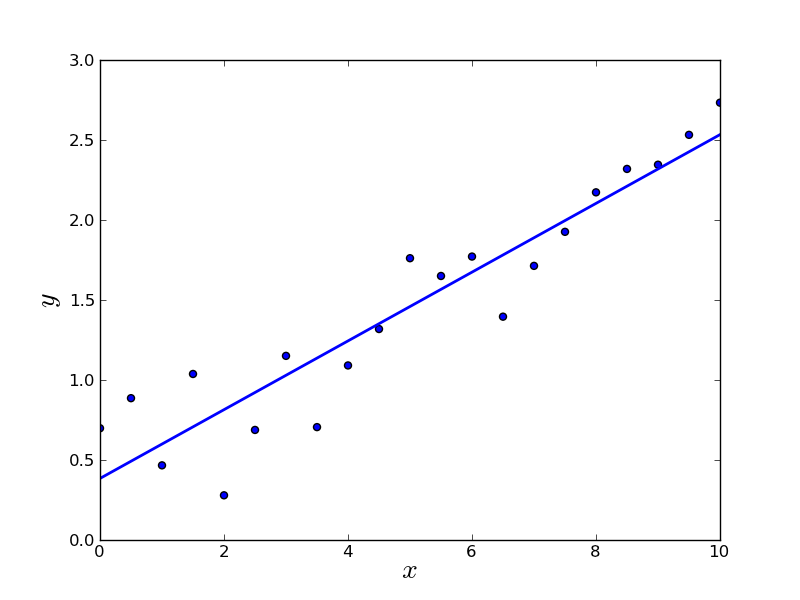
\includegraphics[width = 0.8\textwidth]{LR.png}
\end{center}
\begin{enumerate}
%%%%%%%%%%%%%%%%%%%%%%%%%%%%%%%%%%%%%
\item Fit a line to data points
$$
(x_1,y_1),\quad (x_2,y_2),\quad...,\quad (x_m,y_m)
$$
%%%%%%%%%%%%%%%%%%%%%%%%%%%%%%%%%%%%%
\item Find $y = ax+b$ such that
$$
\begin{bmatrix}
x_1 & 1\\
x_2 & 1\\
\vdots & \vdots\\
x_m & 1
\end{bmatrix}\begin{bmatrix}
a\\b
\end{bmatrix} = \begin{bmatrix}
y_1\\
y_2\\
\vdots \\
y_m
\end{bmatrix}
$$
Overdetermined system!

%%%%%%%%%%%%%%%%%%%%%%%%%%%%%%%%%%%%%
\item How to solve this overdetermined system? Pick $a$, $b$ to minimize error. 
\begin{itemize}
\item Statistics: minimize $\displaystyle \frac{1}{m} \sum_{i=1}^m(ax_i+b-y_i)^2$
\item Linear algebra: minimize $\|A\vec x -\vec b\|^2$
\item Minimize the difference between prediction and target.
\end{itemize}
\end{enumerate}
\end{enumerate}
%%%%%%%%%%%%%%%%%%%%%%%%%%%%%%%%%%%%%
\item Least square approximation process (draw picture to illustrate, summarize process)
\begin{center}
Find $\vec x$ such that $A\vec x = \vec b$ where $m\gg n$
\end{center}
$$
\downarrow
$$
\begin{center}
Not solvable
\end{center}
$$
\downarrow
$$
\begin{center}
Find $\vec x$ to minimize $\|A\vec x -\vec b\|^2$
\end{center}
$$
\downarrow
$$
\begin{center}
Solve $\displaystyle A\vec x = \text{Proj}_{\text{Col } A}\vec b$
\end{center}
$$
\downarrow
$$
\begin{center}
Find $\vec x$ such that $ A\vec x-\vec b$ is orthogonal to Col $A$
\end{center}
$$
\downarrow
$$
\begin{center}
Find $\vec x$ such that $A\vec x-\vec b$ is in (Col $A)^\perp$
\end{center}
%%%%%%%%%%%%%%%%%%%%%%%%%%%%%%%%%%%%%
\item Column space and null space
Let $W$ be a subspace of vector space $V$
\begin{itemize}
\item $W^\perp$: the orthogonal compliment of subspace $W$.
\begin{itemize}
\item $W^\perp$: all vectors in $V$ that are orthogonal to $W$
\item $W^\perp$: all vectors $\vec x$ in $V$ satisfying $
\vec x\cdot\vec w = 0$ for any $\vec w$ in W.
\item $W^\perp$: all vectors $\vec x$ in $V$ satisfying $
\vec x\cdot\vec w = 0$ for any $\vec w$ in a spanning set of W.
\end{itemize}
\item (Col $A)^\perp$: all vectors $\vec x$ in $R^n$ satisfying $
\vec x\cdot\vec a_j = 0$, $1\leq j\leq n$
\item Null $A$: the null space of $A$ (the solution space of $A\vec x = 0$)
\end{itemize}
%%%%%%%%%%%%%%%%%%%%%%%%%%%%%%%%%%%%%
\item A key result on two of the fundamental subspaces of linear algebra.
\begin{thm}
(Col $A)^\perp$ = Null $(A^T)$
\end{thm}
Why is this true? Let $\vec{x} \in $ NULL$(A^T)$. Then $\vec{x} \cdot \vec{a_i}=0$ for all columns of $A$.

%%%%%%%%%%%%%%%%%%%%%%%%%%%%%%%%%%%%%
\item How does this translate to least squares? $A\vec{x}=\vec{b}$ is not solveable. Then, $\vec{b}$ is not in Col$(A)$, but $A\vec{x}$ is. Draw a picture of the column space with $\vec{b}$. So our problems translates.
\begin{center}
Find $\vec x$ $A\vec{x}$ is closest to $\vec{b}$. 
\end{center}
$$
\downarrow
$$
\begin{center}
Find $\vec x$ such that $ A\vec x-\vec b \in ($Col $A)^\perp$ \\ (since the projection is the best approximation)
\end{center}
$$
\downarrow
$$
\begin{center}
Find $\vec x$ such that $ A\vec x-\vec b \in $ Null $(A^T)$
\end{center}
$$
\downarrow
$$
\begin{center}
Find $\vec x$ such that $ A^T(A\vec{x} - \vec{b}) = 0$
\end{center}
$$
\downarrow
$$
\begin{center}
Find $\vec x$ which solves the \emph{normal equations} $ A^TA\vec{x} = A^T \vec{b} \quad \Rightarrow \quad \vec{x} = (A^TA)^{-1}A\vec{b}$
\end{center}
\begin{thm}
The least square approximation of $A\vec x = \vec b$ is the solution of the {\bf normal equation}
$$
A^TA\vec x = A^T \vec b
$$
\end{thm}
Why is it called the normal equations? Now we know. Orthogonality.

%%%%%%%%%%%%%%%%%%%%%%%%%%%%%%%%%%%%%
\item Calculus approach
\begin{center}
Find $\vec x$ to minimize $\|A\vec x-\vec b\|^2$
\end{center}
$$
\downarrow
$$
\begin{center}
$
\displaystyle\frac{d \|A\vec x-\vec b\|^2}{d\vec x} = 0
$
\end{center}
$$
\downarrow
$$
\begin{center}
$
\displaystyle A^TA\vec x = A^T \vec b
$
\end{center}

%%%%%%%%%%%%%%%%%%%%%%%%%%%%%%%%%%%%%
\item QR approach
$A = QR$
\begin{itemize}
\item Col $A$ = Col $Q$
\item $\displaystyle \text{Proj}_{\text{Col }Q} \vec b = QQ^T \vec b$
\end{itemize}
\begin{center}
Solve $A\vec x = \displaystyle \text{Proj}_{\text{Col }A} \vec b$
\end{center}
$$
\downarrow
$$
\begin{center}
Solve $R\vec x = Q^T\vec b$
\end{center}

%%%%%%%%%%%%%%%%%%%%%%%%%%%%%%%%%%%%%
\item Normal equation $A^TA\vec x = A^T \vec b$ summary
\begin{itemize}
\item Projection idea
\item Calculus idea
\item n by n linear system
\item Easy to use
\item Not efficient (less than 1000 by 1000)
\item Numerically unstable.
\end{itemize}

%%%%%%%%%%%%%%%%%%%%%%%%%%%%%%%%%%%%%
\item General least square problem
\begin{itemize}
\item Multi-variable linear regression
$$
y = \theta_0 + \theta_1x_1+\theta_2x_2+\dots+\theta_nx_n  = \vec x^T\vec \theta
$$
\item Polynomial regression
$$
y = \theta_0 + \theta_1x+\theta_2x^2+\dots+\theta_nx^n$$
\item $X\vec \theta = \vec y $
\begin{itemize}
\item Row of $X$: $x$ values of samples
\item Columns of $X$: variables
\item $\vec y $: $y$ value of samples
\item $\vec \theta$: parameter of the model
\end{itemize}
\item Find $\theta$ to minimize 
$$
\|X\vec \theta- y\|^2, \quad \text{or equivalently}\quad \frac{1}{m}((\vec x_i)^T\vec \theta-y_i)^2
$$
\end{itemize}

%%%%%%%%%%%%%%%%%%%%%%%%%%%%%%%%%%%%%
\item Gradient descent method: Define $\displaystyle J(\vec \theta) = \frac{1}{m}\sum_{i=1}^m(\theta_0+ \theta_1x^{(i)}_1+\dots+ \theta_nx^{(i)}_n -y_i)^2$\\[0.2in]

{\bf Gradient descent method} to minimize $J(\vec \theta)$
$$
\vec \theta : = \vec\theta - \frac{dJ(\vec \theta)}{d\vec\theta}
$$
Entrywise ($i$ is variable index, $n$ is number of iteration)
\begin{equation*}
\begin{split}
\theta_{j} &: = \theta_j - \frac{\partial(J(\vec\theta))}{\partial \theta_j}\\
& = \theta_j - (\theta_0+ \theta_1x^{(i)}_1+\dots+ \theta_nx^{(i)}_n -y_i)\cdot x^{(i)}_j
\end{split}
\end{equation*}

%%%%%%%%%%%%%%%%%%%%%%%%%%%%%%%%%%%%%
\item Optimization problem: The least \st{square} problem
\begin{center}
Find $\theta$ to minimize $J(\theta)$
\end{center}
\begin{itemize}
\item Minimize/Maximize
\item Gradient descent
\begin{itemize}
\item Fast
\item Numerical partial derivatives
\end{itemize}
\item Restriction
\item Optimizations
\end{itemize}

%%%%%%%%%%%%%%%%%%%%%%%%%%%%%%%%%%%%%
\item Optimizations
\begin{itemize}
\item $J(\theta)$ = prediction error: regression
\item $J(\theta)$ = cost function: machine learning
\item $J(\theta)$ = profit: business strategy
\item  $J(\theta)$ = traveling time: route/schedule making
\item $J(\theta)$ = space occupancy: warehouse efficiencey
\end{itemize}


%%%%%%%%%%%%%%%%%%%%%%%%%%%%%%%%%%%%%
\item Example:
\begin{itemize}
\item Class scheduling
\item John Deere intern
\end{itemize}
\end{enumerate}



%%%%%%%%%%%%%%%%%%%%%%%%%%%%%%%%%%%%%
%%%%%%%%%%%%%%%%%%%%%%%%%%%%%%%%%%%%%
\section{Chapter 4: Numerical Interpolation}
%%%%%%%%%%%%%%%%%%%%%%%%%%%%%%%%%%%%%
%%%%%%%%%%%%%%%%%%%%%%%%%%%%%%%%%%%%%

%%%%%%%%%%%%%%%%%%%%%%%%%%%%%%%%%%%%%
%%%%%%%%%%%%%%%%%%%%%%%%%%%%%%%%%%%%%
\subsection{4.1 Polynomial interpolation}
%%%%%%%%%%%%%%%%%%%%%%%%%%%%%%%%%%%%%
%%%%%%%%%%%%%%%%%%%%%%%%%%%%%%%%%%%%%

\begin{enumerate}
%%%%%%%%%%%%%%%%%%%%%%%%%%%%%%%%%%%%%
\item Idea: 
\begin{enumerate}
%%%%%%%%%%%%%%%%%%%%%%%%%%%%%%%%%%%%%
\item Math problem
\begin{center}
Given a graph $\rightarrow$ Produce a formula $f(x)$
\end{center}
%%%%%%%%%%%%%%%%%%%%%%%%%%%%%%%%%%%%%
\item Numerical problem
\begin{center}
Sample points from the real world  $\rightarrow$ Formula $f(x)$ (usually a polynomial)
\end{center}
\end{enumerate}


%%%%%%%%%%%%%%%%%%%%%%%%%%%%%%%%%%%%%
\item Construction: Notation
\begin{itemize}
\item Sample point: $(x_i,y_i)$, $0\leq i\leq n$. Total of $(n+1)$ points here.
\item Polynomial: $p(x)$
\end{itemize}
\begin{thm}
For distinct points $x_0$, $x_1$,..., $x_n$, and $y_0$, $y_1$,..., $y_n$, there's a unique polynomial p of degree ${\color{red} \leq} n$ such that 
$$
p(x_i) = y_i,\quad 0\leq i\leq n.
$$
\end{thm}

%%%%%%%%%%%%%%%%%%%%%%%%%%%%%%%%%%%%%
\item Finding the interpolating polynomial
\begin{enumerate}
%%%%%%%%%%%%%%%%%%%%%%%%%%%%%%%%%%%%%
\item Given distinct points $x_0$, $x_1$,..., $x_n$, and $y_0$, $y_1$,..., $y_n$, find the polynomial $p$ of degree $\leq n$ such that 
$$
p(x_i) = y_i,\quad 0\leq i\leq n.
$$
Let
$$
p(x) = a_0 + a_1x + a_2x + \dots + a_nx^n
$$
Find the coefficients $a_i$, $0\leq i\leq n$.
%%%%%%%%%%%%%%%%%%%%%%%%%%%%%%%%%%%%%
\item Why is polynomial a good choice? Simplest idea. Also, it works....
\begin{thm}
(Weierstrauss Approximation Theorem)
Let $f$ be continuous on $[a,b]$. Then for any $\epsilon >0 $, there exists a polynomial $p(x)$ such that 
\[
|f(x) - p(x)| < \epsilon \quad \text{on [a,b]}
\]
\end{thm}
Note, we don't know the degree of said polynomial or how to find it.
%%%%%%%%%%%%%%%%%%%%%%%%%%%%%%%%%%%%%
\item Example: find a degree two polynomial passing through points
$$
(0,1), \quad (1,3),\quad (-1,1)
$$
We will highlight 3 main ways for tackling this problem.
\end{enumerate}


%%%%%%%%%%%%%%%%%%%%%%%%%%%%%%%%%%%%%
\item {\bf Method 1:} Linear algebra and the Vandermonde matrix.
\begin{enumerate}
\item Solve $V\vec x = \vec b$
$$
\begin{bmatrix}
1 & x_0 & x_0^2 & x_0^3 & \dots& x_0^n\\
1 & x_1 & x_1^2 & x_1^3 &\dots & x_1^n\\
 \vdots&\vdots&\vdots&\vdots &&\vdots\\
1 & x_n & x_n^2 & x_n^3 &\dots & x_n^n
\end{bmatrix}_V
\begin{bmatrix}
a_0\\
a_1\\
\vdots\\
a_n
\end{bmatrix}_{\vec x} = \begin{bmatrix}
y_0\\
y_1\\
\vdots\\
y_n
\end{bmatrix}_{\vec b}
$$
$V$: Vandermonde matrix 

%%%%%%%%%%%%%%%%%%%%%%%%%%%%%%%%%%%%%
\item Example: find a degree two polynomial passing through points
$$
(0,1), \quad (1,3),\quad (-1,1)
$$


%%%%%%%%%%%%%%%%%%%%%%%%%%%%%%%%%%%%%
\item The invertibility of Vandermonde matrix
\begin{enumerate}
%%%%%%%%%%%%%%%%%%%%%%%%%%%%%%%%%%%%%
\item Is the linear system $V\vec x = \vec b$ consistent?
\begin{itemize}
\item $V$: $n+1 \times n+1$
\item Is $V$ invertible?
\end{itemize}
\begin{thm}[The invertibility of Vandermonde matrix]
%%%%%%%%%%%%%%%%%%%%%%%%%%%%%%%%%%%%%
\item The determinant 
\begin{center}
$
\displaystyle\det (V) = \prod_{1\leq i\neq j\leq n} (x_i-x_j)
$
\end{center}
\end{thm}
\begin{itemize}
\item $V$ is invertible if $x_0$, $x_1$,\dots, $x_n$ are distinct points.
\end{itemize}
\end{enumerate}

%%%%%%%%%%%%%%%%%%%%%%%%%%%%%%%%%%%%%
\item Vandemonde matrix is a BAD method
\begin{itemize}
\item We usually take lots of sample points to increase the accuracy.
\item Solving large linear system is expensive.
\item $\det V$ is usually very small ($V$ is ill-conditioned).
\item High power result in extremely huge/small matrix entries
\end{itemize}
\end{enumerate}


%%%%%%%%%%%%%%%%%%%%%%%%%%%%%%%%%%%%%
\item {\bf Method 2:} Newton interpolating polynomial
\begin{enumerate}
\item Idea (Newton form): Find $a_0$, $a_1$,\dots,$a_n$ in
\begin{equation}\nonumber
\begin{split}
p(x) = &a_0 + a_1(x-x_0) + a_2[(x-x_0)(x-x_1)] + ... \\
& + a_n[(x-x_0)(x-x_1)\dots(x-x_{n-1})]
\end{split}
\end{equation}
such that
$$
p(x_i) = y_i,\quad 0\leq i\leq n.
$$
Can you see why this works? Why is it constructed this way?

%%%%%%%%%%%%%%%%%%%%%%%%%%%%%%%%%%%%%
\item Example: find a degree two polynomial passing through points
$$
(0,1), \quad (1,3),\quad (-1,1)
$$
Let
$$
p(x) = a_0 + a_1x + a_2 x(x-1)
$$
Plug in 
\begin{align*}
(0,1):\quad a_0 = 1\\
(1,3): \quad a_1 = 2\\
(-1,1): \quad a_2 = 1
\end{align*}
Thus
$$
p(x) = 1 + 2x+x(x-1) = x^2+x+1
$$

%%%%%%%%%%%%%%%%%%%%%%%%%%%%%%%%%%%%%
\item Algorithm
\begin{equation}
\nonumber
\begin{split}
& a_0 = y_0\\
& a_1 = \frac{y_1-a_0}{x_1-x_0}\\
& a_2 = \frac{y_2-a_0-a_1(x_2-x_0)}{(x_2-x_0)(x_2-x_1)}\\
& a_3 = \frac{y_3-a_0-a_1(x_3-x_0)-a_2(x_3-x_0)(x_3-x_1)}{(x_3-x_0)(x_3-x_1)(x_3-x_2)}\\
& \cdots
\end{split}
\end{equation}
There appears to be recursion going on. Compactify this schiznit. 
%%%%%%%%%%%%%%%%%%%%%%%%%%%%%%%%%%%%%
\item Let $a_n: = f[x_0,x_1,x_2,..., x_n]$, then
\begin{thm}[Newton's divided difference formula]
$$f[x_0,x_1,...,x_k] = \frac{f[x_1,...,x_k]-f[x_0,...,x_{k-1}]}{x_k-x_0}$$
\end{thm}
\begin{itemize}
\item $f[x_0,x_1, ..., x_n]:$ Newton's $n^{th}$ divided difference
\item The order of the sample points doesn't matter
\item Level $n\rightarrow n+1$
\item Connection with linear function.
\end{itemize}

%%%%%%%%%%%%%%%%%%%%%%%%%%%%%%%%%%%%%
\item Divided differences matrix 
$$
\begin{bmatrix}
D_{11} & 0 & \dots & \dots & 0 \\
D_{21} & D_{22} & \dots & \dots & 0 \\
\vdots & \vdots && & \vdots \\
D_{n1} & D_{n2} & \dots & \dots & D_{nn}
\end{bmatrix}
$$
\begin{itemize}
\item $D$ is $n+1$ by $n+1$.
\item $D$ is lower triangular.
\item $a_i = D(i+1,i+1)$, for $0\leq i\leq n$.
\end{itemize}

%%%%%%%%%%%%%%%%%%%%%%%%%%%%%%%%%%%%%
\item Algorithm: Construct $D$ (x, y are the columns vectors of the data points)
\begin{verbatim}
D(:,1) = y;
for j = 2 : n
    for i = j : n
    	   D(i,j)=(D(i,j-1)-D(i-1,j-1))/(x(i)-x(i-j+1));
    end
end
\end{verbatim}

%%%%%%%%%%%%%%%%%%%%%%%%%%%%%%%%%%%%%
\item Rewrite above example in this format. 
\end{enumerate}


%%%%%%%%%%%%%%%%%%%%%%%%%%%%%%%%%%%%%
\item {\bf Method 3} Lagrange polynomial
\begin{enumerate}
\item Idea of Lagrange (Cardinal functions): Given $x_0$, $x_1$, \dots, $x_n$, the cardinal functions $l_0$, $l_1$, \dots, $l_n$ are degree $n$ polynomials satisfying
$$
l_i(x_j) = \delta_{ij} := \left\{
\begin{array}{ll}
0, & i\neq j,\\
1, & i = j.
\end{array}
\right.
$$ 
Thus the interpolating polynomial
$$
p(x) = \sum_{i=0}^n l_i(x)y_i
$$
Thus,
$$
l_i(x) = \prod_{j=0, ~ j\neq i}^n \frac{x-x_j}{x_i-x_j}
$$

%%%%%%%%%%%%%%%%%%%%%%%%%%%%%%%%%%%%%
\item Example: use Lagrange interpolating polynomial to  find a degree two polynomial passing through points
$$
(0,1), \quad (1,3),\quad (-1,1)
$$
Find
\begin{equation}
\nonumber
\begin{split}
& l_0(x) = \frac{(x-1)(x+1)}{(0-1)(0+1)} = 1-x^2\\
& l_1(x) = \frac{x(x+1)}{(1-0)(1+1)} = \frac{x(x+1)}{2}\\
& l_2(x) = \frac{x(x-1)}{(-1-0)(-1-1)} = \frac{x(x-1)}{2}
\end{split}
\end{equation}
Then
$$
p(x) = \sum_{i=0}^2 l_i(x)y_i = l_0(x) + 3l_1(x)+l_2 (x) = x^2+x+1
$$
\end{enumerate}
\end{enumerate}


%%%%%%%%%%%%%%%%%%%%%%%%%%%%%%%%%%%%%
%%%%%%%%%%%%%%%%%%%%%%%%%%%%%%%%%%%%%
\subsection{4.2 Numerical analysis of polynomial interpolation}
%%%%%%%%%%%%%%%%%%%%%%%%%%%%%%%%%%%%%
%%%%%%%%%%%%%%%%%%%%%%%%%%%%%%%%%%%%%

\begin{enumerate}
%%%%%%%%%%%%%%%%%%%%%%%%%%%%%%%%%%%%%
\item Comparison:
\begin{enumerate} 
%%%%%%%%%%%%%%%%%%%%%%%%%%%%%%%%%%%%%
\item Vandermonde matrix method (we should avoid this method)
\begin{itemize}
\item Nice structure
\item Expensive to compute
\item The matrix is usually ill-conditioned 
\end{itemize}
%%%%%%%%%%%%%%%%%%%%%%%%%%%%%%%%%%%%%
\item Newton interpolating method (most practical)
\begin{itemize}
\item Easy to code
\item The most efficient
\end{itemize}
%%%%%%%%%%%%%%%%%%%%%%%%%%%%%%%%%%%%%
\item Lagrange interpolating method
\begin{itemize}
\item Easy to write down (theoretical uses)
\item Not so efficient $(\mathcal{O}(n^2))$
\end{itemize}
\end{enumerate}


%%%%%%%%%%%%%%%%%%%%%%%%%%%%%%%%%%%%%
\item Error estimate
\begin{enumerate}
%%%%%%%%%%%%%%%%%%%%%%%%%%%%%%%%%%%%%
\item 
\begin{thm}[Error estimate for polynomial interpolation]
Let $p$ be the interpolating polynomial of $f(x)$ at $x_0$, \dots, $x_n$, which belongs to an interval $[a,b]$. If $f^{(n+1)}(x)$ is continuous, then there is a $\xi$ in $(a,b)$ for which
$$
f(x)-p(x) = \frac{1}{(n+1)!}f^{(n+1)}(\xi)\prod_{i=0}^n(x-x_i),\quad a\leq x\leq b.
$$
\\[0.1in]
\end{thm}
%%%%%%%%%%%%%%%%%%%%%%%%%%%%%%%%%%%%%
\item Proof: \\
For $x=x_i$, this works. Assume $x\neq x_i$ and denote
\[
w(x) = (x-x_0)(x-x_1)\cdots (x-x_n)
\]
Consider $x$ as fixed and define
\[
c = \frac{f(x)-p(x)}{w(x)}.
\]
Then, define $g(t)$ in variable $t$ as
\[
g(t) = f(t)-p(t)-cw(t).
\]
Then, $g$ is $(n+1)$ times differentiable since $f$ is and $p,w$ are polynomials. Also,
\[
g(x_i)=0, \quad g(x)=0
\]
So $g$ has $(n+2)$ zeros on $[a,b]$. Repeating Rolle's theorem, 
\[
g' \quad \text{has $(n+1)$ zeros}
\]
\[
g'' \quad \text{has $n$ zeros}
\]
\[
\vdots
\]
\[
g^{n+1} \quad \text{has $1$ zero on $[a,b]$}
\]
Then,
\[
g^{(n+1)}(\xi) = f^{(n+1)}(\xi) - p^{(n+1)}(\xi) - cw^{(n+1)}(\xi) = f^{(n+1)}(\xi) - 0 - c(n+1)! = 0
\]
\[
\Rightarrow \frac{f(x)-p(x)}{w(x)} = \frac{f^{(n+1)}(\xi)}{(n+1)!}
\]
Rearranging, we are done.
\[
f(x) - p(x) = \frac{f^{(n+1)}(\xi)}{(n+1)!}\prod_{i=0}^n (x-x_i)
\]

%%%%%%%%%%%%%%%%%%%%%%%%%%%%%%%%%%%%%
\item \begin{thm}[Rolle's theorem]
If $f(x)$ is continuously differentiable on $(a,b)$ and $f(a) = f(b) = 0$, then there's a $\xi$ in $(a,b)$ such that 
$$
f'(\xi) = 0
$$
\end{thm}
\end{enumerate}

%%%%%%%%%%%%%%%%%%%%%%%%%%%%%%%%%%%%%
\item The convergence analysis
\begin{itemize}
\item Require $f^{(i)}(x)$ is continuous for $0\leq i\leq n+1$
\item More sample points $\rightarrow$ better accuracy?
$$
f(x) - p(x) = \frac{f^{(n+1)}(\xi)}{(n+1)!}\prod_{i=0}^n (x-x_i)
$$
\item In general, higher order (more sample points) {\color{red} does not} guaranteed better accuracy!!
$$
f^{(n+1)}(\xi)\quad  \text{can grow fast as $n$ increases}
$$
\end{itemize}

%%%%%%%%%%%%%%%%%%%%%%%%%%%%%%%%%%%%%
\item Runge function: 
$$
f(x)  = \frac{1}{1+25x^2}
$$
\begin{itemize}
\item $f(x)$ is infinitely many differentiable on $(-1,1)$
\item Find the interpolating polynomial on $[-1,1]$
\item Use sample points with equal distance
\end{itemize}
The error blow up because
$$
f^{(n+1)}(\xi)\quad  \text{grow very fast as $n$ increases}
$$

%%%%%%%%%%%%%%%%%%%%%%%%%%%%%%%%%%%%%
\item Cure for the high error:
\begin{itemize}
\item Choose sample points carefully: \href{https://en.wikipedia.org/wiki/Chebyshev_nodes}{{\color{red}Chebyshev nodes}}
\item Remove the requirement 
$$
p(x_i) = y_i
$$
Regression (least square)
\item Use many low degree interpolation instead of one high degree.
\end{itemize}

%%%%%%%%%%%%%%%%%%%%%%%%%%%%%%%%%%%%%
\item Comparison with interpolation and regression
\begin{itemize}
\item High order regression
\item Interpolation is an ``overfitting" regression
\item Train error vs prediction error
\begin{itemize}
\item Training: sample points
\item Prediction: evaluation points
\end{itemize}
\item Memorizing too much won't let you learn.
\end{itemize}

%%%%%%%%%%%%%%%%%%%%%%%%%%%%%%%%%%%%%
\item Evaluating polynomial interpolation
\begin{itemize}
\item Test function $f(x)$
\begin{itemize}
\item Standard ones
\item Good ones
\item Bad ones
\end{itemize}
\item Evaluation points $(x_i,f(x_i))$: different from the sample points
\item Homework
\end{itemize}

%%%%%%%%%%%%%%%%%%%%%%%%%%%%%%%%%%%%%
\item Idea behind the interpolation polynomial \\
Vector space $V:=$ all infinitely continuous differentiable functions
\begin{itemize}
\item dim $V = \infty$ 
\item A basis of $V$:
$$
1,\quad x, \quad  x^2, \quad x^3, \quad ...\quad x^n\quad ...
$$
\item Then any $f(x)$ in $V$ can be written as a linear combination 
$$
f(x) = a_0+a_1x+a_2x^2+\cdots + a_nx^n
$$
\item Not doable.
\end{itemize}


%%%%%%%%%%%%%%%%%%%%%%%%%%%%%%%%%%%%%
\item Idea behind interpolation polynomial
\begin{itemize}
\item Subspace $H$ = span $\{1,x,x^2,...,x_n\}$
\item Projection of $f$
$$
\bar f = Proj_{H}f
$$
\item Find the linear combination 
$$
\bar f = a_0 + a_1x+ a_2x^2+ \cdots + a_nx^n
$$
\item Error $f-\bar f$ is determined by the subspace $H$.
\end{itemize}

%%%%%%%%%%%%%%%%%%%%%%%%%%%%%%%%%%%%%
\item Wrap up \\
Infinitely dimensional $V$  -- Basis B: infinitely many vectors
\begin{center}
Find the linear combination of $f$ in $V$ using the basis
\end{center}
Subspace $H$  -- Basis: a subset of $B$
\begin{center}
Find the linear combination of $\bar f$ in $H$ using the basis
\end{center}
where $\bar f$ is the projection of $f$ on $H$.

%%%%%%%%%%%%%%%%%%%%%%%%%%%%%%%%%%%%%
\item Fourier transform: \\
Signal space $V$: all period functions (formally)
\begin{itemize}
\item Basis
$$
1,\quad \sin(x),\quad \cos(x),\quad \sin(2x),\quad \cos(2x),\quad\dots
$$
\item Find the linear combination of $f$ in $V$ such that
$$
f = C + a_1\sin(x) + b_1\cos(x)+a_2\sin(2x)+b_2\cos(2x)+\cdots
$$
\end{itemize}
\begin{center} 
The Fourier Series
\url{https://en.wikipedia.org/wiki/Doppler_spectroscopy} \\
\url{https://www.kaggle.com/mrisdal/open-exoplanet-catalogue}
\end{center}

\end{enumerate}


%%%%%%%%%%%%%%%%%%%%%%%%%%%%%%%%%%%%%
%%%%%%%%%%%%%%%%%%%%%%%%%%%%%%%%%%%%%
\subsection{4.3 Splines}
%%%%%%%%%%%%%%%%%%%%%%%%%%%%%%%%%%%%%
%%%%%%%%%%%%%%%%%%%%%%%%%%%%%%%%%%%%%

\begin{enumerate}
%%%%%%%%%%%%%%%%%%%%%%%%%%%%%%%%%%%%%
\item Goal: Reduce the interpolating error. How?
\begin{enumerate}
\item \st{More sample points (higher order)} (issue is with equally spaced nodes)
\item Choose sample points carefully (Chebyshev)
\item The spline function: piecewise low degree interpolation
\end{enumerate}
Matlab example to illustrate these three.

%%%%%%%%%%%%%%%%%%%%%%%%%%%%%%%%%%%%%
\item Linear spline function: The linear spline function of $f(x)$ on $[a,b]$
\begin{enumerate}
\item Draw picture to illustrate.
\item Knots: sample points on interval $[a,b]$
$$
x_0, x_1,\dots,x_n,\quad\text{where}\quad  x_0 = a,\quad x_n = b
$$
\item Partition of [a,b]: $[x_{i-1}, x_i]$, \quad $1\leq i \leq n$
\item In each interval, define a linear function $p_i(x)$ such that
$$
p_i(x_{i-1}) = f(x_{i-1}),\quad p_i(x_{i}) = f(x_{i}),\quad 1\leq i\leq n
$$
\item Linear piece: for $1\leq i\leq n$
$$
p_i(x) = f(x_{i-1})\frac{x-x_{i}}{x_{i-1}-x_{i}} +  f(x_{i})\frac{x-x_{i-1}}{x_{i}-x_{i-1}}
$$
\item Linear spline function
$$
p(x) = p_i(x),\quad \text{for}\quad x\in [x_{i-1},x_{i}), \quad 1\leq i \leq n
$$
\item If we have a \emph{uniform mesh}, rewrite with $h = \Delta x = x_i - x_{i=1}$.
\end{enumerate}

%%%%%%%%%%%%%%%%%%%%%%%%%%%%%%%%%%%%%
\item Advantages/disadvantages of Linear spline function
\begin{center}
One high order $p(x)$ \quad {\bf VS} \quad multiple lower order $p_i(x)$
\end{center}
\begin{itemize}
\item Adv: More sample points $\rightarrow$ better accuracy
\item Adv: Efficient computation
\item Adv: Works for weird shape (non-functionss)
\item Dis: Sacrifice smoothness
\begin{itemize}
\item Ultimate solution: Higher order spline functions (cubic is king)
\end{itemize}
\end{itemize}

%%%%%%%%%%%%%%%%%%%%%%%%%%%%%%%%%%%%%
\item Spline function definition: A function $S(x)$ is called a spline of degree $k$ on $[a,b]$ if 
\begin{itemize}
\item Domain of $S$: $[a,b]$
\item Knots: $a = x_0 < x_1,\dots < x_n = b$
\item $S$ is a polynomial of degree less or equal to $k$ on each subinterval $[x_i,x_{i-1}]$.
\item $S'$, $S''$,\dots, $S^{(k-1)}$ is continuous
\end{itemize}
Linear spline function is the degree 1 spline function.


%%%%%%%%%%%%%%%%%%%%%%%%%%%%%%%%%%%%%
\item Degree 2 spline function
\begin{enumerate}
\item Continuity
$$
S_i(x_{i-1}) = f(x_{i-1}),\quad S_i(x_{i}) = f(x_{i}),\quad {\color{red} 1\leq i \leq n}
$$
\item Continuity of $S'(x)$ on interior nodes only.
$$
S_i'(x_{i}) = S_{i+1}'(x_{i}), \quad {\color{red}  1\leq i \leq n-1}
$$

\end{enumerate}

\begin{itemize}
\item No. of variables: $3n$
\item No. of equations: $n + n + n-1 = 3n-1$
\item Manually add: $S'(x_0) = f'(x_0)$
\end{itemize}



%%%%%%%%%%%%%%%%%%%%%%%%%%%%%%%%%%%%%
\item Cubic spline function: Degree 3 spline function satisfies
$$
S_i(x_{i-1}) = f(x_{i-1}),\quad S_i(x_{i}) = f(x_{i}),\quad 1\leq i \leq n
$$
$$
S_i'(x_{i}) = S_{i+1}'(x_{i}), \quad S_i''(x_{i}) = S_{i+1}''(x_{i}), \quad 1\leq i \leq n-1
$$
\begin{itemize}
\item No. of variables: $4n$
\item No. of equations: $4n-2$ (Nice added flexibility here.)
\item Manually add 2 equations: Many choices here. What is the interpretation of these conditions?
\begin{itemize}
\item {\color{red} Natural} cubic spline:
$$
S_1''(x_0) = S_n''(x_n) = 0
$$
\item {\color{red} Complete} cubic spline:
$$
S_1'(x_0) = f'(x_0),\quad S_n'(x_n) = f'(x_n)
$$
\end{itemize}
\item First derivative: increasing/decreasing
\item Second derivative: concavity/curvature
\end{itemize}


%%%%%%%%%%%%%%%%%%%%%%%%%%%%%%%%%%%%%
\item Example: Find the natural cubic spline function through knots
$$
(-1,1),\quad (0,2), \quad (1,-1)
$$
\begin{enumerate}
%%%%%%%%%%%%%%%%%%%%%%%%%%%%%%%%%%%%%
\item Define
\begin{eqnarray*}
S_1(x) = a_1x^3+ b_1x^2 + c_1x + d_1\\
S_2(x) = a_2x^3+ b_2x^2 + c_2x + d_2
\end{eqnarray*}
%%%%%%%%%%%%%%%%%%%%%%%%%%%%%%%%%%%%%
\item Need 8 equations!
$$
\left\{
\begin{array}{llll}
S_1(-1) = 1, &  
S_1(0) = 2, & 
S_2(0) = 2, & 
S_2(1) = -1,\\
S'_1(0) = S'_2(0), & 
S''_1(0) = S''_2(0), &
S_1''(-1) = 0, & 
S_2''(1) = 0
\end{array}
\right.,\quad$$
that is 
$$
\left\{
\begin{array}{l}
 a_1(-1)^3+ b_1(-1)^2 + c_1(-1) + d_1 = 1\\
a_1(0)^3+ b_1(0)^2 + c_1(0) + d_1  = 2\\
a_2(0)^3+ b_2(0)^2 + c_2(0) + d_2 = 2\\
a_2(1)^3+ b_2(1)^2 + c_2(1) + d_2 = -1\\
3a_1(0)^2 + 2b_1(0) + c_1 = 3a_2(0)^2 + 2b_2(0) + c_2\\
6a_1(0)+ 2b_1 = 6a_2(0)+ 2b_2\\
6a_1(-1) + 2b_1  = 0\\
6a_2(1) + 2b_2 = 0
\end{array}
\right.
$$
%%%%%%%%%%%%%%%%%%%%%%%%%%%%%%%%%%%%%
\item Solution
\begin{eqnarray*}
a_1 = -1,\quad b_1 = -3, \quad c_1 = -1, \quad d_1 = 2\\
a_2 = 1, \quad b_2 = -3, \quad c_2 = -1, \quad d_2 = 2
\end{eqnarray*}
thus the natural spline function
\begin{eqnarray*}
S(x) = -x^3-3x^2-x+2,\quad -1\leq x\leq 0\\
S(x) = x^3-3x^2-x+2,\quad 0\leq x\leq 1
\end{eqnarray*}
We definitely need a better algorithm!
\end{enumerate}


%%%%%%%%%%%%%%%%%%%%%%%%%%%%%%%%%%%%%
\item Algorithm: For finding any cubic spline.
\begin{enumerate}
%%%%%%%%%%%%%%%%%%%%%%%%%%%%%%%%%%%%%
\item Goal: For a given function $f$ and $(n+1)$ nodes $x_i$,	
$$
S_i(x_{i-1}) = f(x_{i-1}),\quad S_i(x_{i}) = f(x_{i}),\quad 1\leq i \leq n
$$
$$
S_i'(x_{i}) = S_{i+1}'(x_{i}), \quad S_i''(x_{i}) = S_{i+1}''(x_{i}), \quad 1\leq i \leq n-1
$$
Check off these conditions as we go.
%%%%%%%%%%%%%%%%%%%%%%%%%%%%%%%%%%%%%
\item Assign 
$$
z_i = S''(x_i),\quad 1\leq i\leq n-1
$$ Since $S(x)$ is cubic, $S''(x)$ is linear. Therefore
$$
S''_i(x) = z_{i-1}\frac{x-x_{i}}{x_{i-1}-x_{i}} + z_{i}\frac{x-x_{i-1}}{x_{i}-x_{i-1}}, \quad x_{i-1}\leq x\leq x_{i}
$$
Assume uniform partition with step $h$
\begin{itemize}
\item $x_{i}-x_{i-1} = h$ for $1\leq i \leq n$
\item $x_i = x_0 + ih$ for $1\leq i \leq n$
\end{itemize}
%%%%%%%%%%%%%%%%%%%%%%%%%%%%%%%%%%%%%
\item Then on interval $[x_{i-1},x_{i}]$
$$
 S''_i(x) = z_{i-1}\frac{x_{i}-x}{h} + z_{i}\frac{x-x_{i-1}}{h},
$$
thus
$$
 S'_i(x) = -\frac{1}{h}z_{i-1}\frac{(x_{i}-x)^2}{2} +\frac{1}{h} z_{i}\frac{(x-x_{i-1})^2}{2} + C_i,
$$
Finally for some constant $C_i$, $D_i$
$$
 S_i(x) = \frac{1}{h}z_{i-1}\frac{(x_{i}-x)^3}{6} +\frac{1}{h} z_{i}\frac{(x-x_{i-1})^3}{6} + C_i(x-x_{i-1}) + D_i
$$
Noticed we borrowed some Newton divided difference cleverness here.
%%%%%%%%%%%%%%%%%%%%%%%%%%%%%%%%%%%%%
\item Find $z_i$'s, $C_i$ and $D_i$ in 
$$
 S_i(x) = \frac{1}{h}z_{i-1}
 \frac{(x_{i}-x)^3}{6} +\frac{1}{h} z_{i}\frac{(x-x_{i-1})^3}{6} + C_i(x-x_{i-1}) + D_i
$$
\begin{itemize}
\item Condition (rewrite $f(x_i)$ as $y_i$)
$$
S_i(x_{i-1}) = f(x_{i-1}) \Rightarrow {\color{red} D_i  = y_{i-1} - \frac{h^2}{6}z_{i-1}}
$$
\item Condition
$$
S_i(x_i) = f(x_{i}) \Rightarrow  {\color{red} C_i = \frac{1}{h}\Big[y_i-y_{i-1}+\frac{h^2}{6}(z_{i-1}-z_{i}))\Big]}
$$
\end{itemize}
%%%%%%%%%%%%%%%%%%%%%%%%%%%%%%%%%%%%%
\item Plug $C_i$ and $D_i$ in 
\begin{equation}\nonumber
\begin{split}
 S_i(x) = &\frac{1}{h}z_{i-1}\frac{(x_{i}-x)^3}{6} +\frac{1}{h} z_{i}\frac{(x-x_{i-1})^3}{6} \\
 & + {\color{red} \frac{1}{h}\Big[y_i-y_{i-1}+\frac{h^2}{6}(z_{i-1}-z_{i}))\Big]}(x-x_{i-1}) \\
 & +  {\color{red} y_{i-1}- \frac{h^2}{6}z_{i-1}}
 \end{split}
\end{equation}
%%%%%%%%%%%%%%%%%%%%%%%%%%%%%%%%%%%%%
\item It remains to find $z_i$ for $1\leq i\leq n-1$. Recall:
$$
S'_i(x) = -\frac{1}{h}z_{i-1}\frac{(x_{i}-x)^2}{2} +\frac{1}{h} z_{i}\frac{(x-x_{i-1})^2}{2} + C_i,
$$
For $0\leq i \leq n-1$, condition
$$
S_i'(x_{i}) = S_{i+1}'(x_{i}) \Rightarrow {\color{red} \frac{h}{2}z_i+C_i = -\frac{h}{2}z_{i}+C_{i+1}}
$$
Plug in $C_i$, $C_{i+1}$
\begin{equation*}\nonumber
\begin{split}
\frac{h}{2}z_i&+\frac{1}{h}\Big[y_i-y_{i-1}+\frac{h^2}{6}(z_{i-1}-z_{i}))\Big]\\
 &= -\frac{h}{2}z_{i}+\frac{1}{h}\Big[y_{i+1}-y_{i}+\frac{h^2}{6}(z_{i}-z_{i+1}))\Big]
\end{split}
\end{equation*}
%%%%%%%%%%%%%%%%%%%%%%%%%%%%%%%%%%%%%
\item Finding $z_i$: Organize the terms
$$
\frac{h}{6}z_{i-1} + \frac{2h}{3}z_{i} + \frac{h}{6}z_{i+1} = \frac{1}{h}y_{i-1} -\frac{2}{h}y_i+\frac{1}{h}y_{i+1},\quad 1\leq i\leq n-1
$$
Notice that
$$
z_0 = z_n = 0
$$
Therefore we can rewrite the equations into a linear system
%%%%%%%%%%%%%%%%%%%%%%%%%%%%%%%%%%%%%
\item Solve $[z_1,z_2,\dots,z_{n-1}]^T$ from
$$
\begin{bmatrix}
2h/3 & h/6 & 0 & \dots & \dots & 0\\
h/6 & 2h/3 & h/6 & 0&  \dots & 0\\
\vdots & \vdots & \vdots & \vdots & \vdots & \vdots \\
 0 & \dots  & 0 & h/6 & 2h/3 &h/6\\
 0 & \dots & \dots & 0 & h/6 & 2h/3
\end{bmatrix}
\begin{bmatrix}
z_1\\
z_2\\
\vdots\\
z_{n-2}\\
z_{n-1}
\end{bmatrix} = \begin{bmatrix}
b_1\\
b_2\\
\vdots\\
b_{n-2}\\
b_{n-1}
\end{bmatrix}
$$
where 
$$
b_i = \frac{1}{h}\Big(y_{i-1}-2y_i+y_{i+1}\Big),\quad 1\leq i\leq n-1
$$
\begin{itemize}
\item The coefficient matrix is $n-1$ by $n-1$ and invertible
\item The coefficient matrix is a tri-diagonal matrix
\item For non-uniform partition, use $h_i$ instead of $h$
\end{itemize}
\end{enumerate}

%%%%%%%%%%%%%%%%%%%%%%%%%%%%%%%%%%%%%
\item General curve fitting
\begin{itemize}
\item Non-function
\item Data fitting
\item 3-D curve fitting
\item 3-D spline plane
\end{itemize}

%%%%%%%%%%%%%%%%%%%%%%%%%%%%%%%%%%%%%
\item Spline function: Advantage 
\begin{itemize}
\item Low order polynomial
\item More sample points implies better accuracy
\item Non-function
\item Data interpolation
\item Works for 3-D
\item Surface fitting
\end{itemize}

%%%%%%%%%%%%%%%%%%%%%%%%%%%%%%%%%%%%%
\item Error analysis: Error estimate for polynomial interpolation
$$
f(x)-p(x) = \frac{1}{(n+1)!}f^{(n+1)}(\xi)\prod_{i=0}^n(x-x_i),\quad a\leq x\leq b.
$$
Error analysis for spline function 
$$
E = \max_{1\leq i\leq n} e_i 
$$
where $e_i$  is the same error form on $[x_{i-1},x_i]$.
\begin{center}
{\color{red} Why is spline function better?}
\end{center}
\end{enumerate}


%%%%%%%%%%%%%%%%%%%%%%%%%%%%%%%%%%%%%
%%%%%%%%%%%%%%%%%%%%%%%%%%%%%%%%%%%%%
\section{Chapter 5: Numerical Differentiation and Integration}
%%%%%%%%%%%%%%%%%%%%%%%%%%%%%%%%%%%%%
%%%%%%%%%%%%%%%%%%%%%%%%%%%%%%%%%%%%%

%%%%%%%%%%%%%%%%%%%%%%%%%%%%%%%%%%%%%
%%%%%%%%%%%%%%%%%%%%%%%%%%%%%%%%%%%%%
\subsection{5.1 Numerical Differentiation}
%%%%%%%%%%%%%%%%%%%%%%%%%%%%%%%%%%%%%
%%%%%%%%%%%%%%%%%%%%%%%%%%%%%%%%%%%%%

\begin{enumerate}
%%%%%%%%%%%%%%%%%%%%%%%%%%%%%%%%%%%%%
\item Idea: Given sample points of $f(x)$, approximate the derivative $f'(x)$. Draw picture to illustrate.
\begin{enumerate}
%%%%%%%%%%%%%%%%%%%%%%%%%%%%%%%%%%%%%
\item Interpolation is not a good choice here. Not efficient, hard to measure accuracy. 
%%%%%%%%%%%%%%%%%%%%%%%%%%%%%%%%%%%%%
\item Ideas from calculus:
\begin{itemize}
\item Difference quotient (look familiar?)
$$
f'(x_n) \approx \frac{f(x_{n+1})-f(x_n)}{x_{n+1}-x_n}
$$
\item Central difference (which is better?)
$$
f'(x_n) \approx \frac{f(x_{n+1})-f(x_{n-1})}{x_{n+1}-x_{n-1}}
$$
\end{itemize}
%%%%%%%%%%%%%%%%%%%%%%%%%%%%%%%%%%%%%
\item Consider uniformly distributed sample points ($h=x_i - x_{i-1}$ for all $i$).
\begin{itemize}
\item Difference quotient
$$
f'(x) \approx \frac{f(x+h)-f(x)}{h}
$$
\item Central difference
$$
f'(x) \approx \frac{f(x+h)-f(x-h)}{2h}
$$
\item Which is better? Central difference! Key to concrete comparison is Taylor series. 
\end{itemize}
\end{enumerate}


%%%%%%%%%%%%%%%%%%%%%%%%%%%%%%%%%%%%%
\item First derivative approximation: $f'(x_i) = ?$.
\begin{enumerate}
\item Formula 1: Taylor series (for some $x<\xi<x+h$)
$$
f(x+h) = f(x) + f'(x)h + \frac{f''(\xi)}{2}h^2 
$$
thus
$$
f'(x) = \frac{f(x+h)-f(x)}{h} - \frac{1}{2}hf''(\xi) \approx \frac{f(x+h)-f(x)}{h} 
$$
\begin{itemize}
\item Truncation error (assuming $f''(x)$ is bounded)
\begin{equation*}
E = |-\frac{1}{2}hf''(\xi)| \leq \frac{1}{2}h\max_{x<\xi<x+h}|f''(\xi)| \leq Ch\sim O(h)
\end{equation*}
\item Convergence rate
\begin{center}
$O(h^k)$: order $k$ convergence
\end{center}
\end{itemize}

%%%%%%%%%%%%%%%%%%%%%%%%%%%%%%%%%%%%%
\item Example: Approximate the derivative of $y = e^x$ at $0$
$$
f'(0) \approx \frac{e^{0+h}-e^0}{h}
$$\\
\begin{center}
\begin{tabular}{|c|c|c|c|}
\hline
h & 0.1 & 0.01& 0.001\\\hline
error & 0.05 & 0.005 & 5e-04\\\hline
\end{tabular}
\end{center}

%%%%%%%%%%%%%%%%%%%%%%%%%%%%%%%%%%%%%
\item Formula 2: Taylor series (for some $x<\xi<x+h$ and $x-h<\eta<x$)
\begin{equation*}
\begin{split}
& f(x+h) = f(x) + hf'(x) + \frac{1}{2}h^2f''(x)+ \frac{1}{6}h^3f'''(\xi)\\
& f(x-h) = f(x) - hf'(x) + \frac{1}{2}h^2f''(x)- \frac{1}{6}h^3f'''(\eta)
\end{split}
\end{equation*}
Take subtraction we see nice canceling.
$$
f(x+h)-f(x-h) = 2hf'(x) + \frac{1}{6}h^3([f'''(\xi)+f'''(\eta)]
$$
Then,
$$
f'(x) = \frac{f(x+h)-f(x-h)}{2h}-\frac{1}{6}h^2[f'''(\xi)+f'''(\eta)] \approx \frac{f(x+h)-f(x-h)}{2h}
$$
Truncation error: (assuming $f'''(x)$ is bounded)
\begin{equation*}
\begin{split}
E & = \left|-\frac{1}{6}h^2[f'''(\xi)+f'''(\eta)]\right| \leq \frac{1}{6}h^2\cdot 2\max_{x-h<\xi<x+h}|f^{(3)}(\xi)|\sim O(h^2)\\
\end{split}
\end{equation*}


%%%%%%%%%%%%%%%%%%%%%%%%%%%%%%%%%%%%%
\item Example: Approximate the derivative of $y = e^x$ at $0$
$$
f'(0) \approx \frac{e^{0+h}-e^{0-h}}{2h}
$$\\
\begin{center}
\begin{tabular}{|c|c|c|c|}
\hline
h & 0.1 & 0.01& 0.001\\\hline
error & 1.67e-03 & 1.67e-05 & 1.67e-07\\\hline
\end{tabular}
\end{center}

%%%%%%%%%%%%%%%%%%%%%%%%%%%%%%%%%%%%%
\item Super convergence: Approximate the derivative of $y = \sin x$ at $0$
$$
f'(0) \approx \frac{\sin (0+h)-\sin 0}{h}
$$\\
\begin{center}
\begin{tabular}{|c|c|c|c|}
\hline
h & 0.1 & 0.01& 0.001\\\hline
error & 1.67e-03 & 1.67e-05 & 1.67e-07\\\hline
\end{tabular}
\end{center}
Why order 2?

\begin{center}
Super convergence! 
\end{center}
Why? Think of the Taylor series for sine in above argument. Only odd powers.

%%%%%%%%%%%%%%%%%%%%%%%%%%%%%%%%%%%%%
\item High order of convergence: What if I want order $3$ convergence?\\[0.1in]
Undetermined coefficient
$$
f'(x) = \frac{[f(x+h)-\frac{1}{3}f(x-h)-\frac{1}{6}f(x+2h)-\frac{1}{2}f(x)]}{h^2} +O(h^3)
$$
\begin{itemize}
\item High order derivative
\item High order of convergence
\item Picking the point smartly to get even higher order convergence. Construct above by combining $A f(x+h),B f(x-h),C f(x+2h)$ and solving for $A,B,C$ to eliminate low order terms.
\item Coding experiment to illustrate above. Do  more calculation $k=10$ to show roundoff error taking over. WTF?
\end{itemize}

%%%%%%%%%%%%%%%%%%%%%%%%%%%%%%%%%%%%%
\item Round-off error concerns. 
\begin{enumerate}
%%%%%%%%%%%%%%%%%%%%%%%%%%%%%%%%%%%%%
\item For the above finite differences, the error gets smaller at first, then error grows unexpectedly. This is because of roundoff error. Division by small $h$ contributes here.
%%%%%%%%%%%%%%%%%%%%%%%%%%%%%%%%%%%%%
\item Approximation: Goal is
\[
f'(x) \approx \frac{f(x+h)-f(x)}{h}
\]
Here is what the machine does. $f(x+h)$ is rounded to $f(x+h)(1+\delta_1)$ and $f(x)$ to $f(x)(1+\delta_2)$ where $|\delta_1|,|\delta_2| < \epsilon$ (machine accuracy). Then considering machine and truncation error, note the equality below.
\begin{align*}
f'(x) &= \frac{f(x+h)(1+\delta_1)-f(x)(1+\delta_2)}{h} - \frac{h}{2} f''(\xi) \\
&= \frac{f(x+h)-f(x)}{h} + \frac{\delta_1 f(x+h) - \delta_2 f(x)}{h} - \frac{h}{2} f''(\xi) \\
&\leq \frac{f(x+h)-f(x)}{h} + {\color{red} \epsilon \frac{|f(x+h)|+|f(x)|}{h} - \frac{h}{2} f''(\xi) }
\end{align*}
True error in red. Note, the first increases as $h$ decreases and the second does opposite. We need to balance these two. So minimize $\frac{\epsilon}{h} + h$.
\[
\frac{d}{dh} \left( \frac{\epsilon}{h}+h\right) = 0 \Rightarrow h = \sqrt{\epsilon} \approx 10^{-8}
\]
So we can only expect 8 digits accuracy. 
\end{enumerate}

%%%%%%%%%%%%%%%%%%%%%%%%%%%%%%%%%%%%%
\item Summary: Numerical approximation of the derivative 
\begin{itemize}
\item Taylor expansion
\item Truncation error
\item Various formulas (many different ways)
\item Higher order possible if carefully constructed.
\item Take care with roundoff error.
\end{itemize}
\end{enumerate}


%%%%%%%%%%%%%%%%%%%%%%%%%%%%%%%%%%%%%
\item Second derivative: $f''(x) = ?$
\begin{enumerate}
%%%%%%%%%%%%%%%%%%%%%%%%%%%%%%%%%%%%%
\item Taylor series (for some $x<\xi<x+h$ and $x-h<\eta<x$)
\begin{equation*}
\begin{split}
& f(x+h) = f(x) + hf'(x) + \frac{1}{2}h^2f''(x)+ \frac{1}{6}h^3f'''(x)+ \frac{1}{24}h^4f^{(4)}(\xi)\\
& f(x-h) = f(x) - hf'(x) + \frac{1}{2}h^2f''(x)- \frac{1}{6}h^3f'''(x)+ \frac{1}{24}h^4f^{(4)}(\eta)
\end{split}
\end{equation*}
Take the sum
$$
f(x+h) + f(x-h) = 2f(x) + h^2f''(x) + O(h^4)
$$
then
$$
f''(x) = \frac{f(x+h)+f(x-h)-2f(x)}{h^2}+ O(h^2)
$$

%%%%%%%%%%%%%%%%%%%%%%%%%%%%%%%%%%%%%
\item Example: Approximate the second derivative of $y = e^x$ at $0$
$$
f'(0) \approx \frac{e^{0+h}+e^{0-h}-2e^0}{h^2}
$$\\
\begin{center}
\begin{tabular}{|c|c|c|c|}
\hline
h & 0.1 & 0.01& 0.001\\\hline
error & 8.3e-04 & 8.3e-06 & 8.3e-08\\\hline
\end{tabular}
\end{center}
\end{enumerate}

%%%%%%%%%%%%%%%%%%%%%%%%%%%%%%%%%%%%%
\item Richardson's extrapolation
\begin{enumerate}
%%%%%%%%%%%%%%%%%%%%%%%%%%%%%%%%%%%%%
\item Idea:
$$
f'(x) = \frac{f(x+h)-f(x-h)}{2h} - {\color{red}\frac{h^2}{6}f'''(x)}-\frac{h^4}{120}f^{(5)}(x) + \cdots
$$
Eliminate the red term.
%%%%%%%%%%%%%%%%%%%%%%%%%%%%%%%%%%%%%
\item Define:
$$
\Phi_0(h) = \frac{f(x+h)-f(x-h)}{2h}
$$
Consider
\begin{eqnarray}
f'(x) = \Phi_0(h) -{\color{red}\frac{h^2}{6}f'''(x)}+O(h^4)\\
f'(x) = \Phi_0\Big(\frac{h}{2}\Big) -{\color{red}\frac{h^2}{24}f'''(x)}+O(h^4)
\end{eqnarray}
Then $4\cdot (2) - (1)$
$$
3f'(x) = 4\Phi_0\Big(\frac{h}{2}\Big) - \Phi_0(h) +O(h^4)
$$
Thus
$$
f'(x) = \frac{4}{3}\Phi_0\Big(\frac{h}{2}\Big) - \frac{1}{3}\Phi_0(h) +O(h^4)
$$
Formula
$$
f'(x) = \frac{4f(x+\frac{h}{2})-4f(x-\frac{h}{2})}{3h}
 - \frac{f(x+h)-f(x-h)}{6h}
$$
with truncation error $O(h^4)$
%%%%%%%%%%%%%%%%%%%%%%%%%%%%%%%%%%%%%
\item Even higher order
$$
f'(x) = \frac{16}{15}\Phi_1\Big(\frac{h}{2}\Big)-\frac{1}{15}\Phi_1(h) + O(h^6)
$$
where
$$
\Phi_1(h) = \frac{4}{3}\Phi_0\Big(\frac{h}{2}\Big) - \frac{1}{3}\Phi_0(h)
$$
Balance between
\begin{itemize}
\item High order error estimate
\item Computing cost of $\Phi$
\end{itemize}
%%%%%%%%%%%%%%%%%%%%%%%%%%%%%%%%%%%%%
\item Summary:
\url{https://en.wikipedia.org/wiki/Richardson_extrapolation}
\begin{enumerate}
\item Easy to use: recursive
\item Higher order VS smaller $h$: Let $h = 0.1$ on $[0,1]$
\begin{itemize}
\item Central difference: $O(h^2)$
\begin{itemize}
\item 10 sample points
\item Errror: 0.01 level
\end{itemize}
\item One step Richardson: $O(h^4)$
\begin{itemize}
\item 20 sample points
\item Error: 0.0001 level
\end{itemize}
\end{itemize}
\item Machine error: high order convergence uses bigger $h$
\end{enumerate}

\end{enumerate}
\end{enumerate}



%%%%%%%%%%%%%%%%%%%%%%%%%%%%%%%%%%%%%
%%%%%%%%%%%%%%%%%%%%%%%%%%%%%%%%%%%%%
\subsection{5.2 Definite integral and the Trapezoid Rule}
%%%%%%%%%%%%%%%%%%%%%%%%%%%%%%%%%%%%%
%%%%%%%%%%%%%%%%%%%%%%%%%%%%%%%%%%%%%

\begin{enumerate}
%%%%%%%%%%%%%%%%%%%%%%%%%%%%%%%%%%%%%
\item Champion of the calculus:
\begin{thm}[Fundamental theorem of calculus]
If $f(x)$ is continuous on $[a,b]$, then the definite integral
$$
\int_a^b f(x)~dx = F(b)-F(a)\quad\text{where}\quad F'(x) = f(x)
$$
\end{thm}
\begin{itemize}
\item Monumental: connects 2 parts of calculus (differentiation and area under curve)
\item Practical: area under a curve
\item Calculus is not practical: finding $F(x)$ (antiderivative) is hard
$$
\int_0^4 e^{-x^2}~dx = ?
$$
\item {\color{red}Solution: numerical integration (approximation)}
\end{itemize}

%%%%%%%%%%%%%%%%%%%%%%%%%%%%%%%%%%%%%
\item Numerical integration: Interpolation idea.
\begin{enumerate}

%%%%%%%%%%%%%%%%%%%%%%%%%%%%%%%%%%%%%
\item Straightforward (but badish) idea is to replace $f(x)$ with a polynomial interpolant.
\begin{itemize}
\item Define partition nodes
$$
a = x_0<x_1<x_2\dots<x_n = b
$$
Easiest to choose uniform, $h = \frac{b-a}{n}$.
\item Find the polynomial interpolation $p(x)$
\item Find the definite integral of $p(x)$ instead
\item Disadvantage: 
\begin{itemize}
\item Not efficient
\item Unstable (Runge's phenomenon)
\end{itemize}
\end{itemize}

%%%%%%%%%%%%%%%%%%%%%%%%%%%%%%%%%%%%%
\item Newton-Cotes rules 
\begin{itemize}
\item Define equal space nodes
$$
x_i  = a+ ih,\quad 0\leq i\leq n
$$
\item Find the Lagrange Interpolation $p(x)$
$$
p(x) = \sum_{i=0}^n f(x_i)\prod_{j=0, ~ j\neq i}^n \frac{x-x_j}{x_i-x_j} 
$$
\item Find the definite integral of $p(x)$ instead
$$
\int_a^b f(x)~dx = \sum_{i=0}^n f(x_i) \int_a^b \prod_{j=0, ~ j\neq i}^n \frac{x-x_j}{x_i-x_j} ~dx
$$
\item Compute exactly for $n=1,2$.
\item Get the error estimate from polynomial interpolation formula.
\end{itemize}
\end{enumerate}

%%%%%%%%%%%%%%%%%%%%%%%%%%%%%%%%%%%%%
\item Numerical integral: Better idea (as we saw for interpolation) is to do above peicewise.
\begin{enumerate}

%%%%%%%%%%%%%%%%%%%%%%%%%%%%%%%%%%%%%
\item Partition the domain into subintervals (uniform size easiest).
\begin{itemize}
\item Partition
$$
a = x_0<x_1<\dots<x_n = b
$$
\item Find spline function $S(x)$ on each subinterval.
\item Find the integral of $S(x)$ instead.
\end{itemize}

%%%%%%%%%%%%%%%%%%%%%%%%%%%%%%%%%%%%%
\item This idea is not new. Riemann sum is the degree 0 case.
$$
\int_a^b f(x)~ dx = \lim_{n\rightarrow \infty}\sum_{i=1}^n f(x_i^*)\cdot \frac{b-a}{n}
$$
\begin{itemize}
\item Partition of $[a,b]$: $n$ uniform intervals
$$
[x_0,x_1],\quad[x_1,x_2],\quad  \dots,\quad [x_{n-1},x_n]
$$
\item $x_i^*$: any number in interval $[x_{i-1},x_i]$
\item Left end formula: $x_i^* = x_{i-1}$
\item Right end formula: $x_i^* = x_{i}$
\item Mid points formula: $x_i^* = (x_{i-1}+x_i)/2$
\end{itemize}

 %%%%%%%%%%%%%%%%%%%%%%%%%%%%%%%%%%%%%
\item Rectanglular rule: Degree 0 polynomial on subinterval.
\begin{itemize}
\item Left point rule with node $x = x_{i-1}$
$$
\int_a^bf(x)~dx \approx\sum_{i=1}^n f(x_{i-1})(x_i-x_{i-1})
$$
\item Right point rule with node $x=x_i$
$$
\int_a^bf(x)~dx \approx \sum_{i=1}^n f(x_{i})(x_i-x_{i-1})
$$
\item Midpoint rule with node $x = (x_{i-1}+ x_i)/2$
$$
\int_a^bf(x)~dx \approx \sum_{i=1}^n f\Big(\frac{x_{i-1}+x_i}{2}\Big)(x_i-x_{i-1})
$$
\end{itemize}

%%%%%%%%%%%%%%%%%%%%%%%%%%%%%%%%%%%%%
\item Trapezoid rule: Linear polynomial on subinterval.
\begin{itemize}
\item Nodes: $x_{i-1}$ and $x_i$ both used.
\item Trapezoid rule
$$
\int_a^bf(x)~dx \approx \sum_{i=1}^n \frac{1}{2}\Big(f(x_{i-1})+f(x_i)\Big)(x_i-x_{i-1})
$$
\end{itemize}


%%%%%%%%%%%%%%%%%%%%%%%%%%%%%%%%%%%%%
\item Example
\begin{itemize}
\item Use 4 different formula to compute
$$
\int_0^2 e^{-x^2}~dx
$$
\item Matlab example
\item Left/right formula: $O(h)$
\item Midpoint/Trapezoid: $O(h^2)$
\item Mid point error = $1/2$ Trapezoid error
\item How to see rate of convergence? Create a log of errors halfing the stepsize at each step.
\[
\frac{e_h}{e_{h/2}} = \frac{\mathcal{O}(h^p)}{\mathcal{O}((h/2)^p)} \approx 2^p
\]
Then, for $h$ small,
\[
p \approx \log_2\left( \frac{e_h}{e_{h/2}} \right)
\]
Add this to sample code.
\end{itemize}
\end{enumerate}

%%%%%%%%%%%%%%%%%%%%%%%%%%%%%%%%%%%%%
%%%%%%%%%%%%%%%%%%%%%%%%%%%%%%%%%%%%%
\item Error analysis
\begin{enumerate}
%%%%%%%%%%%%%%%%%%%%%%%%%%%%%%%%%%%%%
\item 
\begin{thm}[Fundamental theorem of calculus (second)]
If $f(x)$ is continuous on $(a,b)$ and let 
$$
F(x) =\int_a^x f(t)~dt
$$
Then 
$$
F'(x) = f(x),\quad a<x<b
$$
\end{thm}

%%%%%%%%%%%%%%%%%%%%%%%%%%%%%%%%%%%%%
\item Error analysis for left endpoint rule: Battle is we need to connect the integral of $f$ to $f$. Start with the Taylor series of antiderivative $F$.
\begin{enumerate}
\item For interval $[x_i,x_{i+1}]$
\begin{itemize}
\item  Taylor series of $F(x)$ at $x_i$
\begin{equation*}
\begin{split}
F(x_i+h) & = F(x_i) +hF'(x_i) + \frac{1}{2}h^2F''(x_i)+\dots\\
& = F(x_i) + {\color{red} hf(x_i)+ \frac{1}{2}h^2f'(\xi_i)}
\end{split}
\end{equation*}
\item Therefore for some $\xi$ in $[x_i,x_{i+1}]$
$$
\int_{x_{i}}^{x_{i+1}}f(x)~dx = F(x_{i}+h)-F(x_i) =  {\color{red} hf(x_i)+ \frac{1}{2}h^2f'(\xi_i)}
$$
\end{itemize}
Error for left point formula on the $i_{th}$ interval
$$
E_i \sim O(h^2)
$$

%%%%%%%%%%%%%%%%%%%%%%%%%%%%%%%%%%%%%
\item Error analysis: Numerical integral
\begin{equation*}
\begin{split}
\int_a^b f(x)~dx & = \sum_{i=1}^n \int_{x_{i}}^{x_{i+1}}f(x)~dx\\
 & = \sum_{i=1}^n hf(x_i) +{\color{red}\frac{1}{2}h^2\Big(f'(\xi_1) + f'(\xi_2) + \dots + f'(\xi_n)\Big)}
\end{split}
\end{equation*}
Total error
\begin{equation*}
\begin{split}
E & = {\color{red}\frac{1}{2}h^2\Big(f'(\xi_1) + f'(\xi_2) + \dots + f'(\xi_n)\Big)}\\
& \leq \frac{1}{2}h^2n\cdot \max_{a\leq x\leq b} f'(x) \\
& = \frac{1}{2}h^2 \left(\frac{b-a}{h} \right)\cdot \max_{a\leq x\leq b} f'(x) 
\sim O(h)
\end{split}
\end{equation*}

%%%%%%%%%%%%%%%%%%%%%%%%%%%%%%%%%%%%%
\item Composite left point formula: Composite left point numerical integral
$$
\int_a^b f(x)~dx \approx \sum_{i=1}^n hf(x_i)+O(h)
$$
Actually
$$
\int_a^b f(x)~dx \approx \frac{\sum_{i=0}^ny_i}{n}(b-a) : = \text{average of $f(x_i)~\times$ interval length }
$$
\end{enumerate}


%%%%%%%%%%%%%%%%%%%%%%%%%%%%%%%%%%%%%
\item Error analysis midpoint rule:
\begin{enumerate}
\item Let $M = \frac{1}{2}(x_{i+1}+x_i)$
$$
F(x_{i+1}) = F\Big(M+\frac{h}{2}\Big) = F(M)+\frac{h}{2}F'(M)+\frac{h^2}{8}F''(M) + \frac{h^3}{48}F'''(M)+\dots
$$
$$
F(x_{i}) = F\Big(M-\frac{h}{2}\Big) = F(M)-\frac{h}{2}F'(M)+\frac{h^2}{8}F''(M) - \frac{h^3}{48}F'''(M)+\dots
$$
Then
\begin{equation*}
\begin{split}
\int_{x_i}^{x_{i+1}}f(x)~dx & = F(x_{i+1})-F(x_{i})\\&
 = hF'(M) +O(h^3) = {\color{red}hf(M)} + \frac{h^3}{24}f''(M)+\dots
 \end{split}
 \end{equation*}
 Error for mid point rule
 $$
 E_i \sim O(h^3)
 $$

%%%%%%%%%%%%%%%%%%%%%%%%%%%%%%%%%%%%%
\item Total error: for some $\xi_i$ in $[M,x_{i+1}]$ and $\eta_i$ in $[x_{i-1},M]$
\begin{equation*}
\begin{split}
E &= \sum_{i=1}^n\frac{h^3}{48}\Big(f''(\xi_i)+f''(\eta_i)\Big)\leq \frac{h^3}{24}\max_{a\leq x\leq b}f''(x)
\end{split}
\end{equation*}
That is
$$
E \sim O(h^2)
$$
\end{enumerate}


%%%%%%%%%%%%%%%%%%%%%%%%%%%%%%%%%%%%%
\item Trapezoid rule: 
\begin{enumerate}
\item Recall Taylor series at $x_i$ gives
\begin{equation*}
\begin{split}
& \int_{x_i}^{x_{i+1}}f(x)~dx \\
& = hf(x_i) + \frac{h^2}{2}f'(x_i) + \frac{h^3}{6}(f''(x_i)) + \dots\\
 & = \frac{1}{2}hf(x_i) + \frac{1}{2}h\Big( f(x_i)+ hf'(x_i)+\frac{1}{2}h^2f''(x_i)\Big) + O(h^3)\\
 & = \frac{1}{2}hf(x_i) + \frac{1}{2}hf(x_i+h) + O(h^3)\\
& =  {\color{red}\frac{1}{2}[f(x_i) + f(x_i+h)]h}  + O(h^3)
\end{split}
\end{equation*}
Error for trapezoid rule
$$
E \sim O(h^2)
$$

%%%%%%%%%%%%%%%%%%%%%%%%%%%%%%%%%%%%%
\item Composite Trapezoid rule
\begin{equation}\nonumber
\begin{split}
\int_a^b f(x)~dx & = \sum_{i=0}^{n-1}\int_{x_i}^{x_{i+1}}f(x)~dx\\
& = \sum_{i=0}^{n-1}\Big(\frac{h}{2}[f(x_i) + f(x_i+h)]+O(h^3)\Big) \\
& = \frac{h}{2}\Big(y_0+2y_1+2y_2+\dots+2y_{n-1}+y_n\Big) + O(h^2)
\end{split}
\end{equation}
	
\end{enumerate}
\end{enumerate}
\end{enumerate}



%%%%%%%%%%%%%%%%%%%%%%%%%%%%%%%%%%%%%
%%%%%%%%%%%%%%%%%%%%%%%%%%%%%%%%%%%%%
\subsection{5.4 Simpson's Rule}
%%%%%%%%%%%%%%%%%%%%%%%%%%%%%%%%%%%%%
%%%%%%%%%%%%%%%%%%%%%%%%%%%%%%%%%%%%%

\begin{enumerate}
%%%%%%%%%%%%%%%%%%%%%%%%%%%%%%%%%%%%%
\item Simpson's rule: 
\begin{enumerate}
%%%%%%%%%%%%%%%%%%%%%%%%%%%%%%%%%%%%%
\item Idea: Integrate a quadratic on each subinterval.
$$
f(x) \approx a_0+a_1x+a_2x^2,\quad x_{i-1}\leq x\leq x_{i}
$$
Nodes: 
$$
x_{i-1},\quad \frac{x_{i-1}+x_i}{2},\quad x_i
$$
For notation simplicity consider node points
$$
a =  x_{i-1},\quad a+h = \frac{x_{i-1}+x_i}{2}, \quad a + 2h = x_i
$$
and the integral
$$
\int_{a}^{a+2h}f(x)~dx = F(a+2h)-F(a)
$$


%%%%%%%%%%%%%%%%%%%%%%%%%%%%%%%%%%%%%
\item Error analysis: Recall
$$
\int_{x_i}^{x_i+h}f(x)~dx = h f(x_i) + \frac{h^2}{2}f'(x_i) + \frac{h^3}{6}f''(x_i) + \frac{h^4}{24}f'''(x_i)+ O(h^5)
$$
Then 
\begin{equation*}
\begin{split}
\int_a^{a+2h} f(x)~dx& = 2hf(a) + 2h^2f'(a) + \frac{4h^3}{3}f''(a) + \frac{2h^4}{3}f'''(a)+ O(h^5)\\
& = h\Big[c_1f(a)+c_2f(a+h)+c_3f(a+2h)\Big] + \dots
\end{split}
\end{equation*}
Method of undetermined coefficients. 
Choose $c_1$, $c_2$ and $c_3$ to make it happen!
\begin{equation*}
\begin{split}
& 2hf(a) + 2h^2f'(a) + \frac{4h^3}{3}f''(a) + \frac{2h^4}{3}f'''(a)+ O(h^5)\\
 = & h\Big[c_1f(a)+c_2{\color{red} f(a+h)}+c_3{\color{red} f(a+2h)}\Big] + \dots\\
 = & h\Big[c_1f(a)+c_2{ \color{red} [f(a)+ hf'(a)+\frac{h^2}{2}f''(a)+\frac{h^3}{6}f'''(a)+O(h^4)]}\\
 & +c_3{\color{red} [f(a)+ 2hf'(a)+2h^2f''(a)+\frac{4h^3}{3}f'''(a)+O(h^4)]} \Big] +\dots
\end{split}
\end{equation*}
Therefore
$$
\left\{\begin{array}{l}
c_1 + c_2 + c_3 = 2\\
c_2 + 2c_3 = 2\\
\displaystyle \frac{c_2}{2}+2c_3 = \frac{4}{3}
\end{array}\right.\Rightarrow  \left\{\begin{array}{l}
c_1 = 1/3\\
c_2 = 4/3\\
c_3 = 1/3
\end{array}\right.
$$
Hence,
$$
\int_{a}^{a+2h}f(x)~dx  = \frac{h}{3}\Big[f(a)+ 4f(a+h)+f(a+2h)\Big] + {\color{red} O(h^5)}
$$
%%%%%%%%%%%%%%%%%%%%%%%%%%%%%%%%%%%%%
\item Final result: 
\begin{thm}[Replace h by $h/2$]
Simpson's rule with equal spaced node
$$
\int_a^b f(x)~dx\approx \sum_{i=1}^n\frac{h}{6}\Big[f(x_{i-1})+4f\Big(\frac{x_{i-1}+x_i}{2}\Big)+f(x_i)\Big]
$$
with error
$$
E \sim O(h^4)
$$
\end{thm}
\end{enumerate}

%%%%%%%%%%%%%%%%%%%%%%%%%%%%%%%%%%%%%
\item Richardson's extrapolation \\
\url{https://en.wikipedia.org/wiki/Richardson_extrapolation}

%%%%%%%%%%%%%%%%%%%%%%%%%%%%%%%%%%%%%
\item Adaptive algorithm idea: Goal is to approximate $\int_a^b f(x)~dx$ within a given tolerance without knowing the answer to compare with.
\begin{enumerate}
%%%%%%%%%%%%%%%%%%%%%%%%%%%%%%%%%%%%%
\item Instead of dividing $[a,b]$ evenly and using more parabolas everywhere, check where subdivision is needed. A preset partition: $n$ 
\begin{itemize}
\item Mid point formula
\item Trapezoid rule
\item Simpson's rule
\end{itemize}
Adaptive algorithm: 
\begin{itemize}
\item Numerical integral: Determine $n$ from tolerance of error
\item General: automatically choose parameters according to desired accuracy
\item Relate the following
$$
e_n \quad\text{and} \quad x_n, \quad x_{n+1}
$$
\end{itemize}

%%%%%%%%%%%%%%%%%%%%%%%%%%%%%%%%%%%%%
\item Simpson's rule on interval $[a,b]$
$$
S(a,b)  = \frac{b-a}{6}\Big[f(a)+ 4f\Big(\frac{a+b}{2}\Big)+f(b)\Big]
$$
A more careful error
$$
E(a,b) = -\frac{1}{90}\Big(\frac{b-a}{2}\Big)^5f^{(4)}(\xi)
$$
for some $\xi$ in $[a,b]$.

%%%%%%%%%%%%%%%%%%%%%%%%%%%%%%%%%%%%%
\item Notation: \\[0.1in]
Partition 1: one interval $[a,b]$ with $h = b-a$
$$
\int_a^b f(x)~dx = S_1 + E_1
$$
where
$$
S_1 = S(a,b),\quad E_1 = E(a,b) = -\frac{1}{90}\Big(\frac{h}{2}\Big)^5f^{(4)}(\xi)
$$

%%%%%%%%%%%%%%%%%%%%%%%%%%%%%%%%%%%%%
\item Partition 2: $[a,c]$, $[c,b]$ where $c = (a+b)/2$
$$
\int_a^b f(x)~dx = S_2 + E_2,
$$
where
$$
S_2 = S(a,c)+ S(c,b)
$$
and
$$
E_2 = -\frac{1}{90}\Big(\frac{h/2}{2}\Big)^5f^{(4)}(\xi)-\frac{1}{90}\Big(\frac{h/2}{2}\Big)^5f^{(4)}(\eta)  \approx \frac{1}{16}E_1
$$


%%%%%%%%%%%%%%%%%%%%%%%%%%%%%%%%%%%%%
\item Subtraction
$$
S_2-S_1 = E_1-E_2 \approx 15E_2
$$
that is
$$
E_2 \approx \frac{1}{15}|S_2-S_1|
$$
This will serve as a guideline for adaptive Simpson's rule

%%%%%%%%%%%%%%%%%%%%%%%%%%%%%%%%%%%%%
\item Pseudocode
\begin{verbatim}
function result = asimpson(f,a,b,tol)
h = b-a; c = (a+b)/2; d = (a+c)/2; e = (c+b)/2;
one_simpson = h/6*(f(a)+4*f(c)+f(b));
two_simpson = h/12*(f(a)+4*f(d)+2*f(c)+4*f(e)+f(b));
if(|one_simpson-two_simpson| < tol*15)
    result = one_simpson;
else
    left_simpson = asimpson(f,a,c,tol/2);
    right_simpson = asimpson(f,c,b,tol/2);
    result = left_simpson + right_simpson;
end
\end{verbatim}

\end{enumerate}
\end{enumerate}

%%%%%%%%%%%%%%%%%%%%%%%%%%%%%%%%%%%%%
%%%%%%%%%%%%%%%%%%%%%%%%%%%%%%%%%%%%%
\subsection{5.5 Gaussian Quadrature Formulas}
%%%%%%%%%%%%%%%%%%%%%%%%%%%%%%%%%%%%%
%%%%%%%%%%%%%%%%%%%%%%%%%%%%%%%%%%%%%

\begin{enumerate}
%%%%%%%%%%%%%%%%%%%%%%%%%%%%%%%%%%%%%
\item Quadrature formula

\begin{enumerate}
%%%%%%%%%%%%%%%%%%%%%%%%%%%%%%%%%%%%%
\item General idea: find weights $w_1$, $w_2$, \dots, $w_n$ such that
$$
\int_a^bf(x)~dx \approx w_0f(x_0)+w_1f(x_1)+\dots+w_nf(x_n)
$$
where the weights are chosen to minimize error.
\begin{itemize}
\item Easy to use
\item Accurate 
\item Good for three dimension
\item Used by most numerical algorithms
\end{itemize}
\end{enumerate}


%%%%%%%%%%%%%%%%%%%%%%%%%%%%%%%%%%%%%
\item Known sample points:
\begin{enumerate}
%%%%%%%%%%%%%%%%%%%%%%%%%%%%%%%%%%%%%
\item Determine the coefficients: Assume we already know the sample points
$$
(x_0,f(x_0)),\quad ...,\quad (x_n,f(x_n))
$$
Lagrange interpolation: 
$$
p(x) = \sum_{i=0}^nl_i(x)f(x_i),\quad l_i(x) = \prod_{j=0,j\neq i}^n\frac{x-x_j}{x_i-x_j}
$$
Then
$$
\int_a^b f(x)~dx \approx \int_a^b\sum_{i=0}^nl_i(x)f(x_i)~dx = \sum_{i=0}^n f(x_i)\int_a^bl_i(x)~dx
$$
Pick
$$
w_i = \int_a^bl_i(x)~dx
$$

%%%%%%%%%%%%%%%%%%%%%%%%%%%%%%%%%%%%%
\item Example: Find the quadrature formula for 
$$
\int_{0}^2f(x)~dx\quad\text{with nodes}\quad x_0 = 0,\quad x_1 = 1,\quad x_2 = 2
$$
Solution
$$
l_0(x) =\frac{1}{2}(x-1)(x-2),\quad l_1(x) = -x(x-2),\quad l_2(x) = \frac{1}{2}x(x-1)
$$
and
$$
w_0 = \int_{0}^2 l_0(x)~dx = \frac{1}{3}, \quad w_1 = \frac{4}{3}, \quad w_2 = \frac{1}{3}
$$
Quadrature formula
$$
\int_{0}^2f(x)~dx\approx \frac{1}{3}f(0) +\frac{4}{3}f(1) + \frac{1}{3}f(2)
$$
Simpson's rule!
\end{enumerate}

%%%%%%%%%%%%%%%%%%%%%%%%%%%%%%%%%%%%%
\item Unknown sample points:
\begin{enumerate}
%%%%%%%%%%%%%%%%%%%%%%%%%%%%%%%%%%%%%
\item Quadrature points: What if we don't know the nodes? We get to choose! 
\begin{itemize}
\item Example.
\[
\int_a^b f(x) ~dx \approx c_0 f(x_0) + c_1 f(x_1)
\]
Instead, consider
\[
\int_-1^1 f(x) ~dx \approx c_0 f(x_0) + c_1 f(x_1)
\]
Why is this allowed? Can always do a change of variable which maps $[a,b] \rightarrow [-1,1]$. Use the interpolant! 
\[
\int_a^bf(x) ~dx = \frac{b-a}{2}\int_{-1}^1 f\Big(\frac{b-a}{2}x+\frac{a+b}{2}\Big)~dx
\]
\item Pick the nodes smartly to improve accuracy.
\item Weights $w_i$ are determined by the interval and the nodes
\item $w_i$ are independent of $f(x)$
\item Quadrature is reusable for a fixed interval and nodes
\item Choosing the nodes for $[-1,1]$
\item Gauss -- Legendre quadrature points\\[0.1in]
\url{https://en.wikipedia.org/wiki/Gaussian_quadrature}
\end{itemize}

%%%%%%%%%%%%%%%%%%%%%%%%%%%%%%%%%%%%%
\item Example: \\
Example 1: use two points Gaussian Quadrature to approximate
$$
\int_{-1}^1 x^2~dx
$$
Example 2: use two points Gaussian Quadrature to approximate
$$
\int_{0}^3 x^2~dx
$$
Example 3: Matlab 

%%%%%%%%%%%%%%%%%%%%%%%%%%%%%%%%%%%%%
\item Gaussian quadrature: It's amazing!!!
\begin{itemize}
\item Use by most numerical algorithms
\item Easy to use: independent of $f(x)$
\begin{center}
Quadrature table for $[-1,1]$ $\rightarrow$ change of interval
\end{center} 
\item Very high accuracy!
\end{itemize}
\end{enumerate}

%%%%%%%%%%%%%%%%%%%%%%%%%%%%%%%%%%%%%
\item Where do these crazy nodes come from? Orthogonal polynomials are key.
\begin{enumerate}
%%%%%%%%%%%%%%%%%%%%%%%%%%%%%%%%%%%%%
\item
\begin{thm}
Let $q$ be  a degree $n+1$ polynomial such that
$$
\int_a^bx^kq(x)~dx = 0,\quad 0\leq k\leq n
$$
Let $x_0$, $x_1$,\dots, $x_n$ be the zeros of $q$. Then the formula 
$$
\int_a^bf(x)~dx \approx \sum_{i=0}^nw_if(x_i) 
$$
will be exact for all polynomials $f(x)$ of degree at most $2n+1$
\end{thm}
$q$ here is an orthogonal polynomial! Gram-Schmidt saves the day again!

%%%%%%%%%%%%%%%%%%%%%%%%%%%%%%%%%%%%%
\item How to interpret? \\ 
When using Gaussian Quadrature formula for intergral
\begin{itemize}
\item 2 nodes $\rightarrow n=1\rightarrow$ order 3 polynomial accuracy
\item 3 nodes $\rightarrow n=2\rightarrow$ order 5 polynomial accuracy
\item 4 nodes $\rightarrow n=3\rightarrow$ order 7 polynomial accuracy
\end{itemize}

%%%%%%%%%%%%%%%%%%%%%%%%%%%%%%%%%%%%%
\item Proof:
First, if $f(x)$ is a degree $\leq n$ polynomial, then the formula
$$
\int_a^bf(x)~dx = \sum_{i=0}^nw_if(x_i) 
$$
is exact for any $n+1$ nodes by the number of degrees of freedom available. 
Second, if $f(x)$ is a degree $\leq 2n+1$ polynomial, divide $f$ by orthogonal polynomial $q$
$$
f(x) = pq+r
$$
where $p$, $r$ are degree $\leq n$ polynomials
Then 
$$
\int_a^bf(x)~dx = \int_a^b pq~dx + \int_a^b r~dx
$$
By assumption of the theorem
$$
\int_a^b pq~dx = 0
$$
and from case (1) the following formula is exact
$$
\int_a^b r~dx = \sum_{i=0}^n w_ir(x_i)
$$
If we choose the nodes to be the zeros of $q$, then
$$
f(x_i) = p(x_i)q(x_i)+ r(x_i) = r(x_i)
$$
therefore the formula is exact
$$
\int_a^bf(x)~dx = \int_a^b pq~dx + \int_a^b r~dx = 0 + \sum_{i=0}^n w_ir(x_i) = \sum_{i=0}^n w_if(x_i)
$$
\end{enumerate}

%%%%%%%%%%%%%%%%%%%%%%%%%%%%%%%%%%%%%
\item Gaussian quadrature:
Given interval $[a,b]$, find the gaussian quadrature formula
\begin{itemize}
\item Find the nodes: zeros of $q$
\item Find $w_i$ and determine the quadrature formula
\item The accuracy is of degree $2n+1$ polynomial interpolation (the polynomial interpolation for the n+1 is just degree $n$)
\end{itemize}

%%%%%%%%%%%%%%%%%%%%%%%%%%%%%%%%%%%%%
\item Gaussian quadrature formula: Can construct these orthogonal polynomials $q$ via Gram-Schmidt process if you like. Easier approach is to do by hand.
Find $x_i$ and $w_i$ on [-1,1].
\begin{itemize}
\item Find the zeros of $q$ where
$$
\int_{-1}^1x^kq(x) ~dx = 0 ,\quad\text{for all $k\leq n$}
$$
\item Example for $n=1$
\item Homework
\end{itemize}

%%%%%%%%%%%%%%%%%%%%%%%%%%%%%%%%%%%%%
\item Runge's phenomenon:
Gaussian quadrature formula
\begin{itemize}
\item Matches the error of high order polynomial interpolation.
\item Can handle Runge's phenomenon!!!
\end{itemize}

%%%%%%%%%%%%%%%%%%%%%%%%%%%%%%%%%%%%%
\item Gaussian quadrature: 
Gaussian quadrature formula is very popular
\begin{itemize}
\item Well established
\item Accurate
\item Efficient
\end{itemize}
Many more can be said about Gaussian quadrature
\begin{itemize}
\item 3-D integration
\item Integral with infinity on one side
$$
\int_2^\infty f(x)~dx
$$
\end{itemize}
\end{enumerate}


%%%%%%%%%%%%%%%%%%%%%%%%%%%%%%%%%%%%%
%%%%%%%%%%%%%%%%%%%%%%%%%%%%%%%%%%%%%
\section{Chapter 8 Ordinary Differential Equations}
%%%%%%%%%%%%%%%%%%%%%%%%%%%%%%%%%%%%%
%%%%%%%%%%%%%%%%%%%%%%%%%%%%%%%%%%%%%

%%%%%%%%%%%%%%%%%%%%%%%%%%%%%%%%%%%%%
%%%%%%%%%%%%%%%%%%%%%%%%%%%%%%%%%%%%%
\subsection{8.1 Initial value problem and Taylor series method}
%%%%%%%%%%%%%%%%%%%%%%%%%%%%%%%%%%%%%
%%%%%%%%%%%%%%%%%%%%%%%%%%%%%%%%%%%%%

\begin{enumerate}
%%%%%%%%%%%%%%%%%%%%%%%%%%%%%%%%%%%%%
\item  Differential equation: 
\begin{enumerate}
%%%%%%%%%%%%%%%%%%%%%%%%%%%%%%%%%%%%%
\item Motivation: Consider a closed region
\begin{itemize}
\item Time: $t$
\item Population: $y(t)$
\item Birth rate: 20\%
\item Death rate: 10\%
\item Assume unlimited resources
\item No one moves in or out
\end{itemize}
Questions: What's a function for the population with respect to $t$?

%%%%%%%%%%%%%%%%%%%%%%%%%%%%%%%%%%%%%
\item Initial value problem: The population satisfies
$$
y' = 0.1y
$$
Solution
$$
y = Ce^{0.1t}
$$
Need an initial condition for uniqueness: Say $y(0)= C_0 = 2000$, plug in 
$$
C = 2000
$$
Finally the population function
$$
y = 2000e^{0.1t}
$$
\end{enumerate}

%%%%%%%%%%%%%%%%%%%%%%%%%%%%%%%%%%%%%
\item Initial value problem: 
\begin{enumerate}
%%%%%%%%%%%%%%%%%%%%%%%%%%%%%%%%%%%%%
\item Ordinary differential equation (ODE)
\begin{itemize}
\item an equation that involves derivative
\item The order of ODE: the highest order of derivative 
\end{itemize}
%%%%%%%%%%%%%%%%%%%%%%%%%%%%%%%%%%%%%
\item Initial value problem (IVP)
\begin{itemize}
\item ODE plus
\item Initial condition
\end{itemize}
\end{enumerate}

%%%%%%%%%%%%%%%%%%%%%%%%%%%%%%%%%%%%%
\item Example: Second order ODE
$$
y'' = y^2(1-y')
$$
Second order IVP
$$
\left\{\begin{array}{l}
y'' = y^2(1-y')\\
y(0) = 1\\
y'(0) = 4
\end{array}\right.
$$

%%%%%%%%%%%%%%%%%%%%%%%%%%%%%%%%%%%%%
\item General setup:
\begin{enumerate}
%%%%%%%%%%%%%%%%%%%%%%%%%%%%%%%%%%%%%
\item General setup of differential equations.
\[
y' = f(t,y), a\leq t \leq b, \quad y(0)=y_0
\]
\[
y'' = f(t,y,y'), a\leq t \leq b, \quad y(0)=y_0, y'(0)=y'_0
\]
%%%%%%%%%%%%%%%%%%%%%%%%%%%%%%%%%%%%%
\item How can we ensure we have a solution?
\begin{thm}[Existence and uniqueness theorem]
An IVP has a unique solution only if number of initial condition equal the order of the ODE
\end{thm}
%%%%%%%%%%%%%%%%%%%%%%%%%%%%%%%%%%%%%
\item Comments:
\begin{itemize}
\item IVP is very useful
\item solving IVP analytically is very difficult
\item In general, numerical solution of IVP is needed
\end{itemize}
\end{enumerate}

%%%%%%%%%%%%%%%%%%%%%%%%%%%%%%%%%%%%%
\item Numerical solution of IVP: 
\begin{enumerate}
%%%%%%%%%%%%%%%%%%%%%%%%%%%%%%%%%%%%%
\item Numerical solution of the first order IVP
$$
\left\{\begin{array}{l}
y' = 0.1y\\
y(0) = 2000
\end{array}\right.
$$
Consider time step $h$ and $t_i = i*h$. The numerical derivatives 
$$
y'(t_i) \approx \delta y_i =  \frac{y(t_{i+1})-y(t_i)}{h}
$$
Replace $y'(t_i)$ by $0.1y(t_i)$ then the ODE implies
$$
\delta y_i= 0.1y(t_i)\quad \rightarrow \quad y(t_{i+1}) = (1+0.1h)y(t_i)
$$

%%%%%%%%%%%%%%%%%%%%%%%%%%%%%%%%%%%%%
\item Numerical solution of IVP: 
Finite difference method
\begin{enumerate}
\item Define a time step $h$
\item Replace the derivatives in ODE by numerical derivative
\item Define an iterative scheme
\item Start from initial value to generate values on all the nodes
\item Let $h\rightarrow 0$ to reduce the error 
\item Issue is that error accumulates with each iteration.
\end{enumerate}
\end{enumerate}

%%%%%%%%%%%%%%%%%%%%%%%%%%%%%%%%%%%%%
\item Euler's method: order 1 Taylor series method:  \\
Consider first order IVP on time interval [a,b]
$$
\left\{\begin{array}{l}
y' = f(t,y)\\
y(0) = y_0
\end{array}\right.
$$
\begin{enumerate}
\item Partition with $n$ intervals
\item Time step: $h = (b-a)/n$
\item Let $t_i = i*h$ and  $y_i$ be the approximation of $y(t_i)$
\item Numerical scheme (forward Euler method)
$$
y_{i+1} = y_i + hf(t_i, y_i)
$$
\item Equates to following the tangent line at each step. Draw picture to illustrate.
\end{enumerate}

%%%%%%%%%%%%%%%%%%%%%%%%%%%%%%%%%%%%%
\item Error estimate: 
Sample error estimate for 
$$
y' = 0.1y
$$
Taylor series
$$
y(t_{i+1}) = y(t_i) + h{\color{red} y'(t_i)} +\frac{h^2}{2}f''(\xi) = y(t_i) + h{\color{red} 0.1y(t_i)}+\frac{h^2}{2}y''(\xi_i)
$$ 
Scheme
$$
\hat{y}_{i+1} = \hat{y}_i+ 0.1h\hat{y}_i
$$
Subtraction
$$
e_{i+1} =(1+0.1h) e_i +\frac{h^2}{2}y''(\xi_i) \leq k e_i +Mh^2
$$
where
$$
k = 1+0.1h,\quad M = \max_{a\leq x\leq b}\frac{y''(x)}{2}
$$

%%%%%%%%%%%%%%%%%%%%%%%%%%%%%%%%%%%%%
\item Error analysis
 i = 0
$$
e_{1} \leq  k e_0 +Mh^2 = Mh^2
$$
i = 1
$$
e_2 \leq k e_1 +Mh^2 \leq k( Mh^2) +Mh^2 = (1+k)Mh^2
$$
i = 2
$$
e_3 \leq (k e_2 +Mh^2) \leq (1+k+k^2)Mh^2
$$
Recursively
$$
e_n \leq (1+k+\dots+k^{n-1})Mh^2
$$

%%%%%%%%%%%%%%%%%%%%%%%%%%%%%%%%%%%%%
\item Error analysis: Geometric sequence
$$
1+k+\dots+k^{n-1} = \frac{1-k^n}{1-k}
$$
therefore (recall $k = 1+0.1h$)
$$
e_n \leq\frac{k^n-1}{k-1}Mh^2 = 10Mh((1+0.1h)^n-1)
$$
Finally
$$
e_n \sim Ch\cdot\Big(e^{b-a}-1\Big)
$$
where $C$ is some constant independent of $h$

%%%%%%%%%%%%%%%%%%%%%%%%%%%%%%%%%%%%%
\item Error analysis: 
Error analysis for Euler's method
$$
e_n \sim Ch\cdot\Big(e^{b-a}-1\Big)
$$
Accumulated error
\begin{itemize}
\item Local error: $O(h^2)$
\item Global error: if $[a,b]$ is a bounded interval, $e_i\sim O(h)$
\item Global error increases as $t_i$ moves away from $a$
\item The error blows up for unbounded interval
\item The error estimate requires work
\end{itemize}

%%%%%%%%%%%%%%%%%%%%%%%%%%%%%%%%%%%%%
\item Error analysis
\begin{thm}[Global error estimate for Euler's method]
Consdier the IVP
$$
\left\{\begin{array}{l}
y' = f(t,y)\\
y(0) = y_0
\end{array}\right.
$$
If there exist constant $L$, $M$ such that
$$
\Big|\frac{\partial f}{\partial y}\Big| \leq L,\quad y''\leq M
$$
then
$$
|y(t_i) -y_i|\leq \frac{hM}{2L}\Big(e^{L(t_i-a)}-1\Big),\quad 0\leq i \leq n
$$
\end{thm}

%%%%%%%%%%%%%%%%%%%%%%%%%%%%%%%%%%%%%
\item Example: 
Solve IVP
$$
\left\{\begin{array}{l}
y' = 0.1y(1-\frac{y}{500})\\
y(0) = 20
\end{array}\right.
$$
\begin{itemize}
\item Logistic equation
$
\displaystyle y' = ky(1-\frac{y}{R})
$
\begin{itemize}
\item $y$: population
\item $k$: growth rate
\item $R$: maximal capacity
\end{itemize}
\item Logistic (Sigmoid) function
$$
y = \frac{1}{1+e^{-x}}
$$
\end{itemize}

%%%%%%%%%%%%%%%%%%%%%%%%%%%%%%%%%%%%%
\item Stability
\begin{itemize}
\item Stability of the system
\begin{itemize}
\item Accumulated error
\item Butterfly effect
\item Chaos
\item Stable/unstable
\end{itemize}
\item Stabiltiy of the numerical scheme
\end{itemize}

\end{enumerate}


%%%%%%%%%%%%%%%%%%%%%%%%%%%%%%%%%%%%%
%%%%%%%%%%%%%%%%%%%%%%%%%%%%%%%%%%%%%
\subsection{8.2 More on ODE}
%%%%%%%%%%%%%%%%%%%%%%%%%%%%%%%%%%%%%
%%%%%%%%%%%%%%%%%%%%%%%%%%%%%%%%%%%%%

\begin{enumerate}
%%%%%%%%%%%%%%%%%%%%%%%%%%%%%%%%%%%%%
\item Higher order of convergence:
Forward Euler method
$$
\delta y_i  = \frac{y_{i+1}-y_i}{h}
$$
Backward Euler method
$$
\delta y_i  = \frac{y_{i}-y_{i-1}}{h}
$$
Central difference
$$
\delta y_i  = \frac{y_{i+1}-y_{i-1}}{2h}
$$

%%%%%%%%%%%%%%%%%%%%%%%%%%%%%%%%%%%%%
\item Higher order of convergence: 
Example
$$
\left\{\begin{array}{l}
y' = -3y\\
y(0) =1
\end{array}\right.
$$
Forward Euler method
$$
y_{i+1}  = (1-3h)y_{i}
$$
Backward Euler method
$$
y_{i+1}  = \frac{y_{i}}{1+3h}
$$
Central difference
$$
y_{i+1} = -6hy_i+y_{i-1}
$$
Solving is much harder for nonlinear $f$ on RHS.

%%%%%%%%%%%%%%%%%%%%%%%%%%%%%%%%%%%%%
\item Comparison
\begin{itemize}
\item Forward Euler: explicit and easy.
\item Backward Euler: implicit and {\color{red} stabler}.
\item Central difference: not necessarily better.
\item Need to improve accuracy in a different way.
\item Accumulated error.
\end{itemize}

%%%%%%%%%%%%%%%%%%%%%%%%%%%%%%%%%%%%%
\item Stability: Example
$$
\left\{\begin{array}{l}
y' = -3y\\
y(0) =1
\end{array}\right.
$$
Forward Euler method
$$
y_{i+1}  = (1-3h)y_{i}
$$
Backward Euler method
$$
y_{i+1}  = \frac{y_{i}}{1+3h}
$$
Consider interval $[0,10]$ with different $h$.

%%%%%%%%%%%%%%%%%%%%%%%%%%%%%%%%%%%%%
\item Taylor series method:
Improve the accuracy of Taylor series. Consider
$$
\left\{\begin{array}{l}
y'= y(1-y)\\
y(0) = 1/2
\end{array}\right.,\quad \text{Exact solution: } y = \frac{1}{1+e^{-x}}
$$
Taylor series for higher order
$$
y(t+h) = y(t) + hy'(t)+\frac{h^2}{2}y''(t) + \frac{h^3}{6}y'''(t)+\dots
$$
Take the derivative to find the value we need
\begin{eqnarray*}
y' &=& y(1-y)\\
y'' &= &y'(1-y)+y(-y') = y'-2yy'\\
y''' & = & y''-2y'y'-2yy''
\end{eqnarray*}

%%%%%%%%%%%%%%%%%%%%%%%%%%%%%%%%%%%%%
\item Taylor series method
\begin{itemize}
\item Higher derivative gives higher order
\item Compute high order derivative via calculus
\item Balance between computational cost and accuracy
\end{itemize}

%%%%%%%%%%%%%%%%%%%%%%%%%%%%%%%%%%%%%
\item Quadrature method: Consider
$$
y' = f(t,y)
$$
Quadrature method
$$
y(t_{i+1}) -y(t_i) = \int_{t_i}^{t_{i+1}}y'(s)~ds = \int_{t_i}^{t_{i+1}}f(s,y(s))~ds
$$
then use quadrature formula to approximate the integral

%%%%%%%%%%%%%%%%%%%%%%%%%%%%%%%%%%%%%
\item Higher order ODE: Consider
$$
\left\{\begin{array}{l}
y'' = -y\\
y(0) = 0\\
y'(0) = 1\end{array}\right.,\quad \text{Exact solution: } y = \sin(t)
$$
Numerical derivative
$$
y'' \approx \frac{f(x+h)+f(x-h)-2f(x)}{h^2}
$$
then
$$
y_{i+1} = (2-h^2)y_i-y_{i-1}, \quad y_0 = 0,
$$
and
$$
y'(0) = 1\rightarrow \frac{y_1-y_0}{h} = 1 \rightarrow y_1 = h
$$

%%%%%%%%%%%%%%%%%%%%%%%%%%%%%%%%%%%%%
\item ODE system: Predator and prey model
$$
\begin{array}{ll}
W' = -0.1(1-\frac{S}{200})W\\
S' = 0.3(1-\frac{W}{500})S
\end{array}
$$
\begin{itemize}
\item $W$: wolf population
\item $S$: sheep population
\item 200: enough sheep
\item 500: too many wolves
\end{itemize}
\end{enumerate}


%%%%%%%%%%%%%%%%%%%%%%%%%%%%%%%%%%%%%
%%%%%%%%%%%%%%%%%%%%%%%%%%%%%%%%%%%%%
\section{Last day: Career Advice}
%%%%%%%%%%%%%%%%%%%%%%%%%%%%%%%%%%%%%
%%%%%%%%%%%%%%%%%%%%%%%%%%%%%%%%%%%%%

What follows are my views on careers based on my experience. Take or leave it. 
There are 2 main paths one treads after graduation....

\begin{enumerate}
%%%%%%%%%%%%%%%%%%%%%%%%%%%%%%%%%%%%%
\item Graduate school
\begin{enumerate}

%%%%%%%%%%%%%%%%%%%%%%%%%%%%%%%%%%%%%
\item What is your end goal?
\begin{itemize}
\item Academia teaching
\item Academia research
\item Academia mix
\item Top industry job
\item Goverment lab / R and D
\end{itemize}

%%%%%%%%%%%%%%%%%%%%%%%%%%%%%%%%%%%%%
\item How to get there? Show capable of next level
\begin{itemize}
\item Specialize: take above requirements in upper level
\item Top scores in key classes: Abstract algebra and Real analysis for anything math
\item GRE score sometimes matters
\end{itemize}

%%%%%%%%%%%%%%%%%%%%%%%%%%%%%%%%%%%%%
\item How to set yourself apart? 200+ applicants for 15 spots.
\begin{itemize}
\item Research: Indep research (REU best, indep study, capstone project)
\item Accomplish: Papers, talks, conferences
\item Connections: At grad school, local profs
\end{itemize}

%%%%%%%%%%%%%%%%%%%%%%%%%%%%%%%%%%%%%
\item What skills do you need?
\begin{itemize}
\item Interest
\item Work hard
\item Resourcefulness
\item Resiliance (they will try to destroy you)
\item Strategy: Pick a path and specialize from start (research, teaching, industry)
\item Smartest aren't best in my experience
\end{itemize}

%%%%%%%%%%%%%%%%%%%%%%%%%%%%%%%%%%%%%
\item Proof: \url{https://www.math.wisc.edu/graduate}

\end{enumerate}


%%%%%%%%%%%%%%%%%%%%%%%%%%%%%%%%%%%%%
\item Job (anything tech related)

\begin{enumerate}
%%%%%%%%%%%%%%%%%%%%%%%%%%%%%%%%%%%%%
\item Top skills
\begin{itemize}
\item Specific skills: Coding, data, math reasoning
\item Broad skills: Attention to detail, communication, ability to abstract
\item Go to a career fair and ask!
\end{itemize}


%%%%%%%%%%%%%%%%%%%%%%%%%%%%%%%%%%%%%
\item The trifecta: MATH + CS + STAT (in that order)
\begin{itemize}
\item What if just MATH? You are smart but you can't do anything. No integrals to do anymore...
\item What if just CS? You will be the IT coder, website design, database, etc. No chance to move.
\item What if just STAT? You will run stats all day and generate reports. The end.
\item What if all three: Own large projects, innovate, problem solve, manage a team, leadership. Talk about Century Link and building large systems to flag network outages. Only 5 guys needed. 
\end{itemize}

%%%%%%%%%%%%%%%%%%%%%%%%%%%%%%%%%%%%%
\item Job titles: What do you think they do?
\begin{itemize}
\item Business analyst (sit between business and tech)
\item Data analyst (code, data grunt work and small projects, upalumpa ish)
\item Data scientist (don't code much, manage teams and entire projects)
\end{itemize}

%%%%%%%%%%%%%%%%%%%%%%%%%%%%%%%%%%%%%
\item How to get there?
\begin{itemize}
\item Build skills specific to job ads. No class, find on online. If credible, put on resume.
\item Know your skills and limitations, be able to communicate them. Why are you better?
\item Connections: Meet people at job fair. Shake hands, get cards, send email thanking and asking for info. They will remember.
\item Get experience: Internship, PIC math, indep study, online, volunteer, innovate.
\end{itemize}
\end{enumerate}

%%%%%%%%%%%%%%%%%%%%%%%%%%%%%%%%%%%%%
\item Proof:
\begin{itemize}
\item Job ads: \url{http://www.mayoclinic.org/jobs}, \url{https://www.myinterfase.com/uwlax/employer/}
\item Pay: \url{http://www.payscale.com/}
\end{itemize}

\end{enumerate}


\end{document}